\documentclass[10pt]{article}

\usepackage[preprint]{jmlr2e}

% Definitions of handy macros can go here

\newcommand{\dataset}{{\cal D}}
\newcommand{\fracpartial}[2]{\frac{\partial #1}{\partial  #2}}

% Heading arguments are {volume}{year}{pages}{date submitted}{date published}{paper id}{author-full-names}

\usepackage{lastpage}
\jmlrheading{25}{2026}{1-\pageref{LastPage}}{8/24; Revised 8/25}{9/22}{21-0000}{Bui Gia Khanh}


\usepackage[utf8]{inputenc} % allow utf-8 input
\usepackage[T1]{fontenc}    % use 8-bit T1 fonts
\usepackage{url}            % simple URL typesetting
\usepackage{booktabs}       % professional-quality tables
\usepackage{amsfonts}       % blackboard math symbols
\usepackage{nicefrac}       % compact symbols for 1/2, etc.
\usepackage{microtype}      % microtypography

\usepackage{titlesec}
% PACKAGE INCLUSION
\usepackage{amsbsy,amssymb,amsmath,amsfonts,amsthm} % Math and related rendering
\allowdisplaybreaks
\usepackage{tikz-cd,tikz-3dplot,circuitikz} % For graphical drawing
%\usepackage{natbib} % For citation, using numbering style. 
\usepackage{graphicx}
\usepackage{geometry} % configure the geometry page
\usepackage{bbm} % Better bold (for example, \mathbb{1} does not work for font not alphabetical)
\usepackage{bm} % Bold symbol 
\usepackage{tikz} % for normal graphing
\usepackage{enumitem} % for customizing options for lists, enumerations, and descriptions
\usepackage{fancyhdr} % configuring header
\usepackage{parskip} % For paragraph spacing
\usepackage{caption} % captioning options
\usepackage{mathtools} % using this to fix \multlined environment altogether
\usepackage{parnotes}% take this one for marginnote substitute (or the reverse because this one looks so much better)
\usepackage{tabularx} % better tabular
\usepackage{braket} % For bra-ket notation
%\usepackage{fontspec} % does fontspec works for memoir? 
\usepackage{float} % more float control
\usepackage[dvipsnames,svgnames,x11names]{xcolor} % color schema, definitely should have included this
\usetikzlibrary{matrix}
\usepackage{thmtools} % hooks and stuff for listoftheorem
%\DisemulatePackage{showidx} %(2)
%\usepackage{makeidx} % I HATE THIS
%\usepackage{showidx} % I HATE THIS
%\usepackage{subfigure}
\usepackage{caption} % uh, caption
\usepackage{nicematrix} % for drawing matrix
\usepackage{subcaption} % This and the two right above it is required for multi-figure display, so yeah.
%\setcounter{tocdepth}{2}
\usepackage{stmaryrd} % double brackets for integer intervals]
\usepackage{algorithm2e}
\usepackage{algorithmicx}
\usepackage{array}
\usepackage{booktabs}
\newcolumntype{P}[1]{>{\raggedright\arraybackslash}p{#1}}
%-------------------------------%
% CONFIGURING NATBIB
\usepackage{natbib} 
%-------------------------------%
% NEXT IS INDEX CONFIG
%%%%%%%%%%%%%%%%%%%%%%%%%%%
\makeatletter
\renewcommand{\index}[1]{%
  \oldindex{#1}%
  \if@reversemargin
    \marginpar{\raggedleft\small#1}%
  \else
    \marginpar{\raggedright\small#1}%
  \fi
}
\makeatother

%----------------------------------------------------------------------------------% 
% SMALL SETTING
\usepackage{pgfplots} % for something else
\usetikzlibrary{patterns}       % For custom patterns
\usetikzlibrary{shadings}       % For gradient fills
\usetikzlibrary{shapes.geometric} % For geometric shapes
\usetikzlibrary{calc}           % For coordinate calculations
\usetikzlibrary{positioning}    % For node positioning
\usetikzlibrary{decorations.pathreplacing} % For path decorations
\usetikzlibrary{fit} % For fitting shapes around nodes
\newcommand{\calx}[1]{\mathcal{#1}}
\newcommand{\mynote}[1]{\medskip\par\textbf{\small Note}\quad\setlength{\extrarowheight}{2pt}\begin{tabularx}{\linegoal}{X}
\Xhline{1pt}
\rowcolor{WhiteSmoke!80!Lavender}#1 \\
\Xhline{1pt}
\end{tabularx}}

\makeatletter
\pgfutil@ifundefined{pgf@pattern@name@_xg1qse1zm}{
  \pgfdeclarepatternformonly[\mcThickness,\mcSize]{_xg1qse1zm}
  {\pgfqpoint{0pt}{-\mcThickness}}
  {\pgfpoint{\mcSize}{\mcSize}}
  {\pgfpoint{\mcSize}{\mcSize}}
  {
    \pgfsetcolor{\tikz@pattern@color}
    \pgfsetlinewidth{\mcThickness}
    \pgfpathmoveto{\pgfqpoint{0pt}{\mcSize}}
    \pgfpathlineto{\pgfpoint{\mcSize+\mcThickness}{-\mcThickness}}
    \pgfusepath{stroke}
  }
}
\makeatother

\makeatletter
\pgfutil@ifundefined{pgf@pattern@name@_lbrsyyeax}{
  \pgfdeclarepatternformonly[\mcThickness,\mcSize]{_lbrsyyeax}
  {\pgfqpoint{0pt}{0pt}}
  {\pgfpoint{\mcSize+\mcThickness}{\mcSize+\mcThickness}}
  {\pgfpoint{\mcSize}{\mcSize}}
  {
    \pgfsetcolor{\tikz@pattern@color}
    \pgfsetlinewidth{\mcThickness}
    \pgfpathmoveto{\pgfqpoint{0pt}{0pt}}
    \pgfpathlineto{\pgfpoint{\mcSize+\mcThickness}{\mcSize+\mcThickness}}
    \pgfusepath{stroke}
  }
}
\makeatother
%%%%%%%%%%%%%%%%%%%%%%%%%%%
\usepackage{hyperref} % For referencing
%\hypersetup{
%  colorlinks=true,
%  allcolors=blue
%}

\newcommand{\Ap}{A_{\sim p}}
\newcommand{\Aq}{A_{\sim q}}
\newcommand{\Xp}{X_{\sim p}}
\newcommand{\Xq}{X_{\sim q}}

\newcommand{\xp}{x_{\sim p}}
\newcommand{\xq}{x_{\sim q}}
\newcommand{\yp}{y_{\sim p}}
\newcommand{\yq}{y_{\sim q}}
\renewcommand{\wp}{w_{\sim p}}
\newcommand{\wq}{w_{\sim q}}

%%%%%%%%%%%%%%%%%%%%%%%%%%%%%%%%%%%%%%%%%%%%%%%%%%%%%%% COLOR BOX CONFIG
\theoremstyle{plain}
\newtheorem{definition}{Definition}[section]
\newtheorem{theorem}{Theorem}[section]
\newtheorem{col}{Corollary}[subsection]
\newtheorem{conjecture}{Conjecture}[section]
\newtheorem{setting}{Setting}[section]
\newtheorem{proposition}[theorem]{Proposition}
\newtheorem{lemma}[theorem]{Lemma}
\newtheorem{assumption}[theorem]{Assumption}
\newtheorem{assume}{Assumption}[subsection]
\newtheorem{remark}[theorem]{Remark}
\newtheorem{hypothesis}{Hypothesis}[section]
\newtheorem{axiom}{Axiom}[section]
\newtheorem{question}{Question}[section]
\newtheorem{example}{Example}[section]
\newtheorem{note}{Note}[section]
%%%%%%%%%%%%%%%%%%%%%%%%%%%%

% nicer spacing
\renewcommand{\arraystretch}{1.35} % vertical row padding
\setlength{\tabcolsep}{8pt}        % horizontal cell padding

% helper column types
\newcolumntype{L}[1]{>{\raggedright\arraybackslash}p{#1}}
\newcolumntype{Y}{>{\raggedright\arraybackslash}X}
\usepackage[leftcaption]{sidecap}
%%%%% NEW MATH DEFINITIONS %%%%%

\usepackage{amsmath,amsfonts,bm}

% Mark sections of captions for referring to divisions of figures
\newcommand{\figleft}{{\em (Left)}}
\newcommand{\figcenter}{{\em (Center)}}
\newcommand{\figright}{{\em (Right)}}
\newcommand{\figtop}{{\em (Top)}}
\newcommand{\figbottom}{{\em (Bottom)}}
\newcommand{\captiona}{{\em (a)}}
\newcommand{\captionb}{{\em (b)}}
\newcommand{\captionc}{{\em (c)}}
\newcommand{\captiond}{{\em (d)}}

% Highlight a newly defined term
\newcommand{\newterm}[1]{{\bf #1}}


% Figure reference, lower-case.
\def\figref#1{figure~\ref{#1}}
% Figure reference, capital. For start of sentence
\def\Figref#1{Figure~\ref{#1}}
\def\twofigref#1#2{figures \ref{#1} and \ref{#2}}
\def\quadfigref#1#2#3#4{figures \ref{#1}, \ref{#2}, \ref{#3} and \ref{#4}}
% Section reference, lower-case.
\def\secref#1{section~\ref{#1}}
% Section reference, capital.
\def\Secref#1{Section~\ref{#1}}
% Reference to two sections.
\def\twosecrefs#1#2{sections \ref{#1} and \ref{#2}}
% Reference to three sections.
\def\secrefs#1#2#3{sections \ref{#1}, \ref{#2} and \ref{#3}}
% Reference to an equation, lower-case.
\def\eqref#1{equation~\ref{#1}}
% Reference to an equation, upper case
\def\Eqref#1{Equation~\ref{#1}}
% A raw reference to an equation---avoid using if possible
\def\plaineqref#1{\ref{#1}}
% Reference to a chapter, lower-case.
\def\chapref#1{chapter~\ref{#1}}
% Reference to an equation, upper case.
\def\Chapref#1{Chapter~\ref{#1}}
% Reference to a range of chapters
\def\rangechapref#1#2{chapters\ref{#1}--\ref{#2}}
% Reference to an algorithm, lower-case.
\def\algref#1{algorithm~\ref{#1}}
% Reference to an algorithm, upper case.
\def\Algref#1{Algorithm~\ref{#1}}
\def\twoalgref#1#2{algorithms \ref{#1} and \ref{#2}}
\def\Twoalgref#1#2{Algorithms \ref{#1} and \ref{#2}}
% Reference to a part, lower case
\def\partref#1{part~\ref{#1}}
% Reference to a part, upper case
\def\Partref#1{Part~\ref{#1}}
\def\twopartref#1#2{parts \ref{#1} and \ref{#2}}

\def\ceil#1{\lceil #1 \rceil}
\def\floor#1{\lfloor #1 \rfloor}
\def\1{\bm{1}}
\newcommand{\train}{\mathcal{D}}
\newcommand{\valid}{\mathcal{D_{\mathrm{valid}}}}
\newcommand{\test}{\mathcal{D_{\mathrm{test}}}}

\def\eps{{\epsilon}}


% Random variables
\def\reta{{\textnormal{$\eta$}}}
\def\ra{{\textnormal{a}}}
\def\rb{{\textnormal{b}}}
\def\rc{{\textnormal{c}}}
\def\rd{{\textnormal{d}}}
\def\re{{\textnormal{e}}}
\def\rf{{\textnormal{f}}}
\def\rg{{\textnormal{g}}}
\def\rh{{\textnormal{h}}}
\def\ri{{\textnormal{i}}}
\def\rj{{\textnormal{j}}}
\def\rk{{\textnormal{k}}}
\def\rl{{\textnormal{l}}}
% rm is already a command, just don't name any random variables m
\def\rn{{\textnormal{n}}}
\def\ro{{\textnormal{o}}}
\def\rp{{\textnormal{p}}}
\def\rq{{\textnormal{q}}}
\def\rr{{\textnormal{r}}}
\def\rs{{\textnormal{s}}}
\def\rt{{\textnormal{t}}}
\def\ru{{\textnormal{u}}}
\def\rv{{\textnormal{v}}}
\def\rw{{\textnormal{w}}}
\def\rx{{\textnormal{x}}}
\def\ry{{\textnormal{y}}}
\def\rz{{\textnormal{z}}}

% Random vectors
\def\rvepsilon{{\mathbf{\epsilon}}}
\def\rvtheta{{\mathbf{\theta}}}
\def\rva{{\mathbf{a}}}
\def\rvb{{\mathbf{b}}}
\def\rvc{{\mathbf{c}}}
\def\rvd{{\mathbf{d}}}
\def\rve{{\mathbf{e}}}
\def\rvf{{\mathbf{f}}}
\def\rvg{{\mathbf{g}}}
\def\rvh{{\mathbf{h}}}
\def\rvu{{\mathbf{i}}}
\def\rvj{{\mathbf{j}}}
\def\rvk{{\mathbf{k}}}
\def\rvl{{\mathbf{l}}}
\def\rvm{{\mathbf{m}}}
\def\rvn{{\mathbf{n}}}
\def\rvo{{\mathbf{o}}}
\def\rvp{{\mathbf{p}}}
\def\rvq{{\mathbf{q}}}
\def\rvr{{\mathbf{r}}}
\def\rvs{{\mathbf{s}}}
\def\rvt{{\mathbf{t}}}
\def\rvu{{\mathbf{u}}}
\def\rvv{{\mathbf{v}}}
\def\rvw{{\mathbf{w}}}
\def\rvx{{\mathbf{x}}}
\def\rvy{{\mathbf{y}}}
\def\rvz{{\mathbf{z}}}

% Elements of random vectors
\def\erva{{\textnormal{a}}}
\def\ervb{{\textnormal{b}}}
\def\ervc{{\textnormal{c}}}
\def\ervd{{\textnormal{d}}}
\def\erve{{\textnormal{e}}}
\def\ervf{{\textnormal{f}}}
\def\ervg{{\textnormal{g}}}
\def\ervh{{\textnormal{h}}}
\def\ervi{{\textnormal{i}}}
\def\ervj{{\textnormal{j}}}
\def\ervk{{\textnormal{k}}}
\def\ervl{{\textnormal{l}}}
\def\ervm{{\textnormal{m}}}
\def\ervn{{\textnormal{n}}}
\def\ervo{{\textnormal{o}}}
\def\ervp{{\textnormal{p}}}
\def\ervq{{\textnormal{q}}}
\def\ervr{{\textnormal{r}}}
\def\ervs{{\textnormal{s}}}
\def\ervt{{\textnormal{t}}}
\def\ervu{{\textnormal{u}}}
\def\ervv{{\textnormal{v}}}
\def\ervw{{\textnormal{w}}}
\def\ervx{{\textnormal{x}}}
\def\ervy{{\textnormal{y}}}
\def\ervz{{\textnormal{z}}}

% Random matrices
\def\rmA{{\mathbf{A}}}
\def\rmB{{\mathbf{B}}}
\def\rmC{{\mathbf{C}}}
\def\rmD{{\mathbf{D}}}
\def\rmE{{\mathbf{E}}}
\def\rmF{{\mathbf{F}}}
\def\rmG{{\mathbf{G}}}
\def\rmH{{\mathbf{H}}}
\def\rmI{{\mathbf{I}}}
\def\rmJ{{\mathbf{J}}}
\def\rmK{{\mathbf{K}}}
\def\rmL{{\mathbf{L}}}
\def\rmM{{\mathbf{M}}}
\def\rmN{{\mathbf{N}}}
\def\rmO{{\mathbf{O}}}
\def\rmP{{\mathbf{P}}}
\def\rmQ{{\mathbf{Q}}}
\def\rmR{{\mathbf{R}}}
\def\rmS{{\mathbf{S}}}
\def\rmT{{\mathbf{T}}}
\def\rmU{{\mathbf{U}}}
\def\rmV{{\mathbf{V}}}
\def\rmW{{\mathbf{W}}}
\def\rmX{{\mathbf{X}}}
\def\rmY{{\mathbf{Y}}}
\def\rmZ{{\mathbf{Z}}}

% Elements of random matrices
\def\ermA{{\textnormal{A}}}
\def\ermB{{\textnormal{B}}}
\def\ermC{{\textnormal{C}}}
\def\ermD{{\textnormal{D}}}
\def\ermE{{\textnormal{E}}}
\def\ermF{{\textnormal{F}}}
\def\ermG{{\textnormal{G}}}
\def\ermH{{\textnormal{H}}}
\def\ermI{{\textnormal{I}}}
\def\ermJ{{\textnormal{J}}}
\def\ermK{{\textnormal{K}}}
\def\ermL{{\textnormal{L}}}
\def\ermM{{\textnormal{M}}}
\def\ermN{{\textnormal{N}}}
\def\ermO{{\textnormal{O}}}
\def\ermP{{\textnormal{P}}}
\def\ermQ{{\textnormal{Q}}}
\def\ermR{{\textnormal{R}}}
\def\ermS{{\textnormal{S}}}
\def\ermT{{\textnormal{T}}}
\def\ermU{{\textnormal{U}}}
\def\ermV{{\textnormal{V}}}
\def\ermW{{\textnormal{W}}}
\def\ermX{{\textnormal{X}}}
\def\ermY{{\textnormal{Y}}}
\def\ermZ{{\textnormal{Z}}}

% Vectors
\def\vzero{{\bm{0}}}
\def\vone{{\bm{1}}}
\def\vmu{{\bm{\mu}}}
\def\vtheta{{\bm{\theta}}}
\def\va{{\bm{a}}}
\def\vb{{\bm{b}}}
\def\vc{{\bm{c}}}
\def\vd{{\bm{d}}}
\def\ve{{\bm{e}}}
\def\vf{{\bm{f}}}
\def\vg{{\bm{g}}}
\def\vh{{\bm{h}}}
\def\vi{{\bm{i}}}
\def\vj{{\bm{j}}}
\def\vk{{\bm{k}}}
\def\vl{{\bm{l}}}
\def\vm{{\bm{m}}}
\def\vn{{\bm{n}}}
\def\vo{{\bm{o}}}
\def\vp{{\bm{p}}}
\def\vq{{\bm{q}}}
\def\vr{{\bm{r}}}
\def\vs{{\bm{s}}}
\def\vt{{\bm{t}}}
\def\vu{{\bm{u}}}
\def\vv{{\bm{v}}}
\def\vw{{\bm{w}}}
\def\vx{{\bm{x}}}
\def\vy{{\bm{y}}}
\def\vz{{\bm{z}}}

% Elements of vectors
\def\evalpha{{\alpha}}
\def\evbeta{{\beta}}
\def\evepsilon{{\epsilon}}
\def\evlambda{{\lambda}}
\def\evomega{{\omega}}
\def\evmu{{\mu}}
\def\evpsi{{\psi}}
\def\evsigma{{\sigma}}
\def\evtheta{{\theta}}
\def\eva{{a}}
\def\evb{{b}}
\def\evc{{c}}
\def\evd{{d}}
\def\eve{{e}}
\def\evf{{f}}
\def\evg{{g}}
\def\evh{{h}}
\def\evi{{i}}
\def\evj{{j}}
\def\evk{{k}}
\def\evl{{l}}
\def\evm{{m}}
\def\evn{{n}}
\def\evo{{o}}
\def\evp{{p}}
\def\evq{{q}}
\def\evr{{r}}
\def\evs{{s}}
\def\evt{{t}}
\def\evu{{u}}
\def\evv{{v}}
\def\evw{{w}}
\def\evx{{x}}
\def\evy{{y}}
\def\evz{{z}}

% Matrix
\def\mA{{\bm{A}}}
\def\mB{{\bm{B}}}
\def\mC{{\bm{C}}}
\def\mD{{\bm{D}}}
\def\mE{{\bm{E}}}
\def\mF{{\bm{F}}}
\def\mG{{\bm{G}}}
\def\mH{{\bm{H}}}
\def\mI{{\bm{I}}}
\def\mJ{{\bm{J}}}
\def\mK{{\bm{K}}}
\def\mL{{\bm{L}}}
\def\mM{{\bm{M}}}
\def\mN{{\bm{N}}}
\def\mO{{\bm{O}}}
\def\mP{{\bm{P}}}
\def\mQ{{\bm{Q}}}
\def\mR{{\bm{R}}}
\def\mS{{\bm{S}}}
\def\mT{{\bm{T}}}
\def\mU{{\bm{U}}}
\def\mV{{\bm{V}}}
\def\mW{{\bm{W}}}
\def\mX{{\bm{X}}}
\def\mY{{\bm{Y}}}
\def\mZ{{\bm{Z}}}
\def\mBeta{{\bm{\beta}}}
\def\mPhi{{\bm{\Phi}}}
\def\mLambda{{\bm{\Lambda}}}
\def\mSigma{{\bm{\Sigma}}}

% Tensor
\DeclareMathAlphabet{\mathsfit}{\encodingdefault}{\sfdefault}{m}{sl}
\SetMathAlphabet{\mathsfit}{bold}{\encodingdefault}{\sfdefault}{bx}{n}
\newcommand{\tens}[1]{\bm{\mathsfit{#1}}}
\def\tA{{\tens{A}}}
\def\tB{{\tens{B}}}
\def\tC{{\tens{C}}}
\def\tD{{\tens{D}}}
\def\tE{{\tens{E}}}
\def\tF{{\tens{F}}}
\def\tG{{\tens{G}}}
\def\tH{{\tens{H}}}
\def\tI{{\tens{I}}}
\def\tJ{{\tens{J}}}
\def\tK{{\tens{K}}}
\def\tL{{\tens{L}}}
\def\tM{{\tens{M}}}
\def\tN{{\tens{N}}}
\def\tO{{\tens{O}}}
\def\tP{{\tens{P}}}
\def\tQ{{\tens{Q}}}
\def\tR{{\tens{R}}}
\def\tS{{\tens{S}}}
\def\tT{{\tens{T}}}
\def\tU{{\tens{U}}}
\def\tV{{\tens{V}}}
\def\tW{{\tens{W}}}
\def\tX{{\tens{X}}}
\def\tY{{\tens{Y}}}
\def\tZ{{\tens{Z}}}


% Graph
\def\gA{{\mathcal{A}}}
\def\gB{{\mathcal{B}}}
\def\gC{{\mathcal{C}}}
\def\gD{{\mathcal{D}}}
\def\gE{{\mathcal{E}}}
\def\gF{{\mathcal{F}}}
\def\gG{{\mathcal{G}}}
\def\gH{{\mathcal{H}}}
\def\gI{{\mathcal{I}}}
\def\gJ{{\mathcal{J}}}
\def\gK{{\mathcal{K}}}
\def\gL{{\mathcal{L}}}
\def\gM{{\mathcal{M}}}
\def\gN{{\mathcal{N}}}
\def\gO{{\mathcal{O}}}
\def\gP{{\mathcal{P}}}
\def\gQ{{\mathcal{Q}}}
\def\gR{{\mathcal{R}}}
\def\gS{{\mathcal{S}}}
\def\gT{{\mathcal{T}}}
\def\gU{{\mathcal{U}}}
\def\gV{{\mathcal{V}}}
\def\gW{{\mathcal{W}}}
\def\gX{{\mathcal{X}}}
\def\gY{{\mathcal{Y}}}
\def\gZ{{\mathcal{Z}}}

% Sets
\def\sA{{\mathbb{A}}}
\def\sB{{\mathbb{B}}}
\def\sC{{\mathbb{C}}}
\def\sD{{\mathbb{D}}}
% Don't use a set called E, because this would be the same as our symbol
% for expectation.
\def\sF{{\mathbb{F}}}
\def\sG{{\mathbb{G}}}
\def\sH{{\mathbb{H}}}
\def\sI{{\mathbb{I}}}
\def\sJ{{\mathbb{J}}}
\def\sK{{\mathbb{K}}}
\def\sL{{\mathbb{L}}}
\def\sM{{\mathbb{M}}}
\def\sN{{\mathbb{N}}}
\def\sO{{\mathbb{O}}}
\def\sP{{\mathbb{P}}}
\def\sQ{{\mathbb{Q}}}
\def\sR{{\mathbb{R}}}
\def\sS{{\mathbb{S}}}
\def\sT{{\mathbb{T}}}
\def\sU{{\mathbb{U}}}
\def\sV{{\mathbb{V}}}
\def\sW{{\mathbb{W}}}
\def\sX{{\mathbb{X}}}
\def\sY{{\mathbb{Y}}}
\def\sZ{{\mathbb{Z}}}

% Entries of a matrix
\def\emLambda{{\Lambda}}
\def\emA{{A}}
\def\emB{{B}}
\def\emC{{C}}
\def\emD{{D}}
\def\emE{{E}}
\def\emF{{F}}
\def\emG{{G}}
\def\emH{{H}}
\def\emI{{I}}
\def\emJ{{J}}
\def\emK{{K}}
\def\emL{{L}}
\def\emM{{M}}
\def\emN{{N}}
\def\emO{{O}}
\def\emP{{P}}
\def\emQ{{Q}}
\def\emR{{R}}
\def\emS{{S}}
\def\emT{{T}}
\def\emU{{U}}
\def\emV{{V}}
\def\emW{{W}}
\def\emX{{X}}
\def\emY{{Y}}
\def\emZ{{Z}}
\def\emSigma{{\Sigma}}

% entries of a tensor
% Same font as tensor, without \bm wrapper
\newcommand{\etens}[1]{\mathsfit{#1}}
\def\etLambda{{\etens{\Lambda}}}
\def\etA{{\etens{A}}}
\def\etB{{\etens{B}}}
\def\etC{{\etens{C}}}
\def\etD{{\etens{D}}}
\def\etE{{\etens{E}}}
\def\etF{{\etens{F}}}
\def\etG{{\etens{G}}}
\def\etH{{\etens{H}}}
\def\etI{{\etens{I}}}
\def\etJ{{\etens{J}}}
\def\etK{{\etens{K}}}
\def\etL{{\etens{L}}}
\def\etM{{\etens{M}}}
\def\etN{{\etens{N}}}
\def\etO{{\etens{O}}}
\def\etP{{\etens{P}}}
\def\etQ{{\etens{Q}}}
\def\etR{{\etens{R}}}
\def\etS{{\etens{S}}}
\def\etT{{\etens{T}}}
\def\etU{{\etens{U}}}
\def\etV{{\etens{V}}}
\def\etW{{\etens{W}}}
\def\etX{{\etens{X}}}
\def\etY{{\etens{Y}}}
\def\etZ{{\etens{Z}}}

% The true underlying data generating distribution
\newcommand{\pdata}{p_{\rm{data}}}
% The empirical distribution defined by the training set
\newcommand{\ptrain}{\hat{p}_{\rm{data}}}
\newcommand{\Ptrain}{\hat{P}_{\rm{data}}}
% The model distribution
\newcommand{\pmodel}{p_{\rm{model}}}
\newcommand{\Pmodel}{P_{\rm{model}}}
\newcommand{\ptildemodel}{\tilde{p}_{\rm{model}}}
% Stochastic autoencoder distributions
\newcommand{\pencode}{p_{\rm{encoder}}}
\newcommand{\pdecode}{p_{\rm{decoder}}}
\newcommand{\precons}{p_{\rm{reconstruct}}}

\newcommand{\laplace}{\mathrm{Laplace}} % Laplace distribution

\newcommand{\E}{\mathbb{E}}
\newcommand{\Ls}{\mathcal{L}}
\newcommand{\R}{\mathbb{R}}
\newcommand{\emp}{\tilde{p}}
\newcommand{\lr}{\alpha}
\newcommand{\reg}{\lambda}
\newcommand{\rect}{\mathrm{rectifier}}
\newcommand{\softmax}{\mathrm{softmax}}
\newcommand{\sigmoid}{\sigma}
\newcommand{\softplus}{\zeta}
\newcommand{\KL}{D_{\mathrm{KL}}}
\newcommand{\Var}{\mathrm{Var}}
\newcommand{\standarderror}{\mathrm{SE}}
\newcommand{\Cov}{\mathrm{Cov}}
% Wolfram Mathworld says $L^2$ is for function spaces and $\ell^2$ is for vectors
% But then they seem to use $L^2$ for vectors throughout the site, and so does
% wikipedia.
\newcommand{\normlzero}{L^0}
\newcommand{\normlone}{L^1}
\newcommand{\normltwo}{L^2}
\newcommand{\normlp}{L^p}
\newcommand{\normmax}{L^\infty}

\newcommand{\parents}{Pa} % See usage in notation.tex. Chosen to match Daphne's book.

\DeclareMathOperator*{\argmax}{arg\,max}
\DeclareMathOperator*{\argmin}{arg\,min}

\DeclareMathOperator{\sign}{sign}
\DeclareMathOperator{\Tr}{Tr}
\let\ab\allowbreak

% Custom shit
\newcommand{\bcal}[1]{\bm{\mathcal{#1}}}


\newcommand{\deq}{\mathrel{\mathop:}=} % aligned define equals
\newcommand{\deqrev}{=\mathrel{\mathop:}} % aligned define equals
\newcommand{\ft}{\sigma_\textsc{t}}
\newcommand{\fs}{\sigma}
\newcommand{\bfx}{\mathbf{x}}
\newcommand{\bfy}{\mathbf{y}}
\newcommand{\bft}{\mathbf{\theta}}
\newcommand{\bfe}{\boldsymbol{\varepsilon}}
\DeclareMathOperator{\NN}{N}
\DeclareMathOperator{\diag}{diag}
\newcommand{\bias}{B}
\newcommand{\Etrain}{E_\text{train}}
\newcommand{\Etest}{E_\text{test}}
\DeclareMathOperator{\tr}{tr}
\DeclareMathOperator{\erf}{erf}
\DeclareMathOperator{\Erf}{Erf}
\DeclareMathOperator{\relu}{ReLU}




% shortcut for inline equations and alignments
\newcommand{\eq}[1]{\begin{equation}#1\end{equation}}
\newcommand{\eqs}[1]{\begin{equation*}#1\end{equation*}}
\newcommand{\al}[1]{\begin{align}#1\end{align}}
\newcommand{\als}[1]{\begin{align*}#1\end{align*}}
\newcommand{\ca}[1]{\begin{cases}#1\end{cases}}

% ( round parentheses )
\newcommand{\p}[1]{({#1})}
\newcommand{\pb}[1]{\bigl({#1}\bigr)}
\newcommand{\pB}[1]{\Bigl({#1}\Bigr)}
\newcommand{\pbb}[1]{\biggl({#1}\biggr)}
\newcommand{\pBB}[1]{\Biggl({#1}\Biggr)}
\newcommand{\pa}[1]{\left({#1}\right)}

% [ square brackets ]
\newcommand{\q}[1]{[{#1}]}
\newcommand{\qb}[1]{\bigl[{#1}\bigr]}
\newcommand{\qB}[1]{\Bigl[{#1}\Bigr]}
\newcommand{\qbb}[1]{\biggl[{#1}\biggr]}
\newcommand{\qBB}[1]{\Biggl[{#1}\Biggr]}
\newcommand{\qa}[1]{\left[{#1}\right]}

% { curly braces }
\newcommand{\h}[1]{\{{#1}\}}
\newcommand{\hb}[1]{\bigl\{{#1}\bigr\}}
\newcommand{\hB}[1]{\Bigl\{{#1}\Bigr\}}
\newcommand{\hbb}[1]{\biggl\{{#1}\biggr\}}
\newcommand{\hBB}[1]{\Biggl\{{#1}\Biggr\}}
\newcommand{\ha}[1]{\left\{{#1}\right\}}

% | absolute value |
\newcommand{\abs}[1]{\lvert #1 \rvert}
\newcommand{\absb}[1]{\bigl\lvert #1 \bigr\rvert}
\newcommand{\absB}[1]{\Bigl\lvert #1 \Bigr\rvert}
\newcommand{\absbb}[1]{\biggl\lvert #1 \biggr\rvert}
\newcommand{\absBB}[1]{\Biggl\lvert #1 \Biggr\rvert}
\newcommand{\absa}[1]{\left\lvert #1 \right\rvert}

% || norm ||
\newcommand{\norm}[1]{\lVert #1 \rVert}
\newcommand{\normb}[1]{\bigl\lVert #1 \bigr\rVert}
\newcommand{\normB}[1]{\Bigl\lVert #1 \Bigr\rVert}
\newcommand{\normbb}[1]{\biggl\lVert #1 \biggr\rVert}
\newcommand{\normBB}[1]{\Biggl\lVert #1 \Biggr\rVert}
\newcommand{\norma}[1]{\left\lVert #1 \right\rVert}

% End Macros

\newcommand{\bfi}{\mathbf{i}}
\newcommand{\bfj}{\mathbf{j}}
\newcommand{\bfee}{\mathbf{e}}
\newcommand{\bfX}{\mathbf{X}}

\renewcommand{\cal}{\mathcal} % calligraphic
\newcommand{\e}{{\varepsilon}}
\renewcommand{\a}{\alpha}
\newcommand{\be}{\beta}

\newcommand{\V}{\mathbb{V}}

\newcommand{\x}{\times}
\newcommand{\cD}{\mathcal{D}}
\newcommand{\cX}{\mathcal{X}}
\newcommand{\cY}{\mathcal{Y}}
\newcommand{\cL}{\mathcal{L}}
\newcommand{\cA}{\mathcal{A}}
\newcommand{\cT}{\mathcal{T}}

%Header
%\pagestyle{fancy}
%\thispagestyle{empty}
%\rhead{ \textit{ }} 
%
\graphicspath{{media/}}     % organize your images and other figures under media/ folder
%
%% Update your Headers here
%\fancyhead[LO]{Double Descent Learning}
%% \fancyhead[RE]{Firstauthor and Secondauthor} % Firstauthor et al. if more than 2 - must use \documentclass[twoside]{article}

\usepackage{stmaryrd}

\usepackage{csquotes}
\makeatletter
\patchcmd{\csq@bquote@i}{{#6}}{{\emph{#6}}}{}{}
\makeatother
\renewcommand{\mkbegdispquote}[2]{\itshape}
  

\ShortHeadings{Double descent analysis}{Bui Gia Khanh, Dang Tri Trung, Luong Van Tam and Le Anh Thu}
\firstpageno{1}

\title{A Novel Analysis on Learning Theory}

\author{\name Bui Gia Khanh \email fujimiyaamane@outlook.com \\
       \addr Department of Physics\\
       Hanoi University of Science\\
       Hanoi, Vietnam
       \AND 
       \name Dang Tri Trung \email trungdc0708@gmail.com \\
        \addr Department of Computer Science\\
        Monash University \\
        Melbourne, Australia
       \AND 
       \name Luong Van Tam \email tam0309cnvl@gmail.com\\ 
       \addr Department of Physics \\
       Hanoi University of Science \\
       Hanoi, Vietnam
       \AND
       \name Le Anh Thu \email leanhthunk@gmail.com \\
       \addr Department of Computer Science \\
       Vin University \\
       Vietnam
       }

\editor{My editor}

\begin{document}
\maketitle

% ABSTRACT SECTION
\begin{abstract}
    The analysis of learning action, machine learning and related practices in the field theoretically has been made by utilizing Computational Learning Theory (CoLT) \cite{10.1145/1968.1972} and Statistical Learning Theory (SLT) \cite{Vapnik1999-VAPTNO}. These two theories, while overlapped, provides a general framework in analysing and justifying learning actions and learning model constructions, aiding in the formation of modern practices. One of the famous insight using such framework is the \textit{bias-variance tradeoff} \cite{6797087}, which states that model complexity and generality inversely affect each other, thus guarantee the need for a safe bracket between them. However, recent literatures, \cite{belkin_reconciling_2019} has indicated the fallout of such dilemma by the new phenomenon called \textit{double descent}, where there exists an interpolation threshold that renders the current statistical justification for bias-variance inconsequential to a given region. Various `anomaly' has also been detected similarly, with varying degree of sophistication and potential. In this paper, we analyse the classical learning framework, investigating aspects and concepts related to the formation of the insight of bias-variance dilemma, double descent, and give a separated interpretation and explanation of the learning theory as well as double descent. %Furthermore, we also interject with one of the particular experimental result on GNN - a special case where the observed double descent does not occur at all, yet.
\end{abstract}
%%%%%%%%%%%%%%%%



\section{Introduction}

Machine learning and its modern practice has been developed and researched, of a substantial portion by empirical and heuristic approach, either by advancing new practices, architectures or by try-and-test modification. From its early onset of a regression estimator $\theta(x,y)$ on the linear regression problem, machine learning has developed substantially. Certain model concept with great successes includes regression-classification model, Bayesian modelling, generative learning model, support vector machine, Gaussian processes, and more. Of all such, the more formal and complex model architecture created, is the concept of a \textit{neural network}. With increasingly sophisticated architecture, heuristic approach become popular, the fast-paced advancement of the field comes with new method, new results, new observations, and its far-reaching application which led to even bigger and larger scale deployment, there has been questions about the formation and status of a theoretical ground, a rigorous matter on the side of \textbf{theoretical machine learning}.

While rigorous and well-formulated in a sense, classical and theoretical machine learning was dwarfed by the modern advancement of machine learning as a whole, leading to several anecdotal problems regarding the interpretation of phenomena, the re-evaluation of the theory to fit the more updated analysis, and explanation to more sophisticatedly designed system. This and many more, plus as present, many of such advancements and improvements are heuristic, and the general theory and conceptual understanding remain limited, led to the choice to often opt for analogies and empirical workaround. Ultimately, this resulted in multiple `failures' in explaining, interpreting, and predicting behaviours of new phenomena appeared in the modern landscape of machine learning. Thereby, we suggest some particular insights and analysis, and a fix within interpretation of the phenomena. 

Our main focus is on the topic of the umbrella term classical learning theory, and the recent phenomena observed named `double descent'. Statistical learning theory (SLT) and computational learning theory (CLT) \cite{Vapnik1999-VAPTNO,10.5555/2371238,10.5555/2621980,STL_Hajek_Maxim_2021,bousquet2020theoryuniversallearning} has been prominent in constructing a well-rounded formal theory surrounding learning problems, models, and machine learners analysis. Valuable insights have been dissected from treatment of statistical theory and mathematical modelling on models, including the \textit{bias-variance tradeoff} \cite{6797087,Domingos2000AUB}, which serves as a bound for efficient learning and model configuration (or complexity). However, recently there has been observations of \textit{double descent} \cite{belkin_reconciling_2019,schaeffer_double_2023,nakkiran_deep_2019,lafon_understanding_2024} which refute the famous tradeoff assumption, and hence brings question to the establishment of the theory, as well as several assumptions and insight in the framework. Further events and phenomena observed also includes grokking and triple, to $n$-descent \cite{davies_unifying_2023,d_ascoli_triple_2020}. Furthermore, many problems of defining and formalizing notions used in designing and implementing machine learning models are inconclusive, such as, for example, \textit{model complexity} and others. 

The phenomena \textit{double descent} itself has been investigated somewhat thoroughly, firstly introduced by \cite{belkin_reconciling_2019}. Further analysis was made by several literatures, particularly attributed the existence of double descent to the concept of model complexity and inductive bias. \cite{nakkiran_deep_2019} expanded the phenomena into deep neural network models. Their conclusion is reached by considering the perturbation of a learning procedure $\mathcal{T}$ on the effective model complexity $\mathrm{EMC}_{\mathcal{D},\epsilon}(\mathcal{T})$ defined in the paper, separating the eventual phenomena into regions of observations, thereby in one way or another, predicting the tendency of double descent. This is also the first, arguably, "concise" definition of double descent, even though its nature is an empirical definition, including the notion of model complexity. Preliminary works are done by \cite{lafon_understanding_2024}, \cite{schaeffer_double_2023}, and \cite{liu2023understandingroleoptimizationdouble} on the role of optimization in double descent. \cite{davies_unifying_2023} attempted to unifying grokking with double descent, theorized a possibility of similarity during the generalization phase transition of the inference period, and \cite{olmin2024understandingepochwisedoubledescent} attempted to explain epoch-wise double descent within the model of two-layer linear network. However, it is mentioned that it can also be expanded into deep nonlinear networks. 

\subsection{Paper overview}
Our contributions in the paper can be summarized as the following:
\begin{enumerate}[topsep=1pt,itemsep=0.6pt,leftmargin=*]
  \item \textbf{Analysis on (statistical) learning theory and the theoretical treatment of model selection in learner setting}: We analyse and discuss of the characteristics, structures of the learning theory and model selections to identify patterns, assumptions, notions, different narrative or system dynamic regarding the problem of model selection at large, and double descent on its own. One of the main problem in rationalizing double descent is the absent of well-formulated theoretical justification for bias-variance tradeoff, the principle which it breaks, and different consideration between researchers and authoritative sources. 
  \item \textbf{Expansion on fundamental experiments on bias-variance and double descent}: Aside from already conducted experiments and studies by \cite{sharma_bias-variance_2014,schaeffer_double_2023,nakkiran_deep_2019,belkin_reconciling_2019,6797087,unified_bias_composition,Scott_Fortmann_Bias,neal2019biasvariancetradeofftextbooksneed}, we expand on a variety of others experiment with carefully crafted setting and control. This includes models of which can be regarded as test models, such as polynomial regression, multi-logistic regression, radial basis model, hyperplane models (precursor of modern neural network), support vector machine (\cite{Cristianini2000AnIT}), and classical multilayer-perceptron from \cite{goodfellow2016deep}. Specifically, reproducibility, analysis on assumptions, generalization of the setting and analysis on every effect are taken into account. 
  \item \textbf{Hypothesis forming and conjectures}: During the study, we also propose plenty of conjectures and hypotheses in development, most typically of concern with interpreting results and behaviours, as well as the analysis taken afterward on the problem. Subsequent experiment to verify such analysis is also included. %Furthermore, we also link up with a physical interpretation in the sense of statistical mechanics. 
  %\item \textbf{Expansion on practical experiments on bias-variance and double descent}: We also present the additional analysis on a more practical problem, of the \textbf{graph neural network} (GNN) from \cite{GRP_Hamilton,Scar04,lopushanskyy2024graphneuralnetworksgraph,tanis2024introductiongraphneuralnetworks,bronstein2021geometricdeeplearninggrids,Veli_kovi__2023}. One particular fact pre-experiment is some reports deliberately recorded an absence of double descent in several of their neural network model on graph. 
\end{enumerate}

\subsection{Related works}
Our work relies on several previous and related work in consideration. Some of them are of foundational statistical learning theory treatments, old historical formulation, while some are deliberately newer, for example, investigation on double descent behaviours papers in 2019, 2023 and 2024. 

Statistical learning framework (\cite{STL_Hajek_Maxim_2021,10.5555/2371238,10.5555/2621980}) based of the foundational works of \cite{Vapnik1999-VAPTNO} are rigorously studied. Such theories provided various bounds, theoretical results and analytical solutions to a variety of different functions or hypothesis class in question of general machine learning framework. On deep learning, \cite{goodfellow2016deep,zhang2023divedeeplearning} provided well-established analysis on the architecture of modern neural network designs. Works like \cite{janik2021complexitydeepneuralnetworks,hu2021modelcomplexitydeeplearning} also provide insights into particular problem of interest in our paper about properties of deep learning encoding space. 

The phenomena \textit{double descent} itself has been investigated somewhat thoroughly, firstly introduced by \cite{belkin_reconciling_2019}. Further analysis was made by several literatures, particularly conjectured the existence of double descent to the concept of model complexity and inductive bias. \cite{nakkiran_deep_2019} expanded the phenomena into deep neural network models. Their conclusion is reached by considering the perturbation of a learning procedure $\mathcal{T}$ on the effective model complexity $\mathrm{EMC}_{\mathcal{D},\epsilon}(\mathcal{T})$ defined in the paper, separating the eventual phenomena into regions of observations, thereby in one way or another, predicting the tendency of double descent. This is also the first, arguably, "concise" definition of double descent, even though its nature is an empirical definition, including the notion of model complexity. Preliminary works are done by \cite{lafon_understanding_2024}, \cite{schaeffer_double_2023}, and \cite{liu2023understandingroleoptimizationdouble} on the role of optimization in double descent. \cite{davies_unifying_2023} attempted to unifying grokking with double descent, theorized a possibility of similarity during the generalization phase transition of the inference period, and \cite{olmin2024understandingepochwisedoubledescent} attempted to explain epoch-wise double descent within the model of two-layer linear network. However, it is mentioned that it can also be expanded into deep nonlinear networks. 
%\begin{description}[style=unboxed,leftmargin=0cm]
    %\item[Performance and Evaluation] The question of performance and broad evaluation of GNN on supervised or semi-supervised tasks has been investigated in some recent papers \cite{Oono2020Graph}, \cite{shi2024homophilymodulatesdoubledescent}. However, at of date, there are no sufficient evidence that double descent appears on GNN from any recent literature \cite{Oono2020Graph}. The task considered here is \textit{node classification}, due to its sufficient large scale compare to graph classification, with the majority of similar literature focus on the analysis of Graph Convolutional Layer in such task.  
    %\item[Double descent] The phenomena \textit{double descent} itself has been investigated somewhat thoroughly, firstly introduced by \cite{belkin_reconciling_2019}. Further analysis was made by several literatures, particularly conjectured the existence of double descent to the concept of model complexity and inductive bias. \cite{nakkiran_deep_2019} expanded the phenomena into deep neural network models. Their conclusion is reached by considering the perturbation of a learning procedure $\mathcal{T}$ on the effective model complexity $\mathrm{EMC}_{\mathcal{D},\epsilon}(\mathcal{T})$ defined in the paper, separating the eventual phenomena into regions of observations, thereby in one way or another, predicting the tendency of double descent. This is also the first, arguably, "concise" definition of double descent, even though its nature is an empirical definition, including the notion of model complexity. Preliminary works are done by \cite{lafon_understanding_2024}, \cite{schaeffer_double_2023}, and \cite{liu2023understandingroleoptimizationdouble} on the role of optimization in double descent. \cite{davies_unifying_2023} attempted to unifying grokking with double descent, theorized a possibility of similarity during the generalization phase transition of the inference period, and \cite{olmin2024understandingepochwisedoubledescent} attempted to explain epoch-wise double descent within the model of two-layer linear network. However, it is mentioned that it can also be expanded into deep nonlinear networks. 
    %\item[Graph Analysis] The graph analytical problems and overall setting lies in the framework of \textit{geometric deep learning}, covered and described in \cite{bronstein2021geometricdeeplearninggrids,Bronstein_2017}. It is also related to the problem of learning on \textit{non-Euclidean} data as opposed to the normally Euclidean-embedded numerical data. 
    %\item[GNN] Graph Neural Network has been extensively studied - first formulated by \cite{Scar04} on the principle of subjects on which a graph can be studied, and the message passing principle. A more recent, fairly comprehensive resource on the treatment of graph neural network is \cite{GRP_Hamilton}. 
%\end{description}

\section{Preliminary and background}

We will provide some preliminary knowledge and problem settings, coupled with backgrounds on related problem discussed further in the paper. 

\subsection{Classical problem setting}

Most of the paper will argue about different features of statistical learning theory (\cite{Sterkenburg_2024,Vapnik1999-VAPTNO,STL_Hajek_Maxim_2021}). It is then imperative to discuss the background setting of such. We are given the observations, or dataset of the form $\mathcal{S}=(\mathcal{X},\mathcal{Y})\subset \mathbb{R}^{n}\times \mathbb{R}^{m}$, of all 2-tuple pairs, assumed to be sampled or observed and governed by a distribution $\mathcal{D}$. 

\begin{equation*}
    \mathcal{S} = \{ (x_1,y_1), (x_2, y_2),\dots(x_n,y_n) \} \subset \mathcal{X}\times \mathcal{Y}
\end{equation*}
The dataset is assumed to be i.i.d. sampling according to $\mathcal{D}$, which is unknown by the priori. Hence, we have the first set of assumption. 
\begin{assumption}
The observational space is governed by a particular sampling distribution $\mathcal{D}$, for fixed $y$-response according to the concept $c\in \mathcal{C}$. The sampling process is further assumed to hold no further structure, hence is \textit{identically and independently distributed} (i.i.d.). 
\end{assumption}
\vspace{2mm}

The learning problem is then formulated as followed. Given the machine learning model expressed a hypothesis $h$ of the hypothesis class $\mathcal{H}$, the learning theory aims for creating a procedure to learn either elements of the concept class $\mathcal{C}$ of all concepts $c: \mathcal{X}\to \mathcal{X}$, or the function class $\mathcal{F}$ of all functions $f: \mathcal{X}\to \mathcal{Y}$, which is usually set to $\{0,1\}$ or $[0,1]$. This distinction is trivial, hence, if it is clear, we will talk about the concept class $\mathcal{C}$ only as representative form. The learner $\mathcal{L}(h)$ consider the set of possible hypothesis $\mathcal{H}$, in which might not coincide with $\mathcal{C}$. It receives a partial image of sample $S=(x_{1},\dots,x_{2},\dots,x_n)$ drawn i.i.d. according to $\mathcal{D}$ as well as the label $(c(x_1),\dots,c(x_n))$. This constitutes the dataset $\mathcal{S}$, which are based on specific concept $c\in \mathcal{C}$ for the hypothesis to learn. The task is then to use (or \textit{extract}) meaningful information to select a hypothesis $h_{S}\in \mathcal{H}$ that accurately mimic $c$, with marginal error $\Theta$. The notation $h_{S}$ stands for all hypothesis that can be inferred from the range of the dataset (the first argument, $\mathcal{X}$). 

The marginal error $\Theta$ is considered of two parameters, the empirical error $\hat{R}(h)$ and the generalization error $R(h)$. We give the following definition of them. 

\begin{definition}[Empirical risk]
    Given a hypothesis $h\in \mathcal{H}$, a target concept $c\in \mathcal{C}$, and a sample $S=(x_{1},\dots,x_{m})$. For some particular $\epsilon>0$, the \textbf{empirical error} or \textit{empirical risk} of $h$ is defined by\begin{equation}
        \hat{R}_{S}(h) = \underset{x\in S\sim\mathcal{D}}{\mathbb{P}} [\ell\{h(x),c(x)\}\geq \epsilon] =\frac{1}{m} \sum_{i=1}^{m} \ell\{h(x_i),c(x_i)\}
    \end{equation}
\end{definition}

\begin{definition}[Generalization risk]
    Given a hypothesis $h\in\mathcal{H}$, a target concept $c\in\mathcal{C}$, and an underlying distribution $\mathcal{D}$ on $\mathcal{X}$. For some particular $\epsilon>0$, the generalization error or \textit{risk} of $h$ is defined by
    \begin{equation}
        R(h) = \underset{x\sim\mathcal{D}}{\mathbb{P}} [\ell\{h(x),c(x)\}\geq \epsilon] = \underset{x\sim\mathcal{D}}{\mathbb{E}}[\ell\{h(x),c(x)\}] = \int_{x\in \mathcal{D}} \ell\{h(x),c(x)\} \: dP(x)
    \end{equation}
\end{definition}


In essence, the empirical risk measure the hypothesis-to-observation error, and the generalization risk captures the difference of the hypothesis to the actual concept. Notice that by doing this, we have implicitly assumed that the observations and the concept is not the same thing, under the majority of scenarios. For the observations to be \textit{approximately equal} or sufficiently captures the concept, there then would have to be various criteria to fulfil. This can be illustrated as Illustration~\ref{fig:statlearnclassical}. 
\begin{figure}[h!]
  \centering
  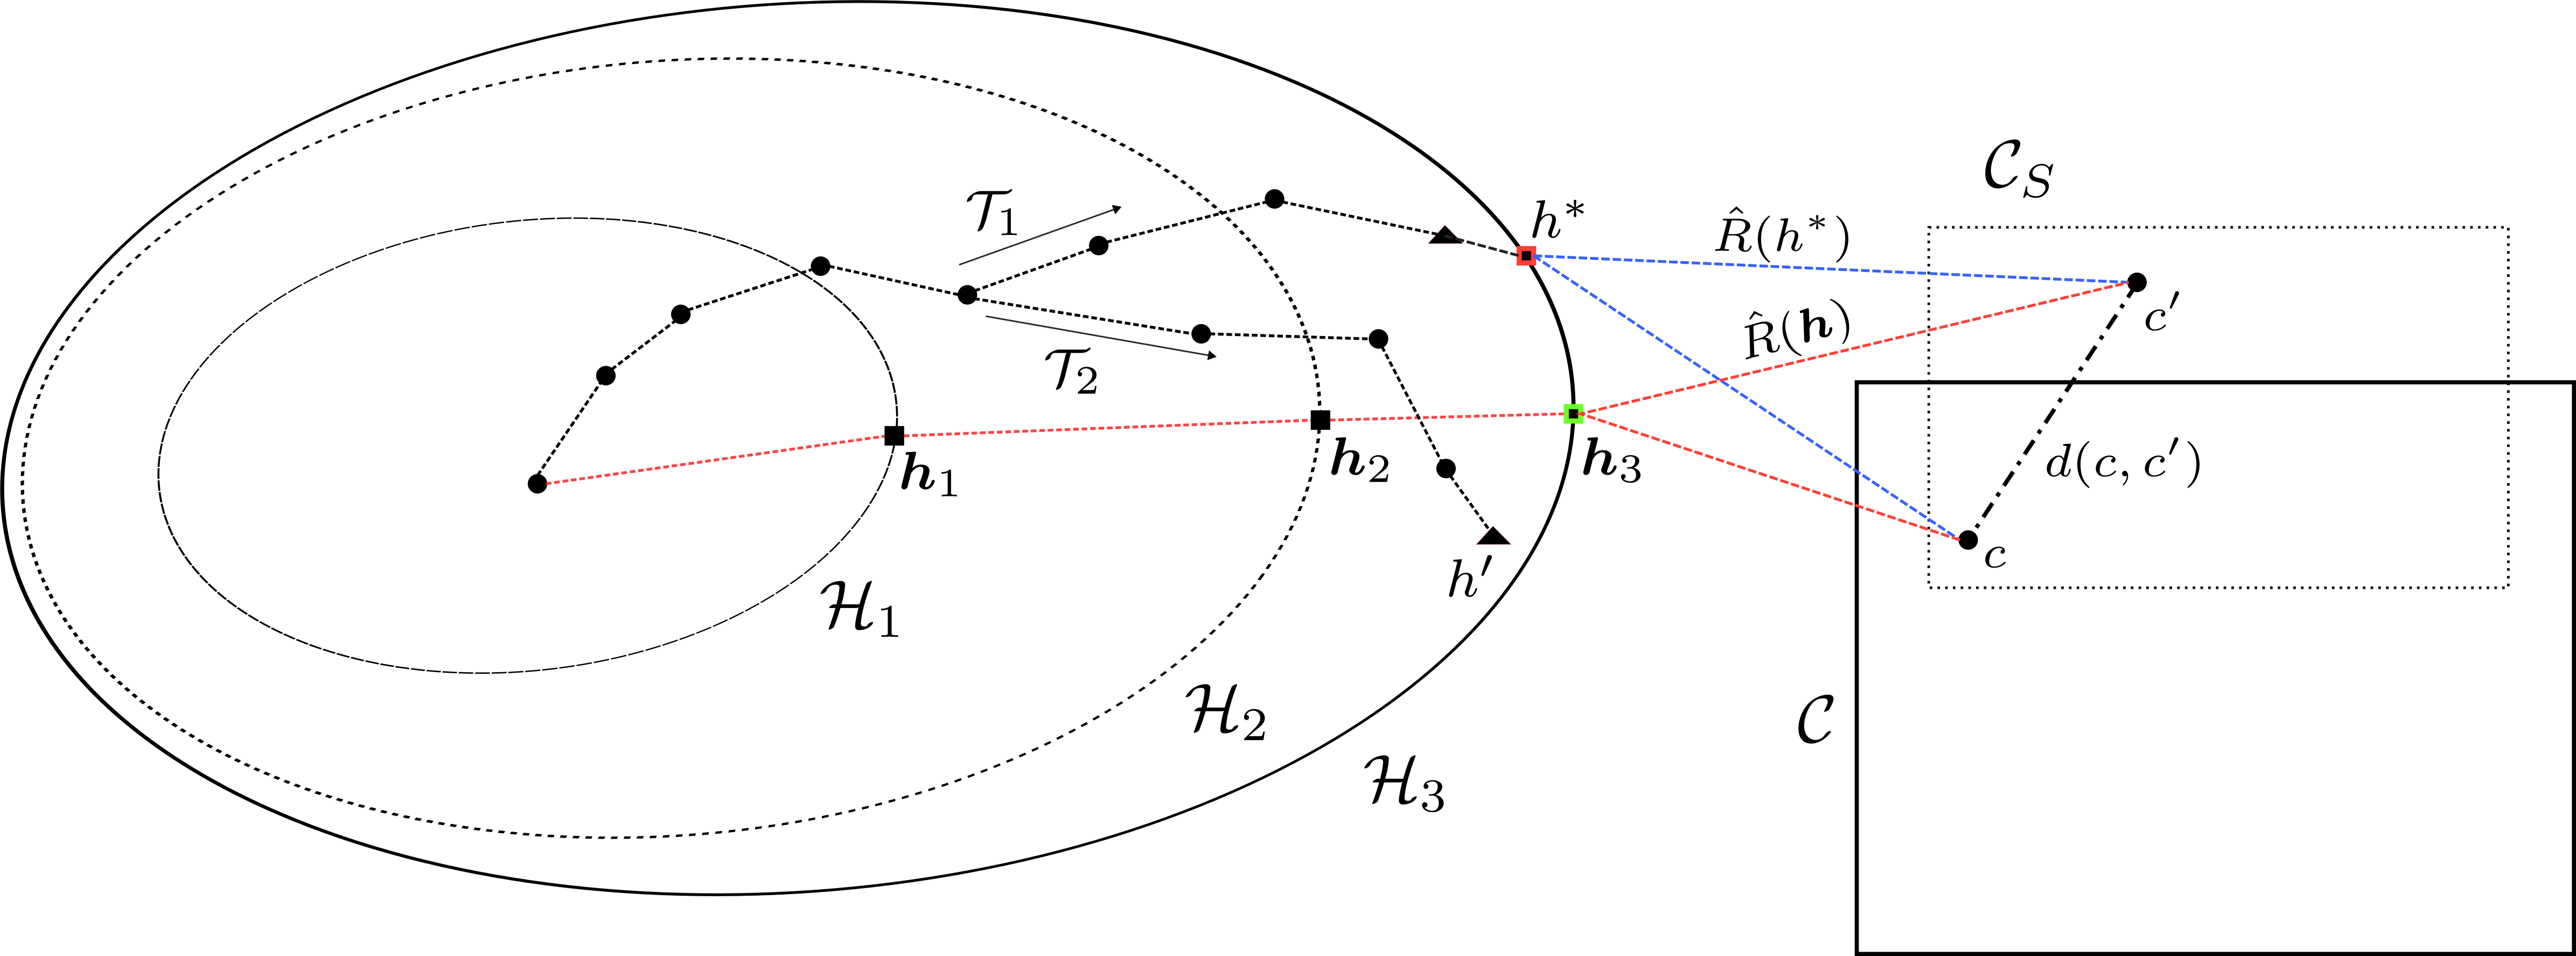
\includegraphics[width=0.9\textwidth]{g10.png}
  \caption{\textbf{Illustrative dynamic of the learning problem.} For an incremental hypothesis space sequence $\mathcal{H}_{1},\mathcal{H}_{2},\mathcal{H}_{3}$, we aim to obtain the procedure $\mathcal{T}$ that would either reach the \textit{generalization solution} $\bm{h}$, or the \textit{empirical solution} $h^{*}$ for a particular hypothesis class, with respect to the concept $c$ and its observed concept $c'$. Model selection hence dictates how an algorithm or procedure than choose the best possible hypothesis to approximate the generalization solution from the empirical solution set. Do notice that here we explicitly state that the data would create a \textbf{proxy concept} that overlaps with the concept class and of some arbitrary `distance' from the true concept by $d(c,c')$. In case the two classes overlap, there still exists the arbitrary distance. Also, we can also observe the intuitive notion of increasing hypothesis class - while it indeed can help in getting closer to the concept class, the somewhat intrinsic property of current learning theory being the relative random procedure class make it probabilistically unstable.}
  \label{fig:statlearnclassical}
\end{figure}

For fixed $\mathcal{H}$, for fixed and sufficiently large $\mathcal{S}$, and no observation (data) errors, the empirical risk is the generalization risk. These two measures between $h$ and $c$ constitute the learning problem, which can also be separated into both cases - either empirical learning or generalization learning, one to minimize $\hat{R}(h)$, and one to minimize $R(h)$. 

\begin{definition}[Empirical learning problem]
    We present the formal form of the empirical learning. Suppose we have a \textbf{target}, $c\in\mathcal{C}$, where $\mathcal{C}$ is an arbitrary concept class that captures targets of the same type. Suppose we are provided a set of observations $\mathcal{S}$. The problem is to use certain algorithm $\mathcal{A}$ using $\mathcal{S}$, to obtain a hypothesis $h^{*}$ for a fixed $\mathcal{H}$ such that: 
    \begin{equation}\label{eq:lp1}
        R(h^{*}) = \min_{h\in\mathcal{H}} \hat{R}(h) = \min_{h\in\mathcal{H}} \underset{x\sim\mathcal{D}, x\in \mathcal{S}}{\mathbb{E}}\:\ell\{h(x),c(x)\}
    \end{equation} 
\end{definition}

The generalization best $\bm{h}$ is also called in literature as the \textit{Bayes model}, such that it reduces the Bayes risk that is the infimum of the generalization risk, $R^{*}=\inf_{h\in \mathcal{H}}R(h)$. The hypothesis $h^{*}$ is often called the \textit{empirical best}, for it being the minimal, finite hypothesis of the lowest loss evaluation on the entire observation space $\mathcal{S}$. There exists no certified assumption regarding whether $h^{*}$ aligns with the minimal generalization error.

\begin{definition}[Generalization learning problem]
    We present the formal form of the generalization learning problem. Suppose we have a \textbf{target}, $c\in\mathcal{C}$, where $\mathcal{C}$ is an arbitrary concept class that captures targets of the same type. Suppose we are provided a set of observations $\mathcal{S}$. Supposed we have an algorithm $\mathcal{A}$ that for fixed hypothesis space $\mathcal{H}$, \eqref{eq:lp1} holds true. The problem is to use certain algorithm $\mathcal{A}'$ such that, under limited availability, to obtain $\bm{h}$, satisfies: \begin{equation}
        R(\bm{h}) = \min_{h\in \mathcal{H}} R(\bm{h}) \leq \{\epsilon\}, \quad \epsilon > 0 
    \end{equation}
    For a set of risk bounds $\epsilon$. If the setting is deterministic, then there exists $\epsilon=0$. 
\end{definition}

Then, we can partially say that generalization problem is an advancement from empirical solution. As such, empirical solution imposes the observed concept, and not the concept itself. This is reflected in modern machine learning landscape, by modelling the concept as distributions, and then using notions such as KL-divergence to measure such relative disparity. 

These two stages of learning procedure comes of as the intrinsic design of machine learning setting. As opposed to interpolation, where empirical learning problem would have to be put into first priority to achieve the best possible point-through model, machine learning leans on approximation more and a separated criterion that is only visible in the learning setting - the fact that we are using $c'$ to extract $c$. This disparity is exactly the \textbf{generalization problem}, of which is then also the goal of machine learning, to approximate the general solution using the observed solution. One then can ask what is the difference between the two notions, and when we can guarantee that both will `converge' to the same point. The process of \textbf{model selection} is then the procedure that will optimize $h\in \mathcal{H}$ to a given target fixture, such as the empirical best. 

One of the major assumption or observation from the point of the hypothesis class, is that the hypothesis cannot know the generalization error. Thereby, the more efficient and often used procedure/algorithm in training, is then the \textit{empirical risk minimization} (ERM) method, minimizing only the empirical risk to the empirical best; then, certain measures to `generalize' this heuristically is apprehended on the hypothesis. The process of model selection is also the place that we get the concept of \textbf{bias-variance tradeoff}. 
\subsubsection{Uniform convergence}

Suppose that for a concept class $\mathcal{H}$, we can then partition it to $\mathcal{H}=\bigcup_{k\in \mathbb{N}} \mathcal{H}_{k}$ for finite $k$ hypotheses. Assume that they satisfy the uniform convergence (\cite{JMLR:v11:shalev-shwartz10a}): 

\begin{equation}
    \sup_{\mathcal{D}} \underset{S\sim\mathcal{D}^{m}}{\mathbb{E}} \left[ \sup_{h\in\mathcal{H}} [R(h) - R_{S}(h)] \right] \overset{m\to\infty}{\longrightarrow} 0
\end{equation}

This uniform convergence holds for a learning problem, if the empirical risks of hypotheses in the hypothesis class converges to their population risk uniformly, with a distribution-independent rate. The result of this is that a problem then can be considered learnable with the ERM rule, for any given characterization. We state the following definition.

\begin{definition}
    A learning problem is learnable if there exist a learning rule $\mathcal{A}$ and a monotonically decreasing sequence $\epsilon_{cons}(m)$ such that $\epsilon_{cons}(m)\overset{m\to\infty}{\longrightarrow} 0$ and \begin{equation}
        \forall \mathcal{D} , \quad \underset{S\sim\mathcal{D}^{m}}{\mathbb{E}} \left[F(\mathcal{A}(S))-F^{*}\right] \leq \epsilon_{cons}(m) , \quad F^{*} = \inf_{h\in\mathcal{H}} R(h)
    \end{equation}
    A learning rule $\mathcal{A}$ for which this hold is denoted as a universally consistent learning rule. 
\end{definition}

There are certainly a fundamental class of rule or algorithm $\mathcal{A}$ to resolve this particular uniform convergence of classes. One of the major assumption or observation from the point of the hypothesis class, is that the hypothesis cannot know the generalization error. Thereby, one strategy is the \textit{empirical risk minimization} (ERM) method, minimizing only the empirical risk to the empirical best; then, certain measures to `generalize' this heuristically is apprehended on the hypothesis. 

\begin{definition}
    A rule $\mathcal{A}$ is an ERM (Empirical Risk Minimizer), denoted $\mathcal{A}_{ERM}$ if it minimizes the empirical risk $\hat{R}(h)=(1/m)\sum_{c\in\mathcal{C}}\ell(h,c)$, over the observational space $S$, 
    \begin{equation}
        \hat{R}_{S}(\mathcal{A}_{ERM}(S)) = \hat{R}_{S} (h_{S}) = \inf_{h\in\mathcal{H}} \hat{R}_{S}(h) 
    \end{equation}
    Hence, the ERM tries to obtain $\mathrm{ERM}(h') = \argmin_{h\in \mathcal{H}} \hat{R}(h)$. 
\end{definition}

The problem of overfitting still somewhat resides in the setting of the method. Hence, usually, we have an implicit term in addition, called the \textit{regularizer}, of which is as followed. 

\begin{definition}
    A rule $\mathcal{A}$ is an SRM (Structural Risk Minimizer), denoted $\mathcal{A}_{ERM}$ if it minimizes the empirical risk $\hat{R}(h)=(1/m)\sum_{c\in\mathcal{C}}\ell(h,c)$, over the observational space $S$, 
    \begin{equation}
        \hat{R}_{S}(\mathcal{A}_{SRM}(S)) = \hat{R}_{S} (h_{S}) + \lambda r(h)= \inf_{h\in\mathcal{H}} \hat{R}_{S}(h) + \lambda r(h)
    \end{equation}
    of the regularizing term $r(\cdot)$. Hence, the SRM tries to obtain $\mathrm{ERM}(h') = \argmin_{h\in \mathcal{H}} \hat{R}(h)$, while taking into consideration a forcing term $r$, usually defined on the model complexity. 
\end{definition}

In this research, we would like to presume the ERM method in question as the famous \textit{gradient descent}. We refer to \cite{achlioptas_stochastic_nodate,ruder_overview_2017} for general view of the algorithm, and \cite{zhang_gradient_2019} for a source on particularly gradient descent algorithm on deep learning models. 

%\begin{equation}
%    \forall k \in \mathbb{N}, \quad \underset{S\sim \mathcal{D}^{m}}{\mathbb{P}} \left%(\sup_{h\in \mathcal{H}_{k}} R(h) - \hat{R}_{S}(h)\leq \epsilon_{k}(m,\delta)\right) %\geq 1- \delta
%\end{equation}
%for functions $\epsilon_{k}$ satisfies that for all $k$ and $\delta\in (0,1)$, $\lim_%{m\to\infty}\epsilon_{k}=0$. One of the major assumption or observation from the point %of the hypothesis class, is that the hypothesis cannot know the generalization error. %Thereby, the more efficient and often used procedure/algorithm in training, is then the %\textit{empirical risk minimization} (ERM) method, minimizing only the empirical risk to %the empirical best; then, certain measures to `generalize' this heuristically is %apprehended on the hypothesis:
%\begin{equation}
%        \mathsf{ERM}(h') = \argmin_{h\in \mathcal{H}} \hat{R}(h)
%    \end{equation}
%Another way is to use the \textit{structural risk minimization} (SRM) method, which add %a regularizer $r(\cdot)$ after the empirical error,
%\begin{equation}
%        \mathsf{SRM}(h') = \argmin_{h\in \mathcal{H}} \hat{R}(h) + \lambda r(h)
%    \end{equation}
%The regularizer term $r(\cdot)$ takes of its argument the model, and calculate based of %certain measure of its complexity. Thereby, the goal is to penalize structures with high %complexity and favour simpler designs, in principle.
%
%In this research, we would like to presume the ERM method in question as the famous %\textit{gradient descent}. We refer to \cite{achlioptas_stochastic_nodate,%ruder_overview_2017} for general view of the algorithm, and \cite{zhang_gradient_2019} %for a source on particularly gradient descent algorithm on deep learning models. %Nominally, for the $n$th output sequence $w_{n}$, it updates the model to a given path %of optimization for $w_{n+1}$ such that 
%\begin{equation}
%    w_{n+1} = w_{n} - \alpha_{n}\nabla_{w_{n}}(\mathcal{L}(h(x),y))
%\end{equation}
%for $\alpha_{n}\geq 0$ the step size of the iteration, and with a (potentially) convex %function $\mathcal{L}(h(x),y)$ of the hypothesis class $\mathcal{H}$. 
%

\section{Double descent, the problem}

One of the major assumption or observation from the point of the hypothesis class, is that the hypothesis cannot know the generalization error. Thereby, the more efficient and often used procedure/algorithm in training, is then the \textit{empirical risk minimization} (ERM) method, minimizing only the empirical risk to the empirical best; then, certain measures to `generalize' this heuristically is apprehended on the hypothesis. The process of model selection is also the place that we get the concept of \textbf{bias-variance tradeoff}. And it is also where we will have our dilemma of double descent, as will be discovered later. 

\subsection{Bias-variance tradeoff}

Bias-variance tradeoff comes off from a statistical approach, predate machine learning by itself. The theory that bias and variance often come in to conjunction is \textbf{Estimation theory}, of which there exists an estimator $\hat{\theta}$ that use a set of observations, to estimate the concept, or the underlying mechanics of certain system that outputted the observation set, by the \textbf{probabilistic perspective} - that is, it is governed by appearance by an independently and identically distributed process of parameterized probability $\theta\in \Theta$. Here, parameterized means being expressed by a set, often finite, of parameters, by \cite{LehmannCasella_theory_1998,liam_statistics_2005}. 
\subsubsection{Statistical origin}
As we have said, the notion comes from statistical analysis. In such, there are two important functions associated with any estimator $\hat{\theta}$ that are useful as a thumbnail sketch on how well the estimator is doing (\cite{liam_statistics_2005}), the \textit{bias} and the \textit{variance}. Classically, estimation theory is concerned of the problem of data sample estimation on continuous real line $\mathbb{R}$. As such, the ultimate goal of classical estimation theory is the minimization of the estimator mean square error (MSE), that is given as 
\begin{equation}
  \mathsf{MSE}(\hat{\theta}) \triangleq \mathbb{E}_{y} \lvert \lvert \hat{\theta} - \theta \rvert \rvert^{2} = \mathbb{E}_{y} \lvert\lvert z(y) - \theta \rvert \rvert^{2}
\end{equation}
where $y$ is the observation set by notation, and $\hat{\theta}=z(y)$ is the estimator of interest. Then, the bias and variance is defined to be
\begin{equation}
  \mathsf{Bs}(\hat{\theta}) = \lvert\lvert \mathbb{E}_{y} \{\hat{\theta} - \theta\}\rvert\rvert, \quad \mathsf{Var}(\hat{\theta}) = \mathbb{E}_{y} \lvert\lvert \hat{\theta} - \mathbb{E}_{y} \{\hat{\theta}\}\vert\rvert^{2}
\end{equation}
This prompted a tradeoff, in which for the mean squared error the \textbf{minimum mean squared error} (MMSE) estimator would consider the bias and variance for every value of the parameterized descriptor $\theta$. The best strategy potentially can be employed is then to reduce the variance of the model. This is rationalized as because for estimation theory in general, the bias term is unrealizable because it depends on the measure of the true concept. Based on the probabilistic interpretation, the true concept, or its true parameters governing the probabilistic sampling process cannot be learned, and hence the term bias can be at best approximated, with varied degree of accuracy. The limitation (\cite{piera_sample_2005,MkayPretenceSignalStatistics1993}) suggests to focus uniquely on unbiased estimators holding that $\mathsf{Bs}(\hat{\theta})=0$. Thus, the estimator mean square measure is equal to its variance, and the resulting estimator is then referred to as the minimum variance unbiased (MVU) estimator by \cite{MkayPretenceSignalStatistics1993}. 

In modern literature, the analysis of machine learning model and the introduction of such bias-variance concept for model selection criterion first came from \cite{6797087}. Of a later date, there are many interpretations, and similar notions of such tradeoff comes from both statistical learning theory and his original paper, which is used extensively among modern machine learning practicians. 
\subsubsection{Precursor (Geman et al., 1992)}

The original definition of bias-variance tradeoff by \cite{6797087} is first constructed using the means-square error, which is regarded as a normal measure in the real encoding space. Their approach is to justify bias-variance via decomposition of the loss function $\ell$, for such to find an alternative reasonable form of such loss landscape. Suppose of a regression problem to construct a hypothesis function $f(x)$ from $(x_{1},y_{1},\dots,x_{N},y_{N})$ for the purpose of generalization - that is, predicting unseen variational values for different pair $(x_{j}, \mathord{?})$ such that $\mathord{?}=y_{j}+\epsilon$ for a conceivable implicit error. To be explicit about the relation of this problem, or $f$ on the given data $\mathcal{D}=\{(x_i, y_i)\mid i \leq N\}$, denote $f(x;\mathcal{D})$ instead of $f$, the natural mean-square measure as a predictor is: 
\begin{equation}
    \mathcal{M}(f,y) = \mathbb{E} \left[((y-f(x;\mathcal{D})))^{2}\mid x, \mathcal{D}\right] 
\end{equation} for $\mathbb{E}[\cdot]$ the expectation wrt to a distribution $P$. Decomposing the right-hand side, we have: 
\begin{equation}
    \mathcal{M}(f,y) = \mathbb{E} \left[((y-f(x;\mathcal{D})))^{2}\mid x, \mathcal{D}\right] = \mathbb{E}\left[(y-\mathbb{E}[y\mid x])^{2}\mid x,\mathcal{D}\right] + (f(x;\mathcal{D})-\mathbb{E}[y\mid x])^{2}
\end{equation}
Here, $\mathbb{E}\left[(y-\mathbb{E}[y\mid x])^{2}\mid x,\mathcal{D}\right]$ does not depend on $\mathcal{D}$, but simply the statistical variance of $y$ given $x$. The term $(f(x;\mathcal{D})-\mathbb{E}[y\mid x])^{2}$ is considered a natural measure of effectiveness on $\mathbb{R}^{n}$ as a singular predictor of $y$. Now, for $\mathbb{E}_{\mathcal{D}}\left[(f(x;\mathcal{D})-\mathbb{E}[y\mid x])^{2}\right]$ which depends on the training set $\mathcal{D}$ in its computation, is decomposed into the form of \textit{bias-variance decomposition} terms, by derivation: 
\begin{equation}
    \begin{split}
        \mathbb{E}_{\mathcal{D}} \left[(f(x;\mathcal{D})-\mathbb{E}[y\mid x])^{2}\right] & = \underbrace{\left\{ \mathbb{E}_{\mathcal{D}}[f(x;\mathcal{D})] - \mathbb{E}[y\mid x] \right\}^{2}}_{\text{bias term}} + \underbrace{\mathbb{E}_{\mathcal{D}} \left\{(f(x;\mathcal{D})- \mathbb{E}_{\mathcal{D}}[f(x;\mathcal{D})])^{2}\right\}}_{\text{variance term}}
    \end{split}
\end{equation}

We summarize this in the following statement. 

\begin{theorem}[Bias-variance decomposition]
    Suppose the model $f(x;\mathcal{D})$ for the data $\mathcal{D}=(x_i, y_i)$ and its parameter $x$ is defined. For $y_{i}$ of the target concept's responses $y$, and consider a regression problem with the loss measure $\mathcal{M}(f,y)$ of mean squared risk, the following statement is true: \begin{equation}
        \mathbb{E}\big[\mathcal{M}(f,y)\big] = \mathcal{B}(f,y) + \mathcal{V}(f,y) + \mathbb{E}\Big[\mathbb{E} \left[((y-f(x;\mathcal{D})))^{2}\mid x, \mathcal{D}\right]\Big]
    \end{equation}
    for $\mathbb{E}[\:\cdot\mid x, \mathcal{D}]$ any expression with dependencies on $x$ and $\mathcal{D}$. The bias and variance term is subsequently expressed by 
    \begin{align}
        \mathcal{B}(f,y) = \underbrace{\left\{ \mathbb{E}_{\mathcal{D}}[f(x;\mathcal{D})] - \mathbb{E}[y\mid x] \right\}^{2}}_{\text{bias }}, \quad \mathcal{V}(f,y) =\underbrace{\mathbb{E}_{\mathcal{D}} \left\{(f(x;\mathcal{D})- \mathbb{E}_{\mathcal{D}}[f(x;\mathcal{D})])^{2}\right\}}_{\text{variance}}
    \end{align}
\end{theorem}

The above decomposition principle is often expressed into a form where there exists the intrinsic noise \cite{brown2024biasvariance}: 
\begin{equation}
    \begin{split}
        \mathbb{E}_D \left[ \mathbb{E}_{xy} \left( y - \hat{f}(x) \right)^2 \right]
        &= 
         \mathbb{E}_x \left[ \left( y^* - \mathbb{E}_D[\hat{f}(x)] \right)^2 \right]
        + \mathbb{E}_x \left[ \mathbb{E}_D \left( \hat{f}(x) - \mathbb{E}_D[\hat{f}(x)] \right)^2 \right] \\
        &+ \mathbb{E}_{xy} \left[ \left( y - y^* \right)^2 \right]
    \end{split}
    \end{equation}
For simplicity of notation, we adopt the similar form in the standard case of \cite{adlam2020understandingdoubledescentrequires}: 
\begin{equation}
    \E \qa{\hat{y}(\bfx)-y(\bfx)}^2 = \pa{\E\hat{y}(\bfx) - \E y(\bfx)}^2 + \V\qa{\hat{y}(\bfx)} + \V\q{y(\bfx)}
\end{equation}
A main common theme of criticism toward bias-variance tradeoff is the fact that the decomposition is much more general, and intrinsic for the class of \textit{mean squared loss}. However, when considering the naturalness of an error measure and then its direct applicant, mean square error on real space of sufficient support and measure comes of as a very natural choice of an error measure, at least in consideration of the regression setting; for that, we then can also define classification as another top-layer above a regression's similar real continuous space, i.e. a decision layer. Furthermore, it can also be shown \cite{brown2024biasvariance,PfauBregmanDivergence} that it also holds for the class of Bregman divergence measure. 

What does the decomposition say about model selection principle in general? In general, bias-variance is typically presented of its decomposition only, and the asymptotic prediction of its behaviours. In fact, one of the reason that it became the rule-of-thumb for ML practitioner, as well as generally statistical learning (\cite{lafon_understanding_2024} provides a quite rigorous treatment of bias-variance tradeoff in the section on statistical learning theory) solidify the trade-off as a particular model selection principle. Generally, this tradeoff can be summarized as followed: 
\begin{theorem}[Bias-variance tradeoff]
    For the expected loss of any given hypothesis $h$, the bias $\mathcal{B}(f,y)$ and variance $\mathcal{V}(f,y)$ is inversely proportional, that is, $\mathcal{B}(f,y)\propto \lambda^{-1} \mathcal{V}(f,y)$ for some proportionality $\lambda$ that may or may not be constant. In the most general case possible, $\lambda = -1$ on the entire error range. 
\end{theorem}

The tradeoff is then of inverse proportionality. Indeed, statistically, we have such tradeoff on a statistical framework in a more concrete sense. For the bias to increase, variance will increase, of which the criterion is inverse - we would like to have more bias but lower variance, according to such theory. 

There are problems regarding such stance. The main problem is that generally, the bias-variance measure does not totally match the overall decomposition structure. Even with irreducible errors, there are factors which make it to incorporate other error factors in for the decomposition, of which is inexplainable. There are also works, for example, \cite{domingos_unifeid_2000}, of which decompose the error to 
\begin{equation*}
        \begin{split}
            \mathrm{Error} & = \lambda_{1} \mathrm{Bias}(f,y) + \lambda_{2}\mathrm{Var}(f,y)+ \lambda_{3}\epsilon(\mathcal{D})\\ 
            & = \lambda_{1}\underbrace{\left\{ \mathbb{E}_{\mathcal{D}}[f(x;\mathcal{D})] , \mathbb{E}[y\mid x] \right\}}_{\text{bias term}} +\lambda_{2} \underbrace{\mathbb{E}_{\mathcal{D}} \left\{(f(x;\mathcal{D}), \mathbb{E}_{\mathcal{D}}[f(x;\mathcal{D})])\right\}}_{\text{variance term}} +\underbrace{\lambda_{3}\epsilon}_{\text{irreducible error}}
        \end{split}
\end{equation*}
of which the bias-variance-irreducible error are `fit' into the total error by three coefficients $\lambda_{1},\lambda_{2},\lambda_{3}$ instead. This does not only scale up the B-V-IE triplet, but also leaves out the inexplainable gap between the scaling, and the actual normal measure. 

The bias-variance decomposition and tradeoff is not general. Indeed, works, by \cite{6797087,sharma_bias-variance_2014,domingos_unifeid_2000,adlam2020understandingdoubledescentrequires,yang_rethinking_2020} and more all attempted to reconstruct and reformulate bias-variance, and it did leave out a picture of uncertainty regarding the concept. 

\subsection{Double descent}

Nevertheless, of bias-variance and the analogous statistical learning theory concept, the target is the same. It is the dilemma of which is presented in \textbf{Occam's razor}, for choosing the sufficient model of good complexity, or bias, for tradeoff of its generalization ability, or variance. Then there must exist a sweet spot between the axis of bias and variance, since they are as exhibited above inversely proportional to each other. However, double descent seemingly broke the status quo, and insists on an interesting phenomenon - under the same setting, if we `crank' the complexity high enough, we will then reach a point then called the \textbf{interpolation threshold}, such that the trend reverse and the error rate, instead of being theorized to go up, goes down to a certain line of lower bound. 

The first identification of the double descent phenomena dated back to the paper of Belkin - \cite{belkin_reconciling_2019}, in which the title is literally "reconciling" modern machine learning practice and the bias-variance tradeoff. In modern machine learning practice, or state-of-the-art developments, models are now bigger than ever. If to notice, we will see that currently models are inherently large, for example, a normal large language model will have from 900 millions (900M) to a few billions, for example 10 billions (10B) parameters. That is not taking into account the overall dynamics and structure of the model, which dictates the operating range and efficiency of the model itself. These model, based on the neural network architecture are somewhat trained to exactly fit (or interpolate) the data, almost certainly so that it turn from a prediction setting to an estimation setting. By statistical learning theory, this would be considered overfitting, and yet, they often obtain very high accuracy on test data.

\begin{figure}[htb]
    \centering
    \begin{tabular}{cc}
    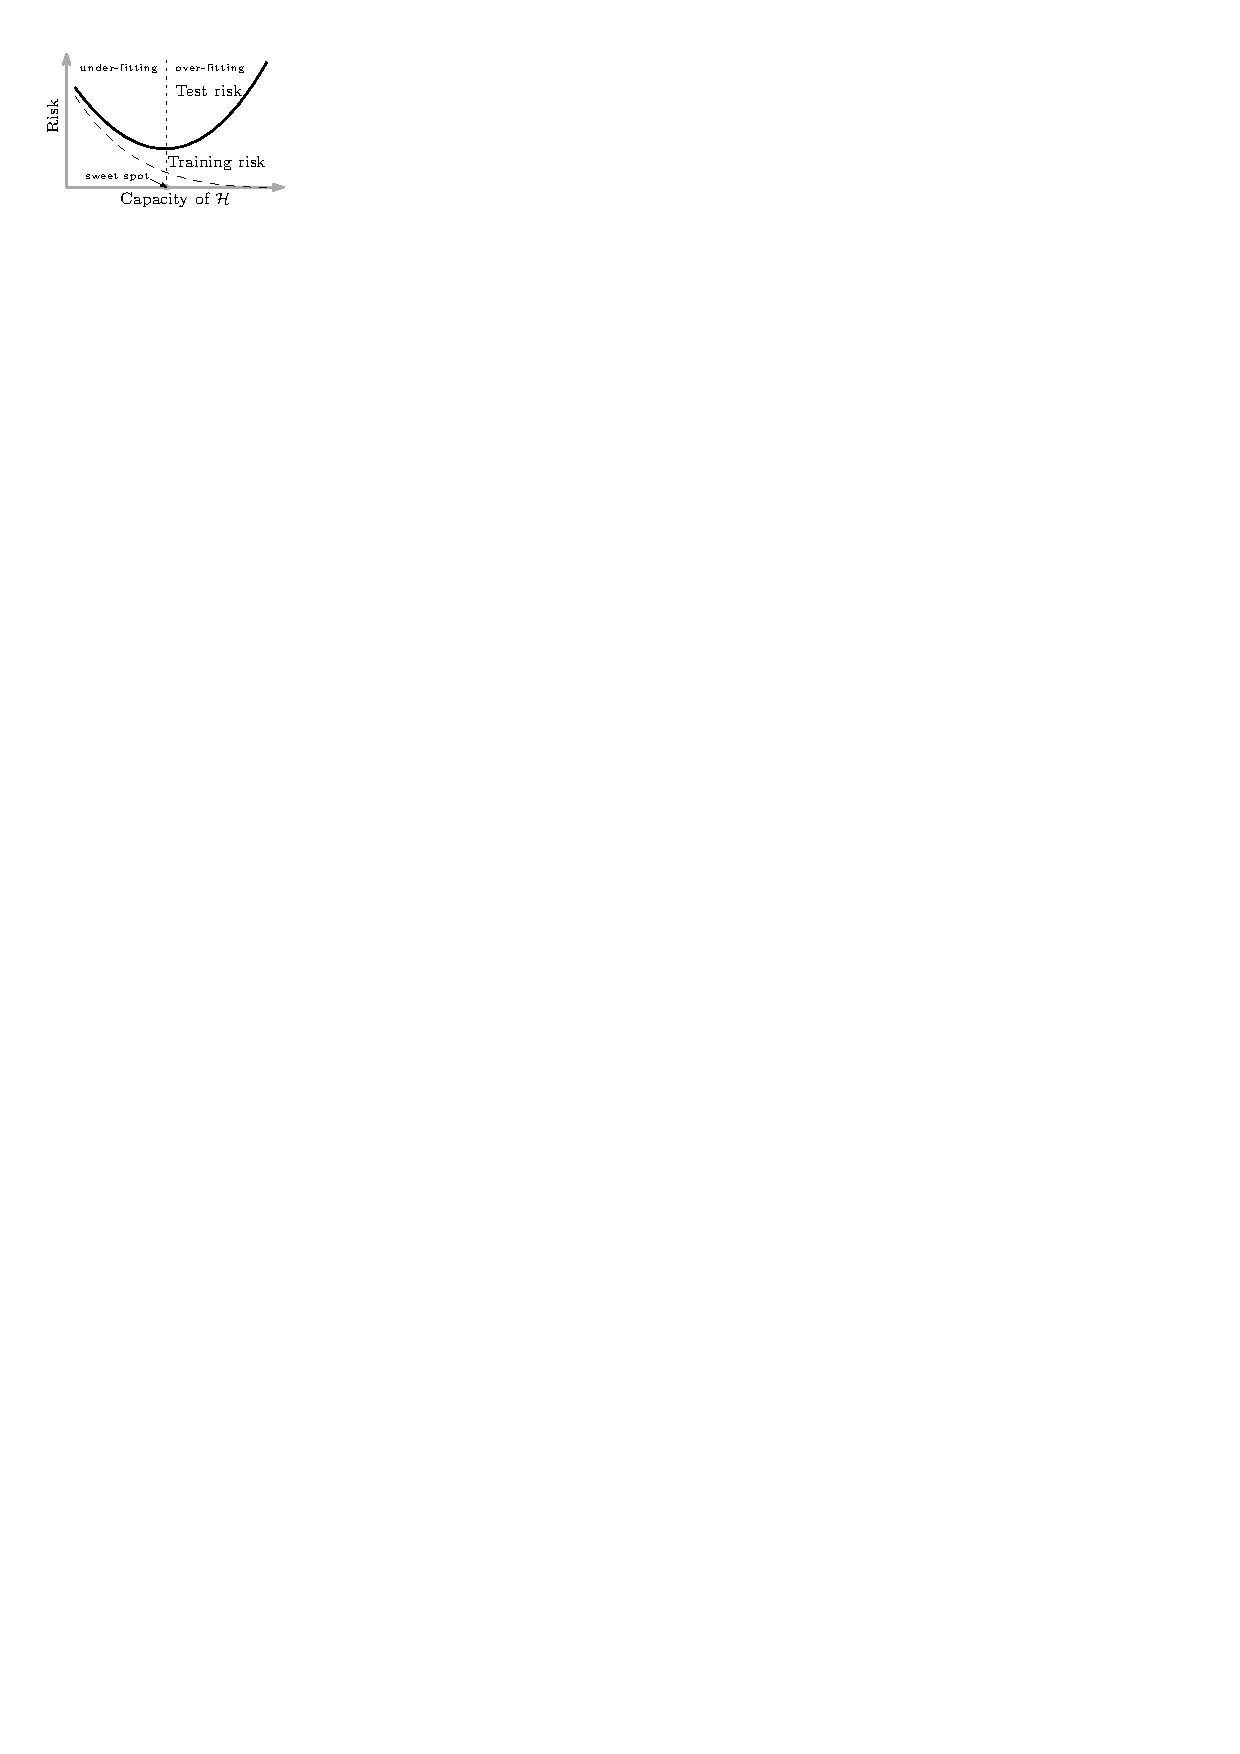
\includegraphics[height=0.15\textheight]{pdf/u-shaped.pdf} &
    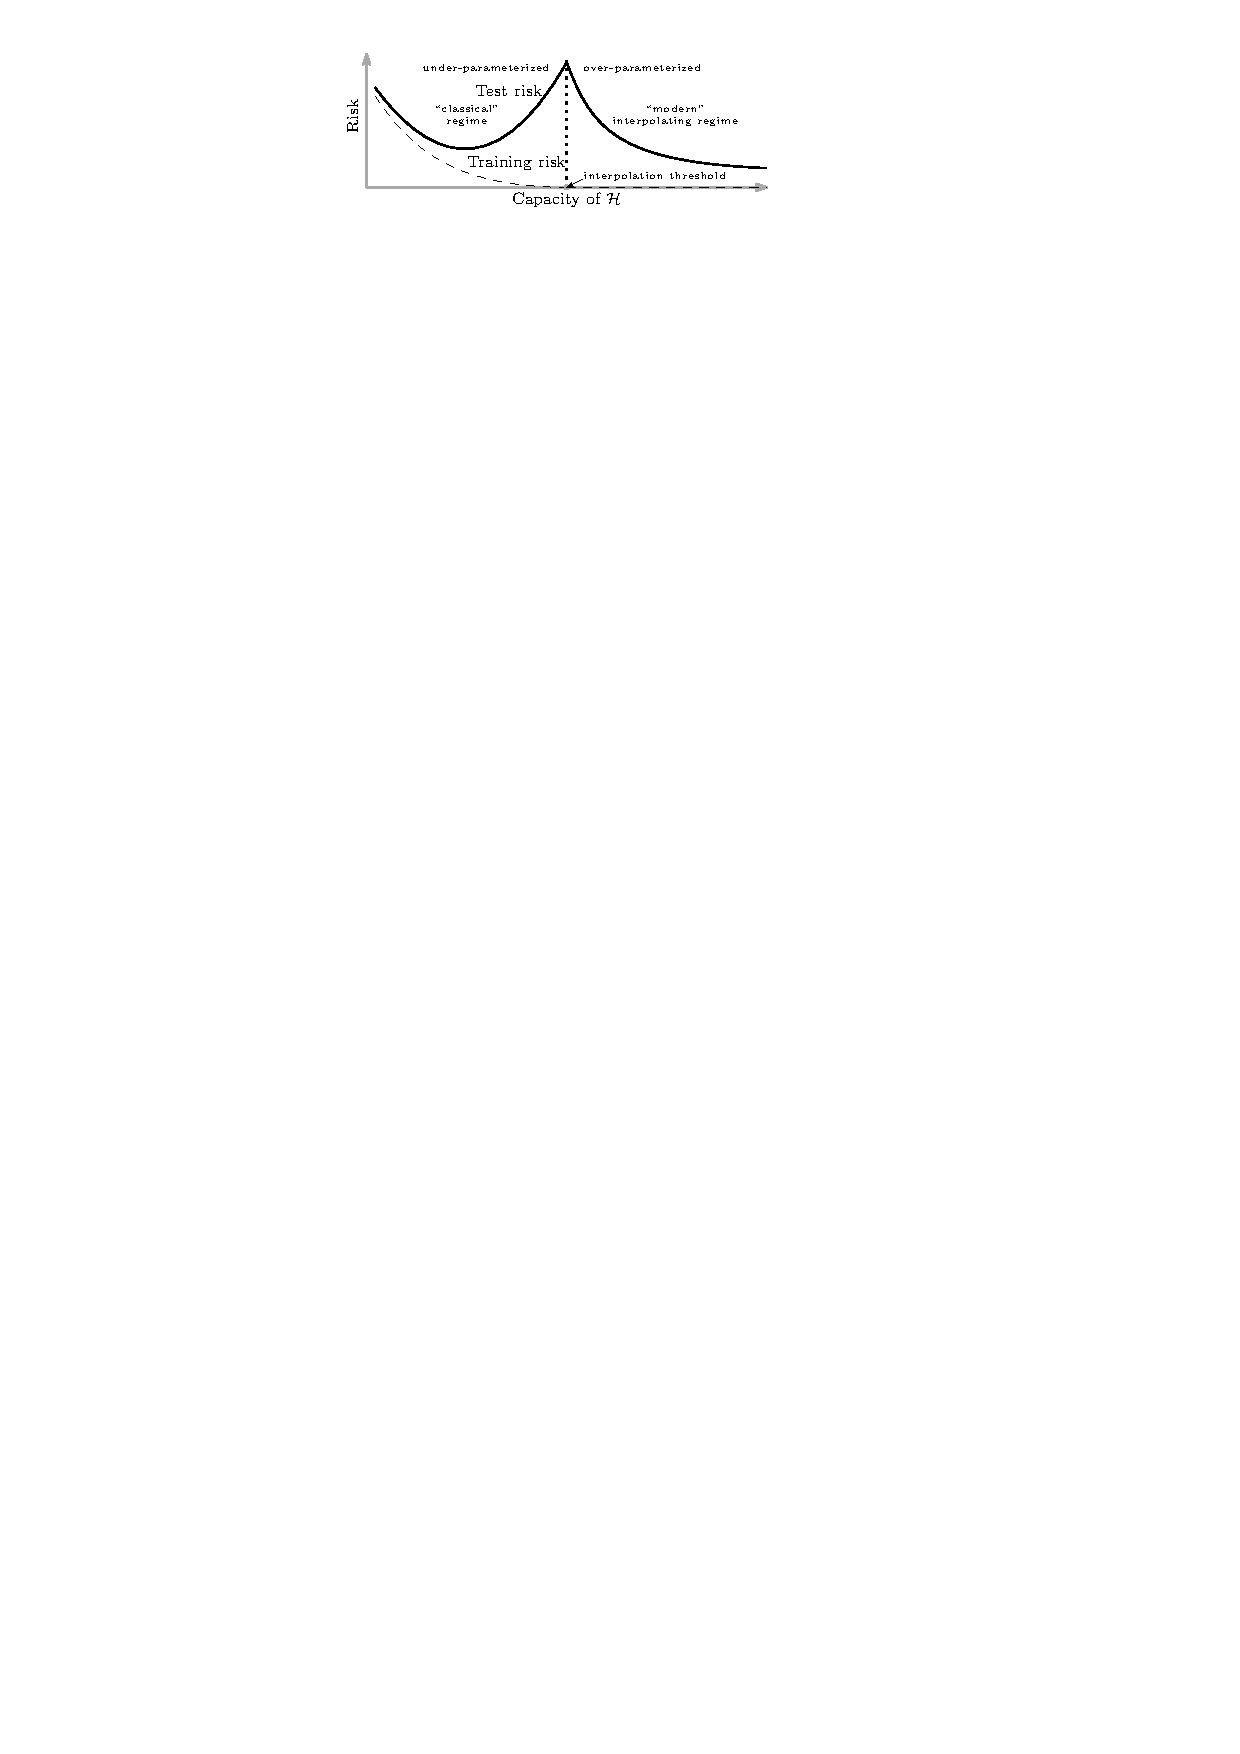
\includegraphics[height=0.15\textheight]{pdf/doubledescent.pdf} \\
    {\bf (a)} & {\bf (b)}
    \end{tabular}
    \caption{{\bf Curves for training risk (dashed line) and test risk (solid line).}
      ({\bf a}) The classical \emph{U-shaped risk curve} arising from the bias-variance trade-off.
      ({\bf b}) The \emph{double descent risk curve}, which incorporates the U-shaped risk curve (i.e., the ``classical'' regime) together with the observed behaviour from using high capacity function classes (i.e., the ``modern'' interpolating regime), separated by the interpolation threshold.
      The predictors to the right of the interpolation threshold have zero training risk. Reproduced from \cite{belkin_reconciling_2019}.}
    \label{fig:double-descent}
\end{figure}

The main finding that Belkin found is a pattern for how the apparent performance on unseen data depends on model capacity and the mechanism underlying the emergence of double descent. When function class capacity is below the "interpolation threshold", learned predictors exhibit the classical $U$-shaped curve from Figure~\ref{fig:double-descent}. The `modern' interpolating regime marks the opposite trend to the right, where the risk starts to decrease up to a lower bound, which then can be called the \textit{optimal descent bound}. 

\blockquote[\cite{belkin_reconciling_2019}]{The bottom of the $U$ is achieved at the sweet spot which balances the fit to the training data and the susceptibility to over-fitting:
to the left of the sweet spot, predictors are under-fit, and immediately to the right, predictors are over-fit.
When we increase the function class capacity high enough (e.g., by increasing the number of features or the size of the neural network architecture), the learned predictors achieve (near) perfect fits to the training data---i.e., interpolation.
Although the learned predictors obtained at the interpolation threshold typically have high risk, we show that increasing the function class capacity beyond this point leads to decreasing risk, typically going below the risk achieved at the sweet spot in the ``classical'' regime.}

Another prominent result to look at is \cite{nakkiran_deep_2019}, on the double descent of deep learning models. This is the first step toward identifying double descent to be perhaps, universal. 

\begin{figure}[htb]
    \centering
    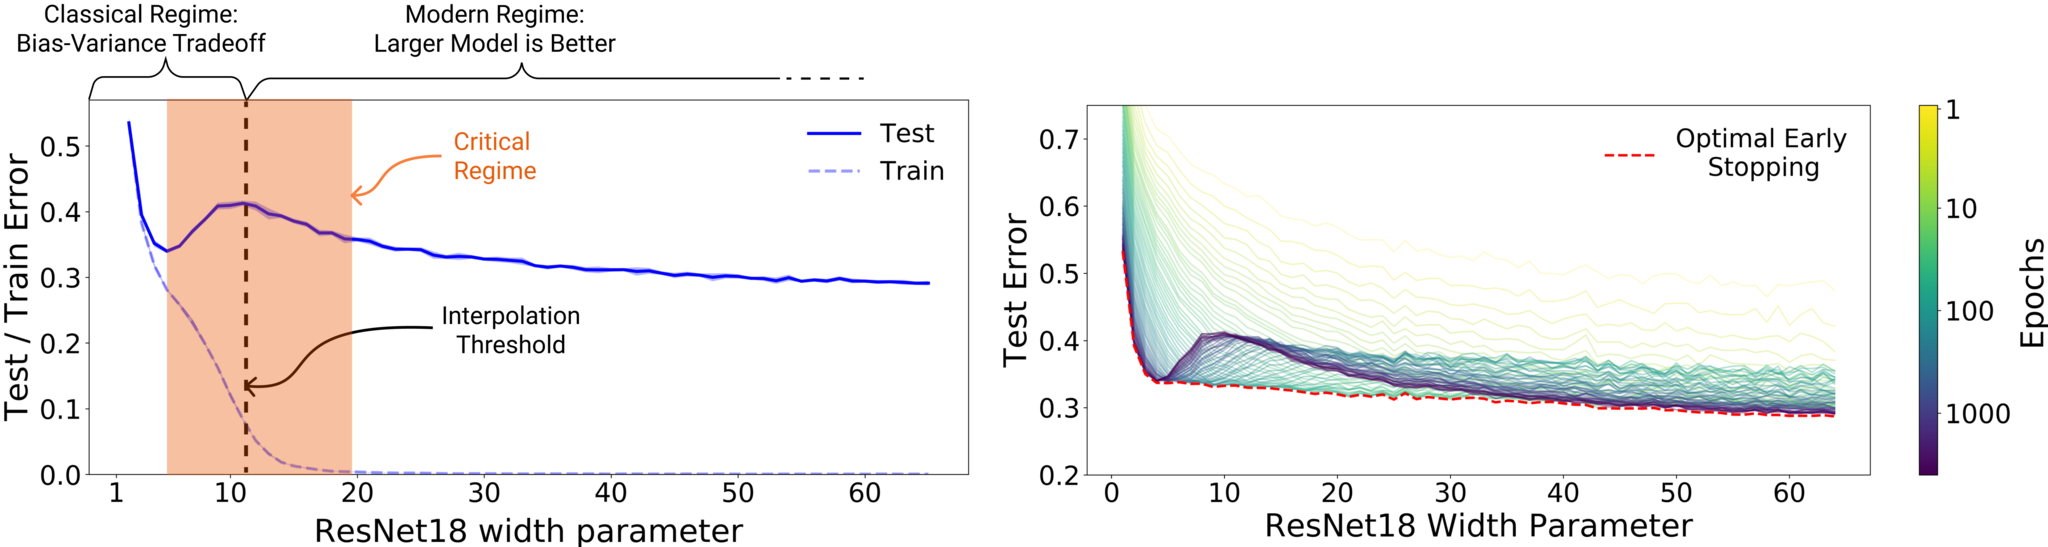
\includegraphics[width=1\textwidth]{media/errorvscomplexity.png}
    \caption{{\bf Left:} Train and test error as a function of model size,
    for ResNet18s of varying width 
    on CIFAR-10 with 15\% label noise.
    %In the under-parameterized regime, test error follows
    %the behavior predicted by classical statistical learning theory, but in the overparameterized regime (once training error is approximately zero),  the test error undergoes a ``second descent'' and decreases as model size increases. The shaded region represents the critically parameterized regime where the transition from under- to over-parameterization occurs. 
    {\bf Right:}
    Test error, shown for varying train epochs.
    %The dashed red line shows that with optimal early stopping double descent is not observed.
    % All models are ResNet18s of varying width,
    % trained on CIFAR10 with 15\% label noise
    All models trained using Adam for 4K epochs.
    %, and plotting means and standard-deviations from 5 trials with random network initialization.
    The largest model (width $64$) corresponds to standard ResNet18. Resued from \cite{nakkiran_deep_2019}.
    %    \ptodo{point out that interpolation point for second plot is plotted in the ocean plot}
    }
    \label{fig:errorvscomplexity}
\end{figure}

\begin{figure}[htb]
\centering
\begin{minipage}{.512\textwidth}
  \centering
  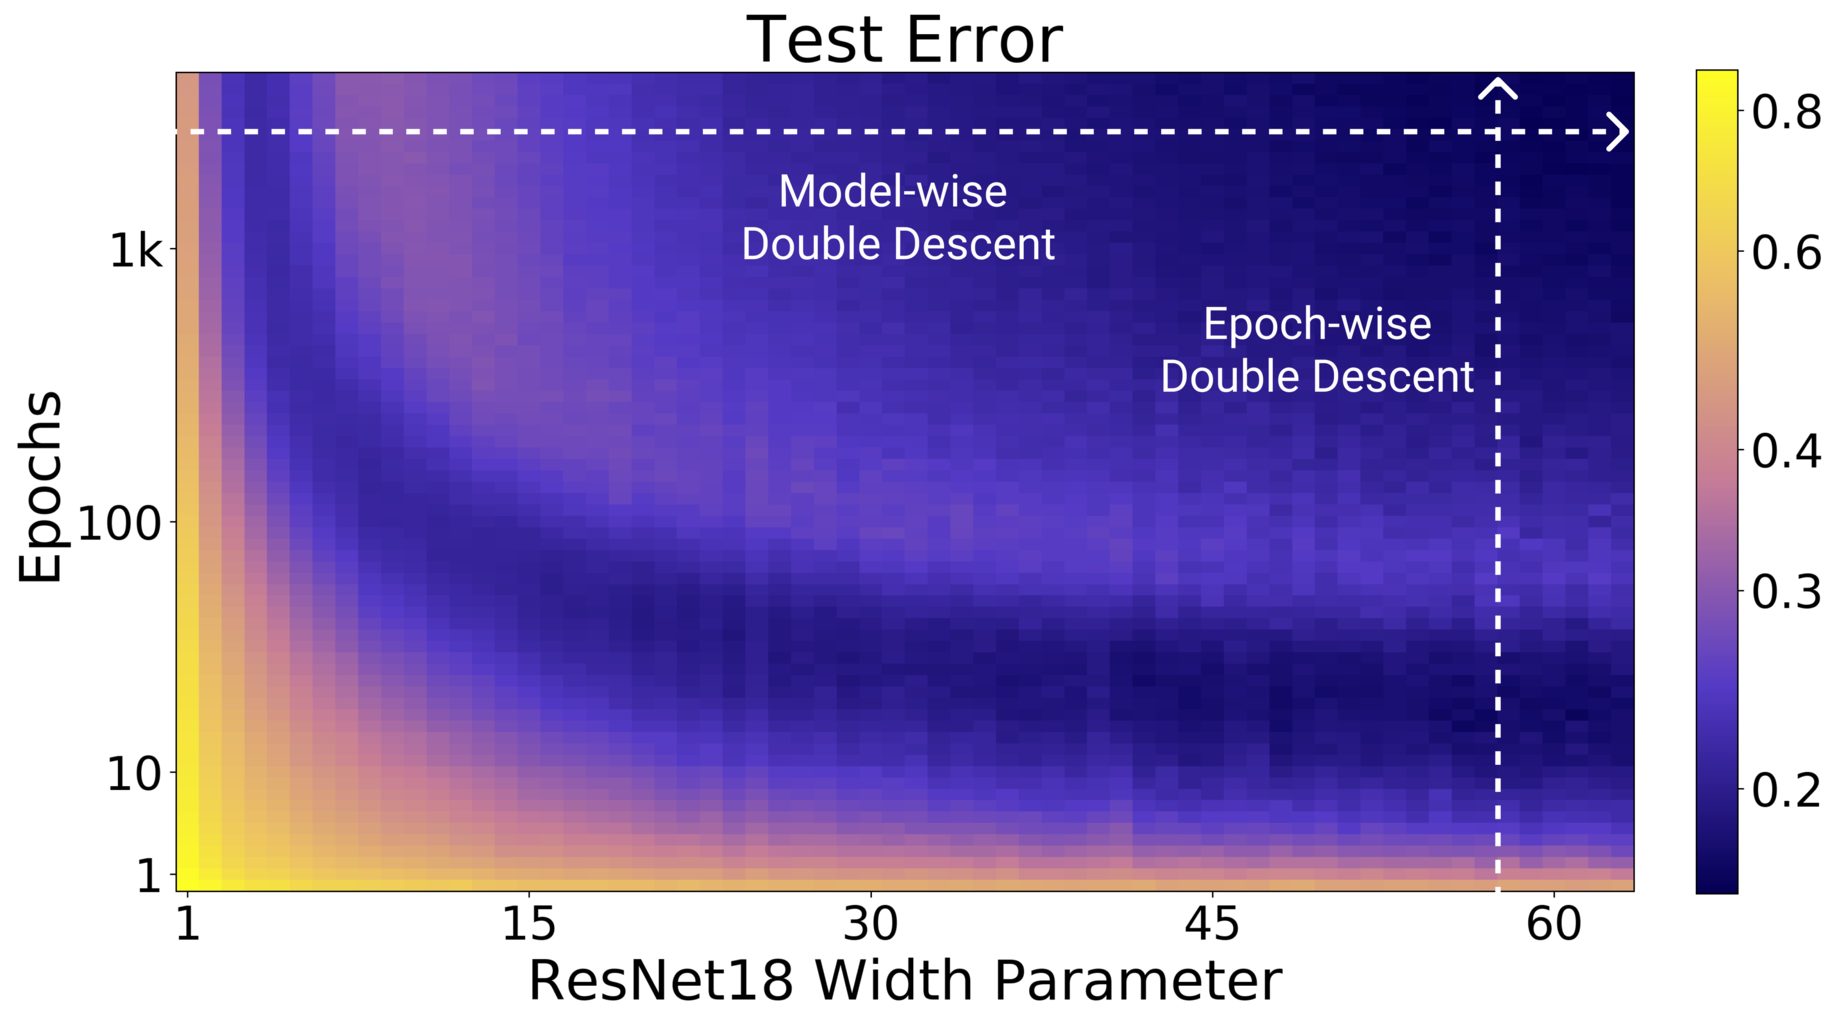
\includegraphics[width=1\textwidth]{media/Intro-ocean-test.png}
\end{minipage}%
\begin{minipage}{.488\textwidth}
  \centering
  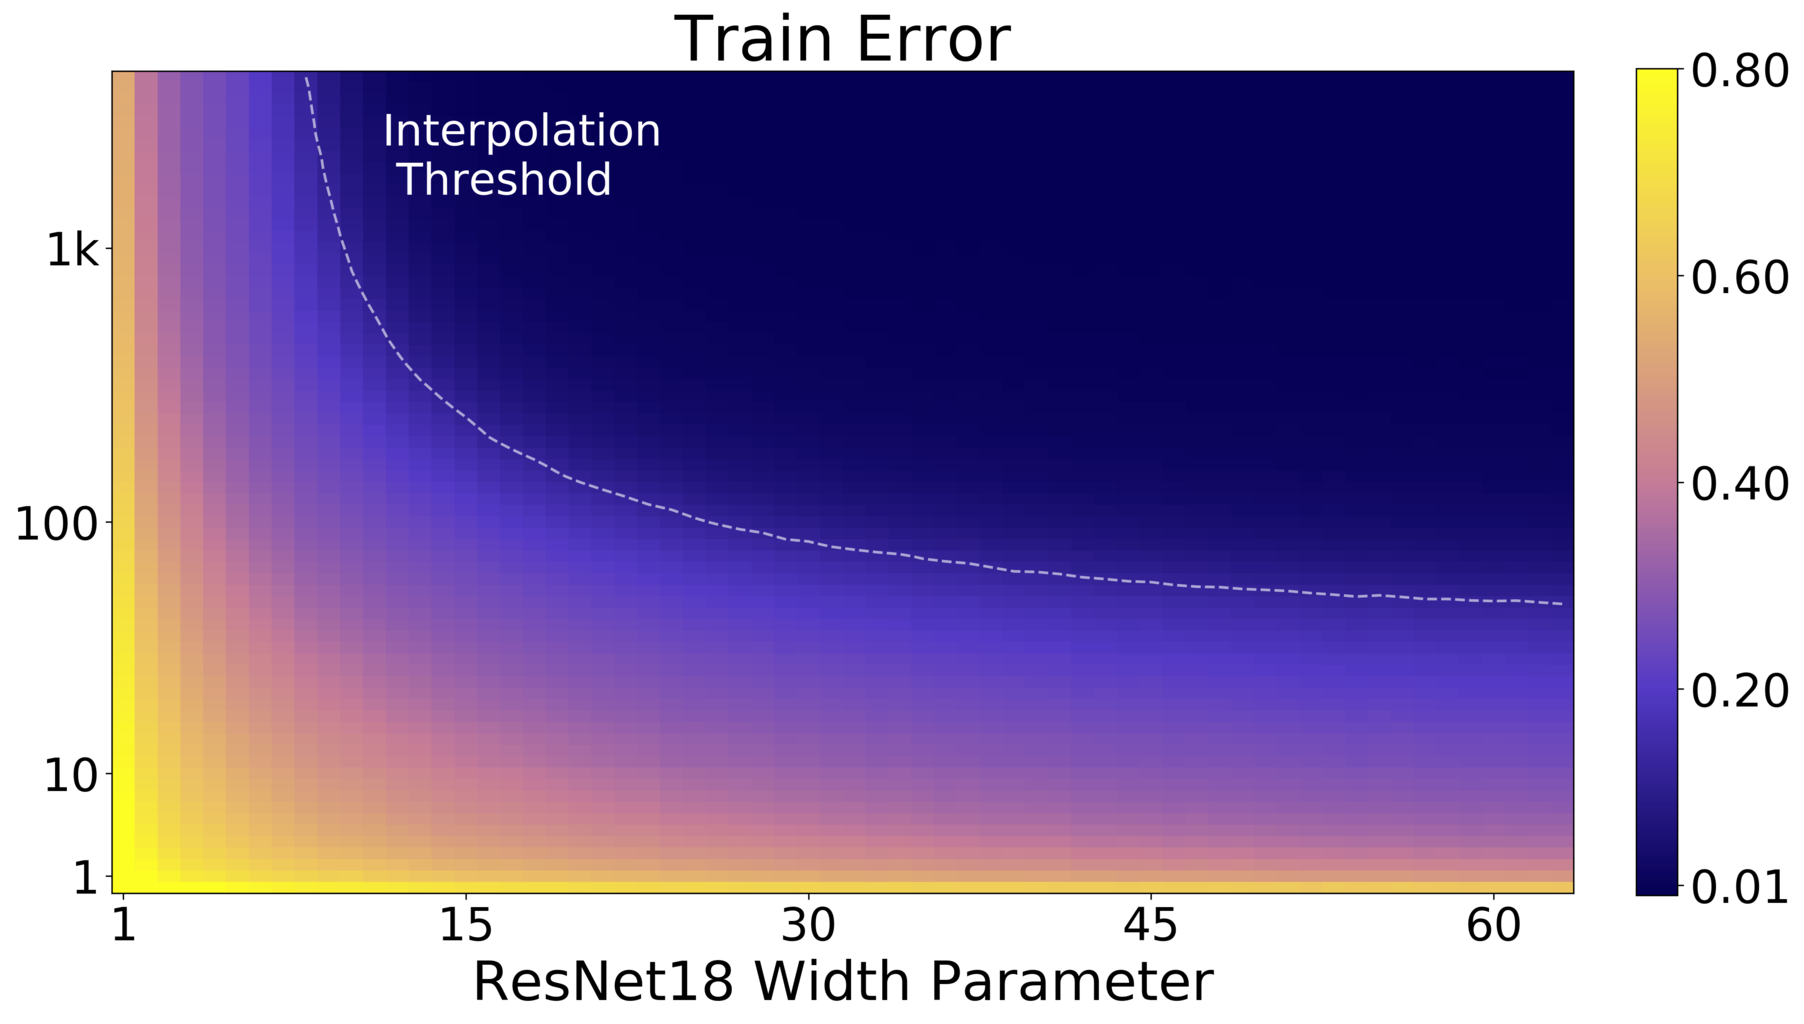
\includegraphics[width=1\textwidth]{media/Rn-cifar10-p15-adam-aug-train.png}
\end{minipage}
\caption{{\bf Left:} Test error as a function of model size and train epochs. The horizontal line corresponds to model-wise double descent--varying model size while training for as long as possible.
The vertical line corresponds to epoch-wise double descent,
with test error undergoing double-descent as train time increases.
{\bf Right} Train error of the corresponding models.
All models are Resnet18s trained on CIFAR-10 with 15\% label noise,
data-augmentation, and Adam for up to 4K epochs. Reused from \cite{nakkiran_deep_2019}}
\label{fig:unified}
\end{figure}

They define \emph{effective model complexity} of $\mathcal{T}$ (w.r.t. distribution $\mathcal D$) to be the maximum number of samples $n$ on which $\mathcal{T}$ achieves on average $\approx 0$ \emph{training error}. This is an entirely empirical definition, similarly per definition as VC-dimension. 

\newcommand{\EMC}{\mathrm{EMC}}
\begin{definition}[Effective Model Complexity]
The \emph{Effective Model Complexity} (EMC) of a training procedure $\cT$, with respect to distribution $\cD$ and parameter $\epsilon>0$,
is defined as:
\begin{align*}
    \EMC_{\cD,\eps}(\cT)
    :=  \max \left\{n ~|~ \E_{S \sim \cD^n}[ \mathrm{Error}_S( \cT( S )  ) ] \leq \eps \right\}
    \end{align*}
    where $\mathrm{Error}_S(M)$ is the mean error of model $M$ on train samples $S$.
\end{definition}

Using this definition, their main hypothesis can then be stated as the following three-fold regions:

\begin{hypothesis}[Generalized Double Descent hypothesis, informal] \label{hyp:informaldd}
For any natural data distribution $\cD$, neural-network-based training procedure $\cT$, and small $\epsilon>0$,
if we consider the task of predicting labels based on  $n$ samples from $\cD$ then:
\begin{description}
    \item[Under-parameterized regime.]  If~$\EMC_{\cD,\epsilon}(\cT)$ is sufficiently smaller than $n$, any perturbation of $\cT$ that increases its effective complexity will decrease the test error.
    \item[Over-parameterized regime.] If $\EMC_{\cD,\epsilon}(\cT)$ is sufficiently larger than $n$,
    any perturbation of $\cT$ that increases its effective complexity will decrease the test error.
    
    \item[Critically parameterized regime.] If $\EMC_{\cD,\epsilon}(\cT) \approx n$, then
    a perturbation of $\cT$ that increases its effective complexity
    might decrease {\bf or increase} the test error.
\end{description}
\end{hypothesis}

It is to notice that this definition is also only observational. By that, it only outlines the specific region of interest where the paradigm shift is identified through experimental results. It has no effective predictive power, or rather descriptive power more than setting up hypothesis with respect to the effective model complexity, and some arbitrary perturbation. \cite{nakkiran_deep_2019} also noticed this difficulty in providing a theoretical definition and theorem regarding such hypothesis, as said in their manuscript. The existence of the critical regime is also not defined. 

The behaviour itself has been particularly investigated, in certain settings. For example, before \cite{belkin_reconciling_2019}, \cite{advani2017highdimensionaldynamicsgeneralizationerror} investigated the generalization error in neural networks of high-dimensional measure. Of such, various behaviours that bear similarity to double descent can be observed. \cite{belkin2018understanddeeplearningneed} expanded on his previous research on the particular subset of kernel learning models, providing a theoretical analysis of specifically the Laplacian kernel on standard neural network. \cite{mei2020generalizationerrorrandomfeatures} investigated random feature regression in such regard, and also found similar results. 

The fact that double descent is not well-defined itself is a problem on its own. Up to the author's knowledge and of myself, there has been no effective definition or given description that outlines specifically how double descent can be structured. Instability in reproducing experiments and the effective range of the phenomena remains a question on its own. 

\subsection{So, what's the point?}
In the end of such introduction, what's the problem then? The problem comes from the way that bias-variance tradeoff principle is in itself - a \textit{principle}. The chain of responsibility that form the principle is very far away of the precursor shape of machine learning - we are talking about 1992 where the principle was first observed, is long. This includes empirical learning theory, model selection criteria, structural analysis and bounds of complexity-error, principle-based analysis and assumptions, theories and others that used to be considered universal of either intuition of mathematical proof (obviously with strong assumptions and setting), and vice versa coming up to even error measuring theory of learning process, and the learning process itself. Even then, certain sources (\cite{neal2019biasvariancetradeofftextbooksneed}) indicates even then inconsistency within the prediction of bias-variance tradeoff. It also indicates that certainly, there are something wrong with this, and certainly can be similar to how Newtonian mechanics is only the loose approximation up to certain range of effect, aside from macroscopically large (relativity) and astronomically small (quantum theory). It might as well be the same here. 

So, at this point, what can we do to solve this problem? Well\dots first, let us see what is the issue that we face beforehand then devise a plan to solve them. After all, without plan, we would be walking in totally blind - not saying that we are not already blind, just wiser of the path. 

\subsection{Problems}
There are a lot of problems regarding how we treat the problem, how we see it, and how we actively analyze it. Most of them lies in the space of statistical learning theory, since bias-variance on itself has variations and justification that is seemingly very natural in statistical theory, like the other version name \textit{approximation-estimation error tradeoff}. All of them contribute somewhat to the current outlook, and so far, it has been pretty bad, than what is being advocated of. Nevertheless, let us state them out, even if missing some particular details. 

\subsubsection*{Problem 1. Authoritative statements}
Despite its prevalence in particular research interest, double descent itself has no definite statement to describe its particular behaviour. This is also true for a list of other phenomena, such as \textit{grokking} (\cite{power2022grokkinggeneralizationoverfittingsmall}), \textit{emergence behaviours} (\cite{wei2022emergentabilitieslargelanguage}, typically discussed in large language models, which is understandable of large-scale specific ruling system), \textit{implicit bias} (\cite{soudry2024implicitbiasgradientdescent}), and \textit{neural scaling law} (\cite{kaplan2020scalinglawsneurallanguage,wei2022emergentabilitieslargelanguage}). There is also \textit{catastrophic forgetting} (\cite{vandeven2024continuallearningcatastrophicforgetting}) which is still fairly native of large systems; nevertheless, those phenomena will be of target later on (or discussed in later chapters). The fact remains that we only \textit{partially understand} these particular results with conjectures and theories to support the facilitation of new insights, new analytical lens, and nothing much. Without a clear definition of what is even double descent, sometimes, we cannot proceed, lest to say even solving it. This is particularly troublesome, since the current theory is so messy and not rigid that many even turns to exotic choices, like topological informatics learning theory, \textit{Homotopy Theoretic and Categorical Models} (\cite{Manin_2024}), and several more. So this is definitely one of the main problem to pushback on. 

\subsubsection*{Problem 2. Model complexity}
The notion of model complexity can be said to be often not so well-defined. There are attempts by \cite{hu2021modelcomplexitydeeplearning,luo2024investigatingimpactmodelcomplexity,barceló2020modelinterpretabilitylenscomputational,Molnar_2020,janik2021complexitydeepneuralnetworks}. The problem of model complexity is not so apparent until the inherent complex nature of models, typically in deep learning models (based on the MLP architecture) is observed to cannot be treated in similar way as classical models. In \cite{hu2021modelcomplexitydeeplearning}, most deep learning models are based on, and investigated of their complexity through measures like the expressive capacity, the effective capacity, and so on; aside from other teams and researchers investigated it by using computational complexity, or functional decomposition. One promising aspect of this is \cite{Molnar_2020}, where we are able to decompose the functional form a specific model into variations of its complexity. 

Nevertheless, it is reasonable to say there are no conclusive measure or definition of a model's complexity. Considering that double descent also appears outside the range of deep learning model, and is somehow consistent in classical models (for example in models tested by \cite{belkin_reconciling_2019}). This is particularly troublesome, as a theoretical analysis requires such definition, especially when the relation of interest is directly involved in such manner. This is a particular aspect needed to be resolved if there are to be progress made in this investigation. Additionally, the concept of overparameterization and underparameterization is also a problem, especially since its definition is not well-defined, hence become a problem in analysis by identifying the classification of the problem setting. 
\subsubsection*{Problem 3. Model structure}

In modern practice, the theoretical and formal treatment, rigorous consideration of different model structures and complexity is not realized. Partially, this is due to the bloom of machine learning and artificial intelligence from the early 2000s. Currently, there has been no conclusive theoretical definition or formulation about the structure of different models, typically can go under the name of mathematical modelling hypothesis, in a way that unify certain properties between architectures. Heuristics are also often employed in several newer models and widely-utilized structures typically seen in large-scale systems, leading to difficulty in formalization and factorization of affectants. 

\subsubsection*{Problem 4. Theoretical insufficiency}

The setting surrounding the learning theory, machine learning models is generally missing of its rigours and analytical properties. Most of the learning setting and model's training-testing setting are often narrowly stated in theoretical sense, and there are a lot of diffusing details that might or might not affect the model's perturbation without knowing. This in a certain way leads to the complexity in analysing different problem setting and experimental results, since the architecture used, the setting considered, model in questions, configuration (either custom or on system side) are not consistent overall. 

Furthermore, a lot of terms, definitions are often hand-waived in papers or in discussions. This also led to the point that in \cite{nakkiran_deep_2019}, they have to somehow 'reinvent' another type of model complexity itself, albeit unsatisfying of a definition, is still a new kind of definition per insufficiently of such. while it is welcome to introduce new definitions, the fact is that it is subjectively inconclusive of terms, definitions and thereof leads to the perception and situation where multiple studies can be found, but all of them are defined on different ground.

Analysing statistical learning theory and overall landscape of statistical learning theory, and the learning theory as a whole, encountering new problems like double descent also revealed its weakness, and ultimately, perhaps one of the reason why it is ineffective against such problem. First, there are simply too many assumptions made, too many formulations made during said process. Furthermore, there are also unclear notions and concepts, of which make it even harder to analyse or fully formalize. Secondly, there are inherent conflicts and uncertainty within those theories, formulations and notions by itself. For example, in one sense, the No-free-lunch theorem is considered to be representative and true, whilst also simultaneously being considered the opposite of such. And amidst abnormality behaviours of the old bias-variance formulation, we also find distinctive weakness in our theory, for example, the concerning difficulty in defining the notion of \textit{model complexity} in various contextual ways. To analyse double descent, perhaps we also need a new theory or formulation to support it. \footnote{Furthermore, most of the general solution and bounds created by statistical learning theory is often in a very simplistic system. For example, if we are to utilize the Rademacher complexity measure (\cite{10.5555/2371238}), most of the time we will have to compute it through the growth function $\Pi_{\mathcal{H}}(m)$ for $m$ points, on the standard finite hypothesis class $\mathcal{H}$ such that 
\begin{equation}
    \Pi_{\mathcal{H}}(m) = \max_{x_1, \dots, x_m \in \mathcal{X}} \left| \left\{ (h(x_1), \dots, h(x_m)) \mid h \in \mathcal{H} \right\} \right|
\end{equation}
Most of our problems resolve to binary classification, or rather, the problem of pattern recognizing discrete, reduced classification form. It is not so sure for now if all problems can be reduced to such way, so we cannot draw conclusive analysis that is not diluted of mathematical formulation for complex systems. That is not to count the computationally intensive operation required to calculate the supposedly classical measure, while not entirely of itself holds any substantial reasonable information about the internal dynamics of the model itself. }

Another problem with classical analytical solution is that it is very \textit{loose}, almost too loose to even considered of such. But sometimes it is too \textit{rigid} in a sense such that it simply does not work at all. Indeed, basing our works and foundational assumptions on top of approximation theory is not quite good at all, because they are very limited. Overall, we can say it is not equipped for handling similar situation. For example, almost all bounds that is subjected of classical learning theory only guarantee particular existential theorem, under very simplified and specific situation without the virtue of extending it to a more general setting. 

This is particular event or rather pattern that we often see in learning theory development, or machine learning theory in general - the `\textbf{mathification}' of a theory. Even though we need mathematics on either end, the approach is impractical or simply wrong, believing mathematics to be the singular thing that defines learning theory. This has many fallacies that can then be attributed to a lot of factors and whatnot, of several factors that plague this analysis even further than just the problem of double descent. For now, 
\begin{enumerate}[itemsep=2pt,topsep=1pt]
    \item Epistemological limits and interpretations (\cite{electronics13020416}) - We ultimately lack understanding of a lot of things. While those `theorems' are very nice in learning theory, the real picture is that it is not real learning, for the word learning are not even defined, as such is to compare them to \textit{human learning} on itself. Even by then, theorems are severely limited. Certain voices also concern of similar problem, including \cite{lipton2016mythos,doshi2017towards,molnar2020general} (\cite{molnar2020general} shortly consider the misleading interpretation question instead), and philosophically, with several pushbacks on structural anecdotes, \cite{dreyfus1965alchemy,dreyfus1972what,dreyfus1986mind,suchman1987plans,brooks1991intelligence,searle1980minds,mccarthy1969philosophical,harnad1990symbol}. On the more modern side, of contemporary critiques, \cite{pearl2009causality,marcus2018deep,sutton2019bitter}. Of the Chinese Room Argument, perhaps we can look into already copulated passages. 
    \item Applying wrongly, and is used to impress and not to explain anything (\cite{lipton2018troublingtrendsmachinelearning}) - mathematics is used to \textit{impress} certain demographic of reviewers and readers, to provide a sense of rigours, to further enhancing the image of formal theory to the point that such theory, even if wrong, can be considered fairly correct by the sheer volume of practitioners believing in such. Such is to say the \textit{mathiness} is turning things into ideology more than rigours itself, of which we can take a tangent to see in economic theory, one of the place to adopt a large portion of machine learning statistics, the pushback against such cursed devolution (\cite{romer2015mathiness,syll2024postreal}). 
    \item Reproducibility and acute false claims (\cite{kapoor2022leakage}) - In general, what we have done cannot be recreated, in certain way, and of certain too optimistic setting that is seemingly unrealistic - particularly in adoption toward practical means of actions. 
\end{enumerate}
While most of those are not directly related to our problem - suffice to say the general narrative is so, it particularly indicates a very serious error in the theoretical development itself, and the scope of its reach has been perhaps confirmed at hand. Attempts to solve this problem might need to be an entirely new framework, of something that unify the theory at-hand, or by relinquished attendances to the current dilemma using old and trusted foundation, yet will inevitably fail to resolve further outcome of the solution since its onset is beyond the classical theory. Such is to say, we need an entire solution to cover this particular track. One is promising of them all, being the \textit{Neural Tangent Kernel} (\cite{Jacot:2018:NTK}), but other than that, nothing much came through. 

\section{Classical attempts}

Nevertheless of me and people saying (more like only me) that the problem require new theories entirely, we can at least work something out of the current status quo, if you might or might not believe so, at least before observation. Thereby, let's get into it and see what can we do, given the current knowledge, albeit messy it is. 

Identifying the problem, we can see that we are lacking the analysis on the component that makes up the theoretical assumption of bias-variance tradeoff. Thereby, one of the main problems would be to inspect such term. Next, bias-variance tradeoff makes use of certain assumptions on the learning setting and bounds in their statement of convergence, of an algorithm $\mathcal{A}$, and also \textit{complexity measure on hypothesis $h\in\mathcal{H}$}. Those are what we have to address, alongside with already existing partial solutions and analytical results from other researchers. 

\subsection{Observing gradient of decompositions}

While the interpretation of what the bias-variance tradeoff, the usual training-versus-test curve, and statistical learning consideration, another interesting aspect to consider (as well for double descent), is how bias-variance decomposition acts on gradient descent and its components. This claim is perhaps reinforced by the work of \cite{adlam2020understandingdoubledescentrequires} which indicates that different bias-variance decompositions effects differently on the total system mechanism. 

The main term of a gradient descent algorithm is the gradient of the loss function $\mathcal{L}(h(x),y)$. For the hypothesis $h$, the number of instances supplied denoted by $k$ has three main cases: $k=1$ for stochastic descent, $k\in (1,m)$ for batch gradient descent, and $k=m$ for standard gradient descent, for a given space of $m$ samples. The gradient in such case is calculated using the empirical risk on $m$ size, that is: 
\begin{equation}
    \mathcal{L}_{k}(h(x),y) = \hat{R}_{S[k]}(h) = \frac{1}{k} \sum^{k}_{i=1} \ell(h(x_{i}),y_{i})
\end{equation}
We use the classical bias-variance tradeoff at first. Since the gradient is a linear operator, we have: 
\begin{equation}
    \begin{split}
        \nabla_{k}(\mathcal{L}) &= \nabla_{k}\left(\pa{\E\hat{y}(\bfx) - \E y(\bfx)}^2 + \V\qa{\hat{y}(\bfx)} + \V\q{y(\bfx)}\right)\\
        & = \nabla_{k}\left( \E\left[\hat{y}(\bfx)\right] - \E\left[y(\bfx)\right] \right)^2 + \nabla_{k}\V\left[\hat{y}(\bfx)\right] + \nabla_{k}\V\left[y(\bfx)\right] \\
        & = \nabla_{k}\left( \E\left[\hat{y}(\bfx)\right] - \E\left[y(\bfx)\right] \right)^2 + \nabla_{k}\V\left[y(\bfx)\right]
    \end{split}
\end{equation}
This effectively decompose the gradient into three parts that influence the overall gradient calculation. Because $\nabla_{k}\V\left[y(\bfx)\right]$ calculates the gradient of irreducible error, which is supposed to be constant of the sample space, it is then equal $0$. Suppose a sample $\mathbf{x}_{k}$ of size $km$, of partition $k$. Hence, we have gradient descent based on $k$th run over the entire dataset, permuted. Then, the loss function calculates in the form 
\begin{equation}
  \nabla_{k,n}(\mathcal{L}) = \nabla_{k,n}\left[ \frac{1}{n}\sum_{i\leq n} \hat{y}(x_{kn+i})  - \frac{1}{n}\sum_{i\leq n} y(x_{kn+i}) \right]^{2} + \nabla_{k,n} \left[ \frac{1}{n}\sum_{i=1}^n y(x_i)^2 - \left( \frac{1}{n}\sum_{i=1}^n y(x_i) \right)^2 \right]
\end{equation}
The indices is now changed to $(k,n)$ for $m/k=n$ as the $i$th partitioned, ordered run, thereby $kn+i$ runs for the index. If we assume a simplified structure $\theta_{t}$ of parameters $y(x_{i})$ depends on, we can reduce it further.  
\begin{align}
\nabla_{k,n}(\mathcal{L})
&= 2\left(\frac{1}{n}\sum_{i\le n}\hat{y}(x_{kn+i}) - \frac{1}{n}\sum_{i\le n}y(x_{kn+i})\right)
   \left(\frac{1}{n}\sum_{i\le n}\nabla_k\hat{y}(x_{kn+i}) - \frac{1}{n}\sum_{i\le n}\nabla_k y(x_{kn+i})\right) \\
&+ \frac{2}{n}\sum_{i=1}^n y(x_i)\nabla_k y(x_i)
   - \frac{2}{n^2}\left(\sum_{i=1}^n y(x_i)\right)\left(\sum_{i=1}^n \nabla_k y(x_i)\right)\\
   & = = 2 \left(
   \left( \mathbb{E}_n[\hat{Y}] - \mathbb{E}_n[Y] \right)
   \left( \mathbb{E}_n[\hat{G}_k] - \mathbb{E}_n[G_k] \right)
   + \mathbb{E}_n[Y G_k] - \mathbb{E}_n[Y] \,\mathbb{E}_n[G_k]
\right)\\
&= 2 \left( 
   \left( \mathbb{E}_n[\hat{Y}] - \mathbb{E}_n[Y] \right)
   \left( \mathbb{E}_n[\nabla_k \hat{Y}] - \mathbb{E}_n[\nabla_k Y] \right)
   + \mathrm{Cov}_n\!\left(Y, \nabla_k Y\right)
\right) \\
& = 2 
   \left( \mathbb{E}_n[\hat{Y}] - \mathbb{E}_n[Y] \right)
   \left( \mathbb{E}_n[\nabla_k \hat{Y}] - \mathbb{E}_n[\nabla_k Y] \right) + 2\mathrm{Cov}_n\!\left(Y, \nabla_k Y\right)
\end{align}
for 
\begin{equation}
    \mathbb{E}_n[Z] = \frac{1}{n} \sum_{i=1}^n Z_i,
\qquad
\mathrm{Cov}_n(U,V) = \mathbb{E}_n[UV] - \mathbb{E}_n[U] \,\mathbb{E}_n[V].
\end{equation}
Here, we can see two terms multiplication, for the first one being the correlation between the expected error $\mathbb{E}_n[\hat{Y}] - \mathbb{E}_n[Y]$ and the gradient $\mathbb{E}_n[\nabla_k \hat{Y}] - \mathbb{E}_n[\nabla_k Y]$. This measures the correlation between the expected error, and the gradient measure. The second term is exactly the empirical covariance between the target $Y$ and the true gradient component. Since we are taking a fixed concept case, we can simply disregard the truth gradient hence $\mathbb{E}_n[\nabla_k Y]$, for which the term is reduced to $2\left( \mathbb{E}_n[\hat{Y}] - \mathbb{E}_n[Y] \right) \left( \mathbb{E}_n[\nabla_k \hat{Y}] \right)$. Under this same assumption applied to the covariance term, we obtain
\begin{equation}
    \nabla_{k,n}(\mathcal{L})
= \frac{2}{n}\sum_{i=1}^n \big(\hat Y_i - Y_i\big)\,\partial_k \hat Y_i = 2\left(
   \left( \mathbb{E}_n[\hat{Y}] - \mathbb{E}_n[Y] \right)
   \mathbb{E}_n[\nabla_k \hat{Y}]
\right)
\end{equation}
Looking into some particular algebraic representation, we can write this simply as
\begin{align}
    \nabla_{k,n}\mathcal{L}
    &= 2\,\mathbb{E}_n\!\left[(\hat Y - Y)\,\nabla_k \hat Y\right] \\
    &= 2\Bigg(
    \underset{\left[\mathbb{B}(\hat{Y},Y)\right]^{1/2}}{\underbrace{\bigl(\mathbb{E}_n[\hat Y] - \mathbb{E}_n[Y]\bigr)}}\,\mathbb{E}_n[\nabla_k \hat Y]
    + \underset{\mathrm{Cov}_n(\hat Y,\,\nabla_k \hat Y)}{\underbrace{\mathbb{E}_n[\hat Y\,\nabla_k \hat Y] - \mathbb{E}_n[\hat Y]\,\mathbb{E}_n[\nabla_k \hat Y]}}
     \\
    & \quad \quad \quad \quad \quad -\underset{\mathrm{Cov}_n(Y,\,\nabla_k \hat Y)}{\underbrace{\mathbb{E}_n[Y\,\nabla_k \hat Y] - \mathbb{E}_n[Y]\,\mathbb{E}_n[\nabla_k \hat Y]}}
    \Bigg)
\end{align}

The first term can be attributed to self-correct of bias-error gradient correlation, while the two covariance term suggests correlation between model randomness and its gradient, and the last one deal with the truth-gradient correlation. What those gradients mean will have to be tested in some preliminary models. Generally, we should not expect the result to be quite effective. Similar decomposition can be conducted for the other decomposition, as suggested, however, the gradient effect is particularly interesting, and will have to be resolved. Let's see what we can do. 



\subsubsection{Modern bias-variance decomposition}

We are not entitled to decompose error measure to the exact final terms of bias-variance decomposition where the bias and variance is totally available. There are certainly different way to do this, as classified in \cite{adlam2020understandingdoubledescentrequires} paper. Some of this are particularly specialized in \textit{neural network} training. 
\begin{enumerate}[leftmargin=1cm,itemsep=2pt,topsep=1pt]
    \item \textbf{Semiclassical approach}: The semiclassical approach is fairly simple. We can rewrite to another variation of the classical approach to be \begin{equation}
        \underset{h\in\mathcal{H}}{\mathbb{E}[\ell(h)]} = \mathbb{E}_{x}\mathbb{E}_{\epsilon}\left[\hat{y}(x)-y(x)\right]^{2} = \mathbb{E}_{x}\left(\mathbb{E}_{\epsilon}[\hat{y}(x)]-y(x)\right)^{2} + \mathbb{E}_{x}\mathbb{V}_{\epsilon}\left[\hat{y}(x)\right]  
    \end{equation}
    and instead, consider the \textit{structural conformation} of the decomposition, or rather, taking the expectation within $\theta\in \Theta$ of the structural description of $h\in\mathcal{H}$. Then, we shall have 
    \begin{equation}
        \underset{h\in\mathcal{H}}{\mathbb{E}_{\mathrm{SC}}[\ell(h)]} = \mathbb{E}_{x}\mathbb{E}_{\theta}\mathbb{E}_{\epsilon}\left[\hat{y}(x)-y(x)\right]^{2} = \mathbb{E}_{x}\mathbb{E}_{\theta}\left(\mathbb{E}_{\epsilon}[\hat{y}(x)]-y(x)\right)^{2} + \mathbb{E}_{x}\mathbb{E}_{\theta}\mathbb{V}_{\epsilon}\left[\hat{y}(x)\right]
    \end{equation}
    Do note that the order matters, since the expectation can be constant of a given ordering. And expected value over constant is just the constant. 
    \item \textbf{Symmetric decomposition}: This approach is fairly difficult, we refer to the paper itself of its own justification on the decomposition. The symmetric decomposition relies on the shape of the input, $\mathcal{X}=\{P,D,\epsilon\}$, of which you can remove the $\epsilon$ term and retain some decomposition on $P$ and $D$ per distribution. 
\end{enumerate}
Such decomposition can be fairly hard to work out its gradient details, yet we might as well have to do it either way, since we are entrusted of targeting the over terms concretely in this direction. 

\subsection{Bounding inequalities}

We briefly mentioned classical learning theory in accordance to our analysis. In particularly, we would like to draw out the fundamental results that have been driving learning theory, and what they say beforehand of the analysis. Would it just only that the old theory being misrepresented, misinterpreted, or there exists some fundamental restriction of the theory that lead to bias-variance being considerate of such setting only, with certain strong assumptions that lies within the theory itself, and can be extended or removed toward generality. Such is to say quite a bold claim, but worth to consider pursuing it. 

In consideration of the PAC-ERM bound, of which restrict $R(h)$ and $\hat{R}(h)$ on some particular restriction, at least for ERM, they are fairly implicit in nature. We will have to reinterpret what they are saying to us, since it does not make much sense usually so. But the general pitfall that we have to be careful of usually lies in the nature of the bounds themselves. Specifically, their fame of being rather existential guarantees but no process-based analytic. 

The first point of approach comes from either the \textit{Probably Approximately Correct} framework and its variation (we would like to talk of the singular original framework) or the \textit{Vapnik-Chervonenkis} framework of learning guarantees. Both of them serve what is there to be called a learning bounds within finite hypothesis class, or by reduced optimization problem with estimators. PAC bounds typically guarantee the upper, worst-case scenario bounds, while VC-dimension of its own definition is typically used for general lower bounds. Nevertheless, we have to know how they work to interpret and use them correctly.

PAC-learning criteria started by specifying a restriction bound in which, the probability that the generalization error can be achieved, for error margin $\epsilon > 0$, is less than a confidence point of $1-\delta$ for $\delta > 0$. How they did this? Well, by bounding the error under specific $m$ samples of the observation space such that the above criteria is guaranteed, given $m\geq poly(1/\epsilon, 1/\delta, n,size(c))$ where $size(c)$ is the representation space of the concept to be learnt from, and $n$ is the input-dimension on itself. Basically, the guarantee under worst-case scenario, whether the generalization error evaluated of the algorithm $\mathcal{A}$ be specifically satisfying the criterion. This, is a \textit{concept-aware} criteria - reflected by specifying the general copula, restricting the algorithm and consider the term of the \textit{ambiance space} \footnote{In general notion, the ambiance space is what we called the \textit{object collection set}, containing the system's dynamical components and what to consider of itself. Basically, the $S$ in the mathematical modelling setting} $\mathbb{A}=(\mathcal{C},\mathbb{I}(n,m))$ upon the evaluator correspondence. The advantage of this method is well-known - it bounds, for example, for how many samples would it be possible to learn, under the assumption that the algorithm $\mathcal{A}$ can indeed, learn such that $h^{*}$ of the final result is $\inf_{h\in\mathcal{H}}\hat{R}(h)$, within polynomial expression of $m$. However, the implication of PAC-learning, is large and fairly difficult to attend to, such is to say they also consider the consistent and inconsistent case already, which is good, but still fairly not so straightforward in particular expression. 

For example, PAC-learning on ERM principle requires that, for some particular notion of the bounding method, such that the following bound will be true, 


\begin{proposition}\label{prop:PAC_ERM_1_recite}
    For any $h\in\mathcal{H}$, for any $\delta\in(0,1)$, 
    \begin{equation}
        \mathbb{P}_{S}\left( R(h) > \hat{R}(h)+ C\sqrt{\frac{\log{(1/\delta)}}{2n}}\right)\leq \delta
    \end{equation}
\end{proposition}

This bound works, under scrutiny assumption such that $c$ and $h$ effectively does not matter in such case, and only use the concentration inequalities on the estimated empirical error on loss function of a particular setting. This is by itself, not so rigorous, and not of the spirit of the PAC-learning boundary itself. The guarantee itself is, controversially, not even a good one. At least for our interest, it does not say anything about the algorithm, it does not say anything about the hypothesis internal mechanics (if the mechanistic model is exposed, like when the concept class is defined, usually, the hypothesis is supposed to work the same way, which is indeed, not the case). What we miss here, is a lot of those factors together. Nevertheless, the PAC-learning bound indicates a particular insight. We have to \textit{formalize} the instance/observational space; we will have to formalize, of it, the sample $m$, the dimension of the encoding $n$, the representation system used by $size(c)$, the concept, and indeed, of the structure of the hypothesis space $\mathcal{H}$ of which gives detail to the hypothesis itself. Such is to say, we need to somehow make the PAC-criteria to be \textit{structural-aware}, per meaning of the word. 

For VC-theory and the concept of its dimension, its limit is again, well-known up to certain accordance. Classical VC-theory worked upon a fairly restricted, discrete framework of classification, usually binary classification (for SVM) for example, on \textit{shatterable concept space}. The more, fairly advanced version of \textit{fat-shattering} and multiclass-VC domain still fall short of the generality and more complex structure - in which case we mean the simpler the restriction on what the task is. Insights and ideas toward VC-theory is rather explicit of its own principle - fundamentally speaking, VC-theory conjure to the \textit{combinatorial VC-dimension} of all possible solvable system, up to certain data points, of certain class, except of special cases. Such is to say that one of the aspect that Vapnik-Chervonenkis theory focus on is one particular \textit{expressive complexity} of a specific model. This is also a problem that we have to solve. 

Classical Rademacher is also very hard to justify of its use here. Classical Rademacher analysis typically refers to the application of \textit{Rademacher complexity}, a near-empirical theoretical definition of complexity class. One advantage that it poses, against VC and PAC-based structures, is that the ambiance space of Rademacher complexity is not restricted toward particular class of problem, like binary labelling of the other theoretical analysis. Nevertheless, Rademacher complexity is unstable (leading to its dilemma of having very few closed-form results) and computationally difficult. Its bounds are also of the same fate, lest to say some of the results proceeded of the Rademacher complexity are often refuted in empirical experiments. Furthermore, strong assumptions and restricted bound cases still hinders its usefulness. And best of all, it does not have anything reasonable analysis for complex structure other than the plain estimators. 

Those critiques against classical analysis is not alone of myself. Rather, there are indeed a lot of invoices on such matter toward new development of learning theory. Specifically so, \cite{zhang2017understandingdeeplearningrequires} inquired of the fact that bounds are often vacuous in terms of deriving for deep neural network. Of the same paper is also the opinion that expressivity is not generalization, which is, obviously true from our theoretical preliminary. \cite{truong2025rademachercomplexitybasedgeneralizationbounds} discussed the instability and hard computation of the Rademacher bound, also of threshold behaviours. On the core topic of generalization (which a lot of people pursue for obvious reason), \cite{nagarajan2021uniformconvergenceunableexplain} argued against the current uniform convergence theory that seemingly fail to garner an understanding of such behaviour, and so is \cite{tunali2019empirical}. Solutions exist, yes, but either in the form of partial solution and variation of classical theory, like PAC-Bayes, some way of experimenting, like \textit{stability-based analysis}, \textit{margin/norm measures} or localized Rademacher complexity \cite{bartlett2005local,bartlett2017spectrally,bousquet2002stability,neyshabur2015norm}, yet they are still as we said, \textit{partial of its form}, and no solution has emerged, yet. We would likely want ourselves to not follow the same path again. 

\subsection{Complexity notions}
Even though such can be said of the pitfall of current practices, it is still not the end of the road, or at least of the principle in which we apply to our empirical study - to force double descent out. Which is rather harder than what it looks like. We might as well attempt to analyse double descent in terms of classical, non-novel theory first, before jumping straight into conclusion without personal observations. First, the issue of bias-variance and double descent is related to multiple factors, but specifically between the notion of bias-variance and complexity-accuracy. However, their definition and usage in certain contexts are obscured, thus would require a fairly thorough consideration. Most of these results contains of bounds and often discussion of random processes, and also restricted itself to mathematically well-defined setting. For now, we would like to investigate their notions and applications. Though for starter, we have to discuss the following preliminary. The hypothesis class $\mathcal{H}$ has two types of classification: either infinite hypothesis class $\mathcal{H}^{\infty}$ or finite hypothesis class $\mathcal{H}^{n}$. Based on the details of the expression of representation strings (\cite{10.5555/200548}), an infinite hypothesis class contains infinitely many specifiers of the hypothesis structure. Note that this does not correlate to an increase in parameter, as we will see with the case of axis-aligned rectangle - for only four parameters $(l_{1},l_{2},h_{1},h_2)$ we can specify all axis-aligned rectangles with their value taken from the field $\mathbb{F}=\mathbb{R}$. Finite hypothesis class is then can be understood of the number of configuration, or in discrete form combinatorial pairs that can be presented of the hypothesis class, for example, a string of all $n$-length binary numbers $\{x_{1},\dots,x_{n}\}, x_{i}\in \{0,1\}$. A subtlety that would then have to discover, is the increment in size of the hypothesis to accommodate either finite or infinite number of specifying parameters - one example can be sampled from is the class of all support vector machine (SVM, \cite{Vapnik1999-VAPTNO}), which for now we treat it as it is. The concept class can then also be treated similarly. Here, we assume a setting where unless specified, we have knowledge of the concept class structures, but not the hypothesis. 

Assume the working space is the real field $\mathbb{R}^{n}$. Let us recall a model $h\in\mathcal{H}$ of certain hypothesis class $\mathcal{H}$. Then, the \textbf{complexity} refers to the complexity of the hypothesis $h$ itself; there is also the notion of class maximal complexity for $\mathcal{H}$. Complexity in this case refers to the mass of the model, or rather, to answer the following questions:
\begin{enumerate}[itemsep=0.5pt,topsep=0.5pt]
    \item What is the effective expression range of a hypothesis?
    \item What is the hypothesis structured in?
    \item If the model is constructed by parameters, how many parameters are there?
    \item How many components are there in specific model $h$, and how would another model $h'\in \mathcal{H}$ differs from $h$?
\end{enumerate}
Those questions are not so easily answered. Specifically, analysis often puts the hypothesis class $\mathcal{H}$ as a class of functions. So, there exists the class $\mathcal{H}_{n}$ of $n$-th degree polynomials, or else. Effective complexity in such case means the range of expression a function can give - for example, for $n$-th polynomial class, we already have the Weierstrass's theorem that tells us that any continuous function of closed interval can be approximated by a polynomial of arbitrary order. These expressions depend on the field or space the hypothesis class lives in, for example, if the hypothesis is configured to work in the set of all functions in $\mathbb{F}=\mathbb{R}$ of algebraic field, then we call it the algebraic family. There are various hypothesis classes in such case, and usually, not a lot of them can be analysed and represented in the same way, and hence also the analysis of the `size' of the hypothesis, also between different hypothesis classes. This prompted the usage of a more general notion, called \textbf{representation complexity}. Representation complexity refers to the number of components needed to express $h$ and generally, any hypothesis in $\mathcal{H}$. This is often the parameters count, since the parameters themselves are used in constructing the function in algebraic system. Thus, again, an $n$-th degree polynomial might have $2(n+1)$ parameters, for $n+1$ variational input (or variable), and $n+1$ coefficients. Notice that we specifically at the beginning, use the notion of algebraic structure $\mathbb{R}$ because of it. If we restrict ourselves to the expression, for example, for $\mathbb{B}=\{0,1\}$, then it can be expressed in various ways in logic theory, such as conjunctive normal form (CNF), disjunctive normal form (DNF), and else. This forbid the analysis based on the effective process itself, but rather the number of components required, hence taking them as complexity of construction. 

Furthermore, the above two measures only talk about the \textbf{general mass} (representation) and \textbf{general expression}. In a deeper analysis, we haven't talked about the general individual complexity of the model itself. This notion refers to the complexity computed or evaluated, by considering the process-dependent behaviours and range of a specific expression influence on the operational process itself. While expressive complexity can provide a sufficient bound of approximation strength, the individual strength that can make it happen (for example, the fact that $n^{k}$ value range versus $n^{k-1}$ value range is totally different by one power degree), the contribution and sum of individual components can only be discussed using the general individual complexity, by using \textbf{process complexity} term. Up until now, this has not been formulated as author's knowledge, hence the two standard term would then be used instead in the analysis. 

\begin{table}[htbp]
  \centering
  \footnotesize
  \begin{threeparttable}
    \caption{Descriptions of complexity measures applied to models and learning processes}
    \label{tab:complexity-measures}
    % three columns: adaptive widths
    \begin{tabularx}{\textwidth}{@{} >{\RaggedRight\arraybackslash}X
                                     >{\RaggedRight\arraybackslash}X
                                     >{\RaggedRight\arraybackslash}X @{}}
      \toprule
      \textbf{Measure} & \textbf{Purpose} & \textbf{Remarks / Scope} \\
      \midrule
      Representation complexity
        & Complexity of encoding a model (size of representation, alphabet-dependent).
        & Model-level measure; depends on chosen encoding/representation and can be used to quantify storage or description length. \\
      \addlinespace[2pt]
      Expressive complexity
        & Complexity of the model's observable behaviour (operational expressivity of the mapping it implements).
        & Model-level; measures the variety of input–output behaviors the model can implement. \\
      \addlinespace[2pt]
      Structural complexity
        & Complexity of the model's internal architecture (how components compose and interact).
        & Decomposable into component-wise measures (e.g., per-layer, per-module) and useful for architectural comparisons. \\
      \addlinespace[2pt]
      Structural mass
        & Aggregate representation size derived from representation complexity across the model.
        & Global model measure for total encoded size (e.g., total parameter encoding length). \\
      \addlinespace[2pt]
      Sample complexity
        & Number of samples required to reach a prescribed performance level (statistical sample-count).
        & Process-level measure; depends on hypothesis class, loss, and desired error/confidence. \\
      \addlinespace[2pt]
      Sample space complexity
        & Intrinsic complexity of the data distribution / sample domain (richness, diversity, structured-ness).
        & Statistical measure over the sample space; affects learnability and effective sample size. \\
      \addlinespace[2pt]
      Optimization complexity
        & Complexity of the learning algorithm (convergence rate, computational/iteration cost, sensitivity).
        & Process-level; hard to pin down analytically, often characterized empirically or by worst-case bounds. \\
      \bottomrule
    \end{tabularx}

    \begin{tablenotes}
      \footnotesize
      \item[] \textbf{Notes:} The notion of structural mass is convoluted. In certain setting, it is simply the parameter space $\theta\in\Theta$, but in some setting, there exists fundamental difference than identically weighted parameter space complexity, as seen in multi-basis polynomial models, not taking into account homogeneous deep learning networks. Optimization complexity coincides with PAC-learning bounds for polynomial runtime, and \textit{sample complexity} sometimes can only be the dimension of the input/observation space.
    \end{tablenotes}
  \end{threeparttable}
\end{table}

The above complexity, aside from sample space-related measure, can also be applied onto the concept class's members itself. We also take the class complexity in such case, as the argument that maximize those measure: that is, the largest value of the measure, taken on the class as the class's complexity. 

The next complexity measures that can be taken of, comes from the learning process structure itself. Usually, in statistical learning theory (\cite{STL_Hajek_Maxim_2021,10.5555/2371238,10.5555/2621980}), we often use the setting that is related to \textbf{supervised process}. This usually means the process can be configured in a feedback loop, or induced response toward the model - often come from the observational space, where the concept that is set to be the target of the process - then called as learning process - is conjured. For now, we reserve this to the classical learning theory and process, and will not inquire further of such direction. 

The learning process assumes an operational space containing the structure, for example, $\mathbb{R}$-encoding space of real values, and a set of \textbf{samples} living in such space, denoted $\mathcal{S}$. Those samples are often referred to as the \textbf{observation set} of a particular objective of learning. As mentioned above, $\mathcal{S}$ belongs to the concept $c$, assumed to be of certain concept class $\mathcal{C}$. $\mathcal{S}$ is obtained by using an observing process to create or generate the result. This process can be determined or considered in multiple way, however, generally can be considered by having a deterministic interpretation (using an explicit function $c(x)$) or by probabilistic approach (modelling a distribution $\mathcal{D}$). Hence, we gain another type of complexity, with regard to the process called \textbf{sample complexity} - usually defined of cardinality - the amount of sample needed for particular purpose, for particular objective. For the complexity category up to the structure of the learning setting by itself, we call it the \textbf{sample space complexity}. 

One final complexity that is worth mentioning is then the \textbf{optimization complexity}, measure on the action of the learning algorithm. By such, it investigates the construction of an optimization algorithm solely dependent on its size of the algorithm, and other non-process related measures. Optimization complexity can also be related or expressed, in situation of time complexity, which is typical in computing system. 

\subsubsection{Representation complexity}

Representation complexity works in assumption of the wider concept class $c\in \mathcal{C}$. However, it can also be applied onto the hypothesis class $\mathcal{H}$. To define it however, we need to define the concept of a representation scheme (\cite{10.5555/200548}). 

\begin{definition}[Representation scheme]
    For a given concept class $\mathcal{C}$, a \textbf{representation scheme} for such concept class is a function $\mathcal{R}: \Sigma^{*}\to \mathcal{C}$, where $\Sigma$ is the finite alphabet of symbols. We call any configuration $\sigma \in \Sigma^{*}$ such that $\mathcal{R}(\sigma)=c$ a \textbf{representation} of $c$, under $\mathcal{R}$. For any given $c$, the representation scheme might not be unique. \footnote{Perhaps representation scheme can be further realized by applying a Borel $\sigma$-algebra on top, and put on it a perspective measure to handle the notion of representation size. For example, in the traditional example of axis-aligned rectangle, one such representation scheme could be the real number schema $\mathcal{R}:(\Sigma \cup \mathbb{R})^{*}\to \mathcal{C}$, which then can utilize the extended notion of a Lebesgue measure over $\mathbb{R}$ and its spaces.}
\end{definition} 

The representation of a specific concept or hypothesis classes can be different. Consider the learning problem of a Boolean string. The representation can take form as the \textbf{conjunctive normal form} (CNF) or \textbf{disjunctive normal form} (DNF), with their expressiveness on equal, however string length varies exponentially, as seen by \cite{Wegener1987,MiltersenRadhakrishnanWegener2005,DarwicheMarquis2002}. Since the learning algorithm has access only to the input-output behaviour of $c$, in the worst case, it must assume that the simplest possible mechanism is generating this behaviour. Within this assumption, we can now formulate the \textbf{representation size} or \textbf{representation complexity} of particular concept, denoted $size(c)$. 
\begin{definition}[Representation complexity]
    Given a concept $c\in\mathcal{C}$, the \textbf{representation complexity} of $c$ is defined to be the size of the smallest representation of the concept $c$ in the underlying representation scheme $\mathcal{R}$, that is, 
    \begin{equation*}
    size(c) = \min_{\mathcal{R}(\sigma)=c}\{size(\sigma)\}
\end{equation*}
for any string $\sigma$ of the representation scheme $\mathcal{R}$ that still represents $c$.
\end{definition}
Under such definition, the more "complex" the concept $c$ is with the respective chosen representation scheme, the larger $size(c)$ is. This is also where the concept of the concept class $\mathcal{C}$ comes from - it comes from the \textit{representation class indiction} that we have in mind some fixed concept classes we study by their representation scheme. We note that, however, the definition works within the least-lower bound limit - we choose the infimum. In the worst-case scenario, the representation potential mismatch between $h$ and $c$ might be very large, hence the \textit{effective representation} might not be the same. We also operate on the assumption that different representations are equal, even though practically, we do not have the exact form of $c$ to be sure that problems can reduce from one representation to a smaller one - which forms the basis of the \textbf{manifold hypothesis}\footnote{The \textbf{manifold hypothesis} can be loosely expressed in the following statement by Lawrence Cayton \begin{quote}
  [\dots] the dimensionality of many data sets is only artificially high; though each data point consists of perhaps thousands of features, it may be described as a function of only a few underlying parameters. That is, the data points are actually samples from a low-dimensional manifold that is embedded in a high-dimensional space. 
\end{quote}}. Hence, the following assumptions are needed. 

\begin{assumption}
    For every concept $c\in\mathcal{C}$, there exists the representation family $\{\mathcal{R}\}$ of all representation with characteristic shared by each concept $c$. For each $c$, there exists one or more representation $\mathcal{R}$ such that its representation complexity can be defined. A weaker assumption assumes that for $c$ of one or more representation scheme, the more complex representation scheme can always be reduced to a lower representation scheme of minimal complexity.
\end{assumption}
Nevertheless, how to measure this complexity? We are not so sure how, but we can empirical formulate one, but will be fairly difficult to translate this to, since the representation complexity is often encoded in the sense of binary sequence or very old consideration of learning process of \cite{10.5555/200548}. Assuming abstraction of the bits/byte practical mathematical representation of numerical encoding (of which we will have to talk about later), we present the definition for the \textit{structural representation scheme} (basically a more applicable definition)

\begin{definition}[Representation scheme, structural definition]
    For a system and its object, an object's \textbf{representation scheme} $\mathcal{R}$ is a function $\bm{\mathcal{R}}: (\Sigma\cup \mathcal{G})^{*}\to \mathcal{O}$, where $\Sigma$ is the operator alphabet, or relational structure, $\mathcal{G}$ are the components, and $\mathcal{O}$ is the object. $(\Sigma \cup \mathcal{O})^{*}$ is the coupling of \textbf{all} configuration of the components and the operators. 
\end{definition}

In case where scalar numbers are presented, for example, in the axis-aligned rectangle case, we will have: $\bm{\mathcal{R}}^{2}_{\square}:(\Sigma\cup \mathcal{G}\cup\mathbb{F})^{*}\to \mathsf{Rec}$ of all rectangle using this representation scheme, so 

\begin{equation}
    \bm{\mathcal{R}}_{\square} = \begin{cases}
        \Sigma = \{\leq, \land \}\\
        \mathcal{G} = \{l_{c}, p_{c}, a\}\\
        \mathbb{F} = \mathbb{R}
    \end{cases}
\end{equation}
For example, of the formula of all concepts $c$ being axis-aligned rectangle, we can have the representation scheme in general as: 
\begin{equation}
    \sigma = \{c\} = \bm{\mathcal{R}}^{2} = \{a(x_{a},y_{a}) \mid l_{c}^{(1)} \leq x_{a}\leq p_{c}^{(1)}\land l_{c}^{(2} \leq x_{y}\leq p_{c}^{(2)}\}
\end{equation}

Generally, this is called the \textit{numerical representation scheme}, in which it is supported by a field (we do not care much about the dimension of the field, as long as we can decompose it to discrete scalar taking values), that is, $\bm{\mathcal{R}}:(\Sigma \cup \mathcal{G}\cup \mathcal{F})\to \mathcal{O}$. Any representation specification $\sigma\in (\Sigma \cup \mathcal{G}\cup \mathcal{F})$ such that $\bcal{R}(\sigma) = c$ is a representation of $c$ on $\bcal{R}$, denoted $\sigma_{c}$, and the set of all such specification $R_{c}=\{\sigma_{c}\}$ is called the \textbf{representation space} of $c$ on $\bcal{R}$.

The set of all hypotheses $h$ that is specified by certain representation scheme $\bm{\mathcal{R}}_{h}$ is called the \textit{hypothesis class} $\mathcal{H}$, and $\bm{\mathcal{R}}_{h}$ is the \textit{hypothesis class representation}. Similarly, for a concept $c$ the set of all concepts that are represented by $\bm{\mathcal{R}}_{c}$ is called the \textit{concept class} $\mathcal{C}$ for the \textit{concept representation scheme} $\bm{\mathcal{R}}_{c}$.

The necessity of the description of a field is rather natural, especially since we are working on a numerical encoding. Generally speaking, the computer at large represents a very complex binary encoding of numerical logical operations, though via abstractions, most of them are 'cancelled out' of the fundamental details. We can almost make a \textit{representation space} just similar to how we define vector space, though, it is more or less not so effective as it can.
Using this, we can specify quite a few object classes in the same way. The first one though, we can specify the representation scheme of an input-output model. Now, for this type of definition, then the class of all \textbf{linear function representation} can be designed as 
\begin{equation}
    \bm{\mathcal{R}}_{L}^{n} = \left\{ \{x_{1},\dots,x_{n}\}, y \Bigg| \sum_{i=1}^{n}w_{i}x_{i} + b \land w_{i}, x_{i}, b \in \mathbb{R} \right\}
\end{equation}
From this, we can notice that there exists the notion of \textit{size} for the object class. In one way or another, we have abstracted of the class of all objects that can be specified in such a way that their representation falls into the range of such representation class. Then, we might want to consider the concept of a \textbf{representation complexity}, and the size of the class, denoted $size(\bm{\mathcal{R}})$. Do note that this is not defining the operational complexity, but simply the structure by itself. Which is why we might want to have the definition of an object in such system that we are considering.

Two representations $\bcal{R}_{A}$ and $\mathcal{R}_{B}$, they are said to be \textbf{equivalent} if one can convert objects from the first representation to the second one, and vice versa. Then two representations are said to be \textbf{equal} if their size is the same, assume that the representation scheme is equivalent. This prompts us to define the notion of the size of the representation, but before that, a general insight will be the follow through - you have to be able to reduce one to the others, and reverse. By then, essentially, \textit{you cannot compare apple to orange}, that is. Generally, the size of a representation class is defined the smallest representation of the object in the underlying representation. So, for your example of the linear function, then 
\begin{equation}
    size(c)=\min_{\sigma \in R_{c}}\{size(\sigma)\}
\end{equation}
which again, prompt us \textit{again}, to figure out the notion for $size(\sigma)$. Before then, and defining the object's descriptions, let's try to construct a few more 'mathematical construct' of the same type. A subtle remark can be made here, that the representation only, again, specify the parameters used to represent it, and the string accompanied by such representation. The overall total repetition, for example, of a certain variable, and operation succeedingly, is totally irrelevant. I just get the formula as a shorthand for that scheme up there, as it is. Which again, means that to specify it, you need both the components and how it is connected. Abstractly speaking, and generally speaking so. 

A fundamental flaw in such configuration is that for something like \textit{data-dependent representation}, one might say that its representational complexity is infinite, which is, at least under such definition, totally true. Nevertheless, we shall then see, that even under such situation, the main mass of which is `representative' of the concept would be finite, for there are noisy and dense data in which does not add more information than not to the concept class. 

We can examine for now the representation complexity up to operation-level as defined for polynomial space. 

\subsubsection{Optimization complexity}

Optimization complexity refers to the runtime in solving the learning problem by itself. Taken for example, between polynomial and linear regression analytical-probable solution solving time, the complexity lies around $\mathcal{O}(np^{2}+p^{3})$ for the structural complexity defined by $p=d+1$ parameter count (including bias) via ordinary least square (OLS). However, this measure itself is not enough, and is not relevant to our problem, partially because of its operational level usage in runtime, which is often attributed to the learning algorithm convergence bound itself. 

Still, we should give our own idea of such optimization complexity, called simply the $\epsilon$-optimization complexity, rephrased from famous variations already established in the theory of optimization (hence, not a novel definition). 

\subsubsection{Sample complexity}

The sample complexity can be defined in a fairly simple manner. Per usual, sample complexity, in context of learning systems, is defined as the number of training samples that it needs in order to successfully learn a target function. Certain definitions can be found, in for example, \cite{huang2025samplecomplexityrepresentationability,wegel2025samplecomplexitysemisupervisedmultiobjective,Mei2022TowardsBridging} or in a more specific context of active online learning, \cite{Balcan2010TrueSampleComplexity}.  However, such definition is usually too simplistic of the sample complexity itself, or compressed any reasonable information or properties are there of the sample set. Nevertheless, we should still recall the copulated definition, 
\begin{definition}[Sample complexity]
  A measure $\mathcal{M}_{S}$ gauges the \textit{sample complexity} of a learning setting on sample set $S$, if, the learning algorithm $\mathcal{A}(h,c)$ can guarantee, for $M_{S}:\mathcal{P}(S)\to\mathbb{N}$, such that $M_{S}$ outputs a particular value such that for $S_{i}$ the $i$th ordered power subset of $S$, then
  \begin{equation}
    \mathbb{P}_{S_{i}} \left[\hat{R}(h)\leq \epsilon\right] \geq 1 - \delta
  \end{equation}
  If, it can guarantee instead, such that, 
  \begin{equation}
    \mathbb{P}_{S_{i}} \left[\lvert \hat{R}(h) - R(h) \rvert\leq \epsilon\right] \geq 1 - \delta
  \end{equation}
  We call it the \textit{generalization sample complexity} on empirical data. 
\end{definition}
Again, we emphasize the usage of this sample complexity term, however, either we \textit{decompose it} (which is not possible), or we will need to define another notion for \textit{sample complexity} of a given learning setting entirely. Furthermore, statistical metric of the sample set should also be considered. For example, a \textit{statistical-aware sample complexity} can be defined by the $(\epsilon,\mu)$-sample complexity measure on Gaussian spread distribution, as followed. 
\begin{definition}[$(\epsilon,\mu)$-sample complexity]
  A measure $\mathcal{M}_{S}[\epsilon,\mu](h,c)$ gauges the \textit{sample complexity} of a learning setting on sample set $S$, if, for the sample distribution on particular $\epsilon,\mu$, of a random permutation process, the learning algorithm $\mathcal{A}(h,c)$ can guarantee, for $M_{S}:\mathcal{P}(S)\to\mathbb{N}$, such that $M_{S}$ outputs a particular value such that for $S_{i}$ the $i$th \textit{permuted power subset} of $S$, then
  \begin{equation}
    \mathbb{P}_{S_{i}} \left[\hat{R}(h)\leq \epsilon\right] \geq 1 - \delta
  \end{equation}
\end{definition}

\subsection{Classical insight}

\clearpage

\section{Observations and verifications}

For understanding and analysing double descent and bias-variance trade-off, and furthermore in later section on identifying double descent, we would like to use several test models specifically for exhibiting bias-variance, as well as testing hypothesis and forming theoretical conjectures. Specifically, we would like to test a variety of elementary model with complexity up to polynomial model, the standard architectural description of \textit{support vector machine} (SVM), the vanilla single-layer \textit{neural network}, and generalized to $L$-layers \textit{neural network} (if able, recurrent neural network). Our goal is pretty conclusive - to either observe double descent, or force double descent out of the particular model structure. However, we also note that structures of those models are not well-generalized, hence analysis from one might not apply or apply only in small conjunction. This approach is rather quite helpful in its own merit, as its choice and preference will gauge our parameters than we gauge the phenomena of the parameter it induces. 

Nevertheless, to contain this experiment, formalism in the experimenting concept is needed. For now, loose speaking and loosely contriving such, this experiment section and further experiment sections will follow the same design template, which is illustrated in Figure~\ref{fig:vapnik_scheme}. Unless explicitly said so, we conform to this template. 
\begin{figure}[htb]
  \centering
  \includegraphics[width=0.65\textwidth]{media/Diagramatic_Modelling_View.png}
  \caption{\textbf{Diagrammatic view for the ambiance space of the modelling scenario setting.} Under classical learning theory and consideration, such scheme is used for almost every aspect possible of the learner's action. $c\in\mathcal{C}, h\in \mathcal{H}$ described by the tuple $(\mathbf{w},\mathbf{s})$ of main (weight) parameters and special parameters (for example, bias), $\mathbf{I}$ as the input space. The 3-tuple $(\omega, k,m)$ is used for controlling the partitioning (for $k=2$ is the train-test split). Others include $P(\mathbf{I},c,h,\mathcal{D}_{c})$ as the theorized action sequence (where the concept is exhibited, or the where the observational space is formed) of supposed distribution $\mathcal{D}_{c}$, the supervisor $\text{Supervisor}(\nabla, \mathcal{A}, \{\Theta_{S}\})$ for the loss class $\nabla$, algorithm $\mathcal{A}$, and $\{\Theta_{S}\}$ of special parameters for the supervisor. Additionally, we also include the supposed randomized state generation, $\mathsf{RAND}_{i}(\theta_{i,j,k})$ of distinct controlling parameters and arbitrary pseudo-random shape.}
  \label{fig:vapnik_scheme}
\end{figure}

There are certainly a lot of things to talk about of, at least in conclusion of this particular structure. Explicitly, now we can illustrate partially, where each component of the complexity measure might measure, kind of learning criteria that bounds the learning setting, depends on the cofactors it receives. First of all, let's see the PAC-learning criteria. The PAC-learning criteria specifically target the sample set, the supervising error, and the assumed structure of the concept class. Hence, we can see that there exists three main components, indicated in Figure~\ref{fig:vapnik_scheme_1}. A lot of details are missing, which is typical of the setting by itself. 

\begin{figure}[htb]
  \centering
  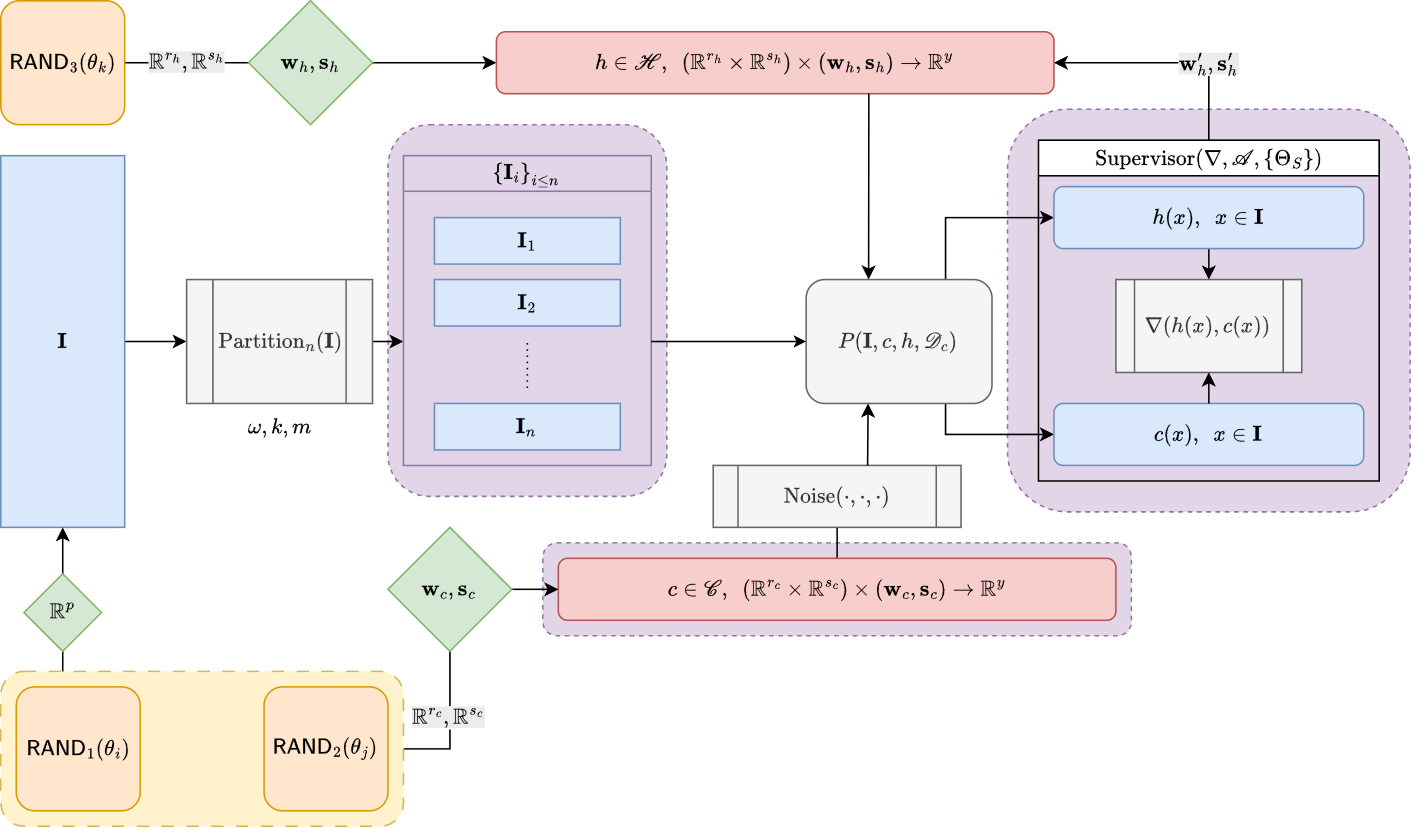
\includegraphics[width=0.65\textwidth]{media/diagram_2.png}
  \caption{\textbf{Diagrammatic view for the ambiance space of the modelling scenario setting, with PAC-learning highlighted focus}. We highlighted (in purple) the main component considered in the formal definition of PAC-learning criteria, minus the bounds on $\epsilon$ and $\delta$, which belongs to the measure.}
  \label{fig:vapnik_scheme_1}
\end{figure}

For VC-style bound, it is partially extended, of which then includes also a description of the hypothesis class, but with a caveat - it depends on the proxy measure of shattering and discrete permutation structure, of which, we can say that it \textit{partially reflects} the hypothesis set in a sense. Additionally, it also takes into account the distribution, as VC-bound type often conjectures on having certain bad distribution in its lower-bound. 

\begin{figure}[htb]
  \centering
  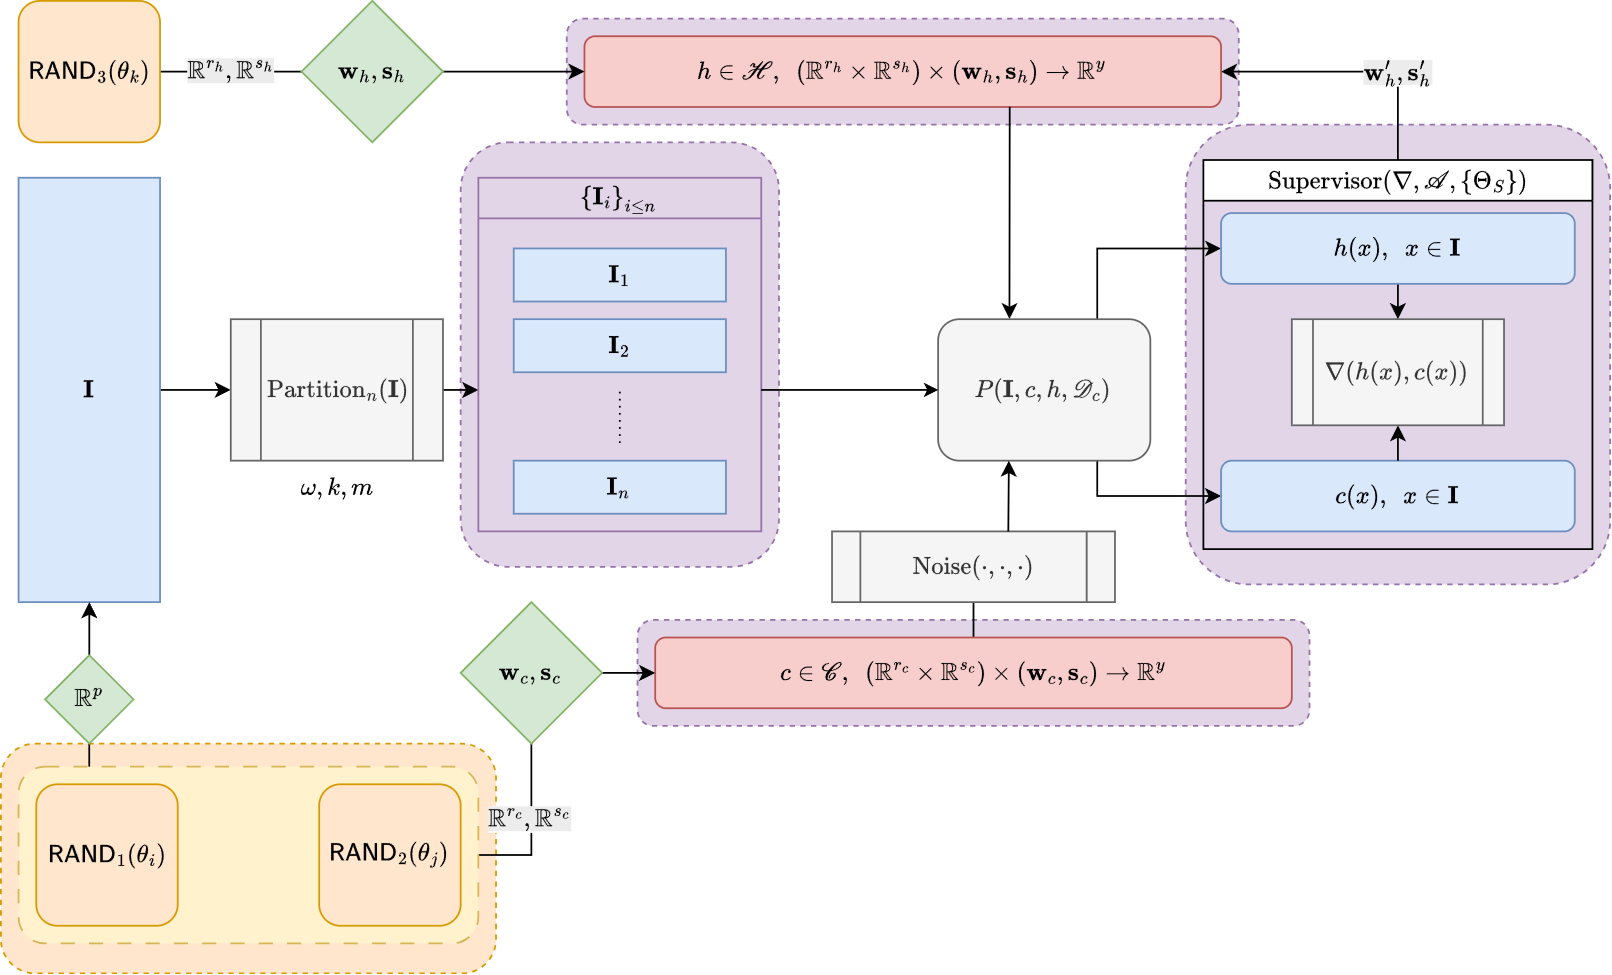
\includegraphics[width=0.65\textwidth]{media/diagram_3.png}
  \caption{\textbf{Diagrammatic view for the ambiance space of the modelling scenario setting, with VC-learning highlighted focus}. We highlighted (in purple) the main component considered in the formal treatment of VC-bound, with the additional (usual) factor of the randomization distribution in the randomizer (in dark orange).}
  \label{fig:vapnik_scheme_2}
\end{figure}

Occam-learning setting works the same as PAC, with a stronger bound emphasis, so we would not include it here, but implicitly define so. Generally, the chain of correspondence which is not directly included in the figures mean that those factors are hidden, either by the assumption of inexpressibility - the inability to know every detail, or certainly of simplifying the bounding methods. 

\subsection{Polynomial space approximation}

Polynomial space is one of those famous example that is often cited of the bias-variance tradeoff. Indeed, it is considered, usually, a very effective and high-volatility construct class. However, what does this mean, is rather implicit. 

Fundamentally, given the univariate case, for a finite sample space $\mathcal{S}^{\lvert n\rvert}$, of fixed range $[a,b]$ correspond to the infimum and maximum of the dataset, $[\min s_{i},\max s_{i}]$ for $s_{i}\in \mathcal{S}^{\lvert n\rvert}$, the problem of polynomial regression is indeed the problem of \textit{soft interpolation}. That is, it basically interpolates based on a constrained response sequence, and where chaotic behaviours can ensue. For our statistical structure to be effective, we will have to use them accordingly. For any model of polynomial regression that want to optimize this specific dataset $\mathcal{S}$, given a free-arbitrary interpolation polynomial $p_{n}(x)$ in univariate space, means fitting to $n$ points specifically such that the polynomial passes each point without any margin of error. This can be done (\cite{McArtneyInterpolation2003}) in either of the parameter basis $\{x^{i}\}^{n}$ up to $n$th degree, of which results in finding the solution for a polynomial 
\begin{equation}
    p_{n}(x) = a_{0} + a_{1} x + a_{2} x^{2} + \dots + a_{n}x^{n} 
\end{equation}
such that $p_{n}(x_{i})=f(x_{i})$, for any arbitrary $f$ of which shape is not known or rather irrelevant of the problem, and for $j=0,1,\dots,n$ (hence there are $n+1$ points). From such, means we require 
\begin{equation}
    p_{n}(x) = a_{0} + a_{1} x_{j} + a_{2} x^{2}_{j} + \dots + a_{n}x^{n}_{j} = f(x_{j}), \quad 0 \leq j \leq n 
\end{equation}
giving a system of $n+1$ linear equation to determine the $n+1$ unknowns $a_{0},a_{1},\dots,a_{n}$. This system of equation has a unique solution, often time, if its \textbf{Vandermonde matrix} $\mathbf{V}$ is nonsingular, or rather, for the determinant of the Vandermonde matrix to be nonzero, \begin{equation}
    \det{\mathbf{V}} = \prod (x_{i}-x_{j}) \ne 0 , \quad 0 \leq j < i \leq n 
\end{equation}
hence giving us the interpolating solution. Hence, we can somewhat guarantee that of the $n+1$ points of which none coincides, then there exists an $n$-th degree polynomial that interpolates to this particular dataset. Usually, polynomial regression uses the same basis for this, hence giving their solution in that respect of the monomial basis. In certain cases, interpolation is basically impossible if our dataset is larger than the number of degree taken, which is typically what is of the polynomial regression case for $n$-basis. This suggests that the number of dataset directly affect the interpolation problem. One result from this is naturally the reduction of the requirement of interpolation, giving us \textit{polynomial regression} - which in such sense is indeed a soft-version of interpolation. Nevertheless, it means we require the system to solve 
\begin{equation}\label{eq:soft_hard_interpolation}
\begin{bmatrix}
1 & x_0 & x_0^2 & \cdots & x_0^n \\
1 & x_1 & x_1^2 & \cdots & x_1^n \\
\vdots & \vdots & \vdots & \ddots & \vdots \\
1 & x_n & x_n^2 & \cdots & x_n^n
\end{bmatrix}
\begin{bmatrix}
a_0 \\
a_1 \\
\vdots \\
a_n
\end{bmatrix}
- 
\begin{bmatrix}
f(x_0) \\
f(x_1) \\
\vdots \\
f(x_n)
\end{bmatrix}
\leq \epsilon
\end{equation}

for a particular $\epsilon > 0$, called the \textit{strength} of the interpolating-with-data parameter. It is trivial to see $\epsilon = 0$ results in the perfect interpolation problem. Note that for this to succeed, the basic intuition is that for $n+1$ points, beyond the constant term, there exists an $n$th degree polynomial with $n+1$ saddle point to wiggle, or rather $n$-degree of freedom of the fundamental monomial basis. 

\begin{figure}[htb]
    \centering
    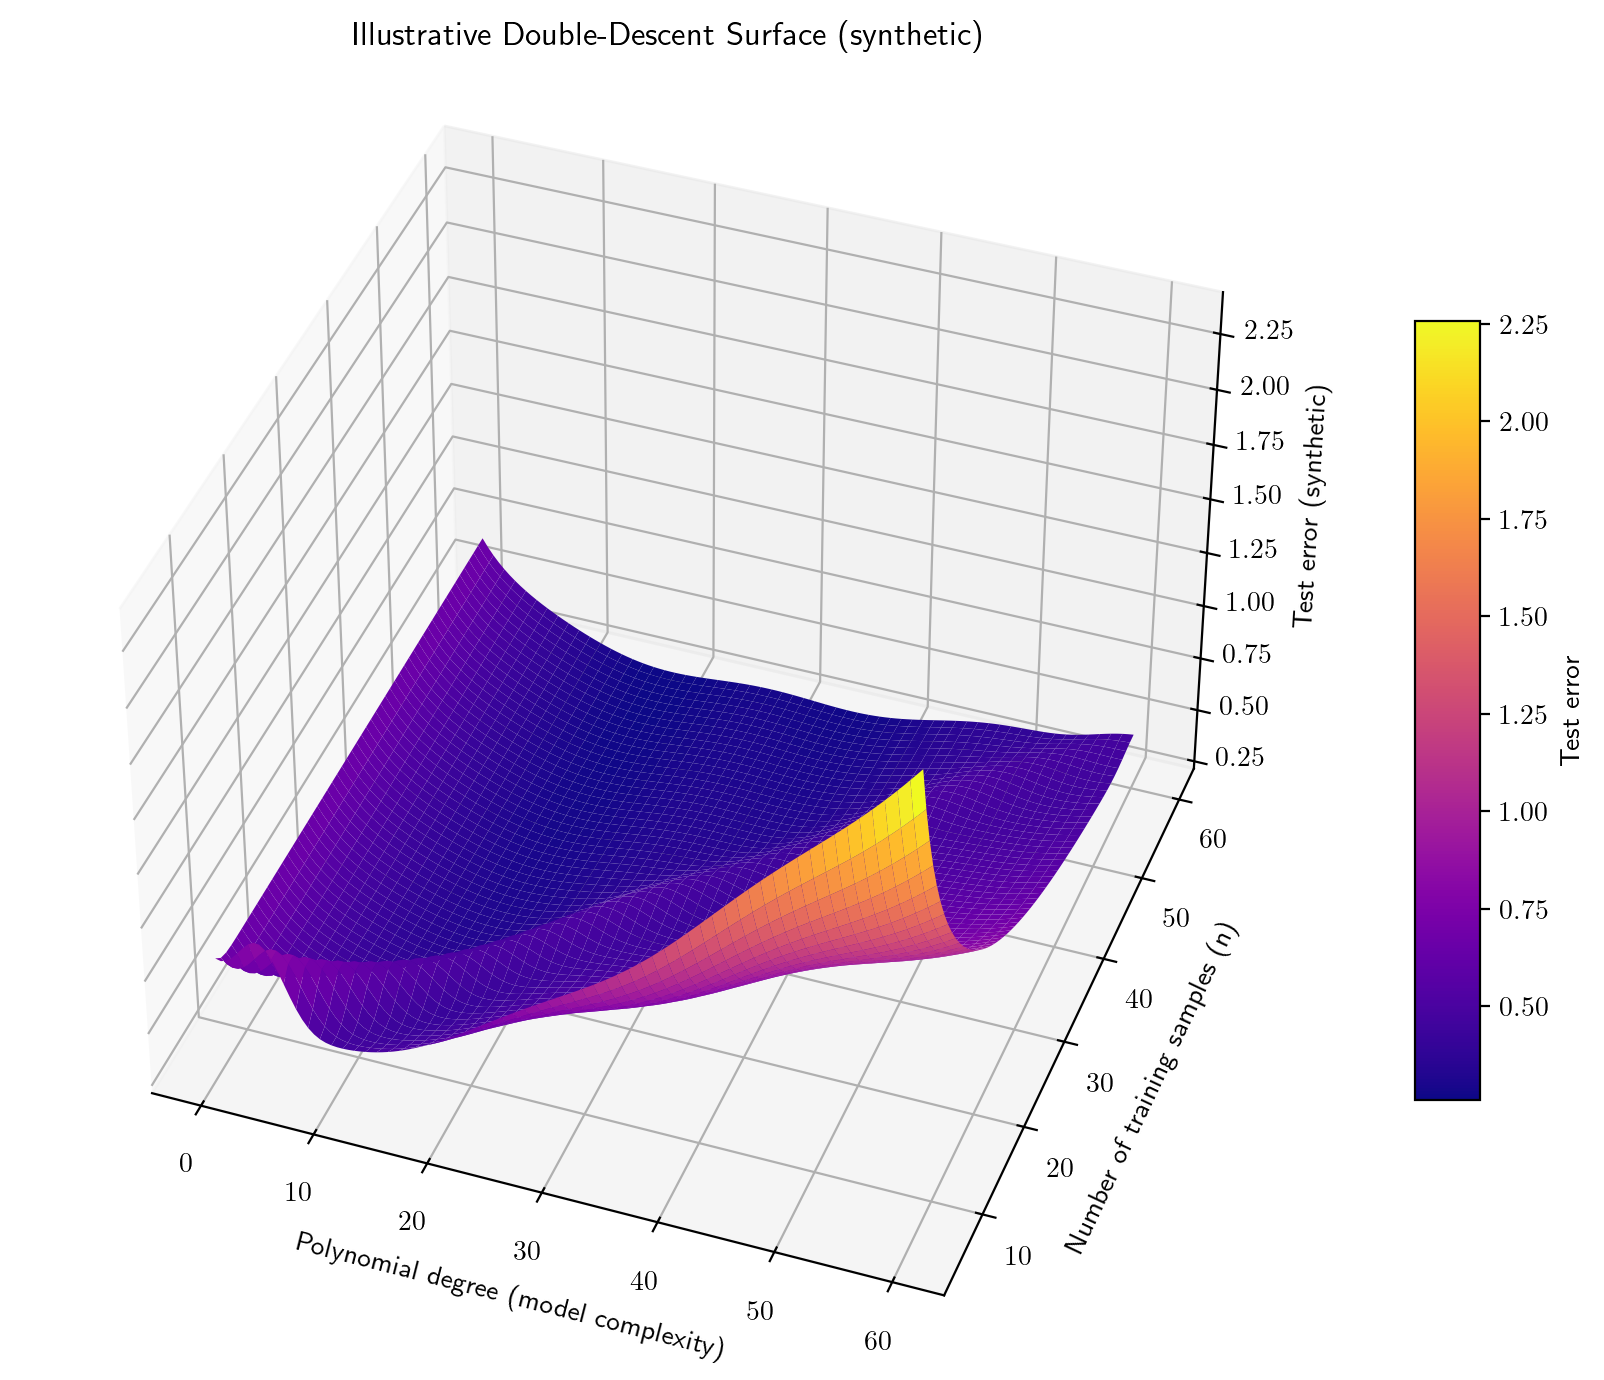
\includegraphics[width=0.55\textwidth]{media/double_descent_synthetic.png}
    \caption{Synthetic double descent curve illustration, with 3 axes of dependency supposed of the parameterization case - the axis of the number of data point in soft interpolation, the saddle points given of the model, and the overall error observed of the model. We did not take into account the relative curve of the test error.}
    \label{fig:descent_synthetic_curve}
\end{figure}

In this particular fundamental space, we can somewhat define the notion of underparameterization and overparameterization in the context of an algorithmic optimization task. This might very well align with the considerable double descent. Hints from this particular polynomial construct means we want to have particular analysis that looks like Figure~\ref{fig:descent_synthetic_curve}, but with some caveat. 

Generally, as for other experiments in this particular paper, we would be entitled to see particular trajectory specifically designed around the point of interpolating match, or $n=m$ of $n$ degree of freedom, technically, and $m$ data points. After this point, there exist two possibility of dynamic - either the model dilutes, in which case result in \textit{double descent}, or the model fluctuate strongly afterward, leading to \textit{bias-variance emergence} again later on. This conclusion however, would have to be analysed within the current framework of the possible interjection to its fluctuation strength. For example, in the monomial basis $\{x^{i}\}^{n}$, any given fluctuation contributes to the entire polynomial. In such case, fluctuation of the other $[0,n-k]$ of arbitrary $k$ and large enough $n$ would be unaccounted for by the scale. Conversely, restrict them to $[1,0]$ range will reveal something about the system, however will destroy particular properties of the prediction, which is not recommended. Nevertheless, we must conduct the test before giving in any reasonable conclusion.

Previously, we said that we did indeed focus on the interpolation problem. Now, assuming we have given the interpolating algorithm $\mathcal{A}$ to approximate the interpolation, what will this look like? First of all, solving this is \textit{very computationally expensive}, because it is a dense, $(n+1)\times(n+1)$ linear system, and even more so if we consider the overparameterized outcome. However, this can be reduced further down if we attempt to solve them using convergence boun, but will be still very expensive. That and incremental soft interpolation is somewhat out of the question since it will be kind of the same. Aside from the insight, we would still have to know what to do. Then there exists two ways - we have some version of this to optimize of simply evaluating by gradient descent optimization, or, we can use somewhat analytical fit for the case of soft interpolation modification. 

A theory on such problem can be obtained of its mechanics, as will be a fairly intuitive way in consideration of the theory of interpolation, as well as the technique of interpolation by itself. For a fixed-range interpolation threshold problem, a hard-encoded interpolation solution requires $n$-degree polynomial, of which has $n+1$ degree of fitness, to fit $n+1$ distinct points. Suppose all points are distinct of the set $S$ which is finite, then this is the case. If we switch to the problem of interpolation but induce a more forgiving bound, there exists a possibility that it induces a relative \textit{density averaging path} for the points, especially if we are considering the case where $p>n$ for $p$ saddle points or degree of fitness, and $n$ the number of point to interpolate. In a more nuanced formulation, we have

\begin{equation}\label{eq:soft_hard_interpolation_role}
\begin{bmatrix}
1 & x_0 & x_0^2 & \cdots & x_0^p \\
1 & x_1 & x_1^2 & \cdots & x_1^p \\
1 & x_2 & x_2^2 & \cdots & x_2^p \\
\vdots & \vdots & \vdots & \ddots & \vdots \\
1 & x_p & x_p^2 & \cdots & x_p^p \\
\vdots & \vdots & \vdots & \ddots & \vdots \\
1 & x_n & x_n^2 & \cdots & x_n^p
\end{bmatrix}_{n\times p}
\begin{bmatrix}
a_0 \\
a_1 \\
a_2 \\
\vdots \\
a_p
\end{bmatrix}
- 
\begin{bmatrix}
f(x_0) \\
f(x_1) \\
f(x_2) \\
f(x_3) \\
\vdots \\
f(x_n)
\end{bmatrix}
\leq \epsilon
\end{equation}
or equivalently, $\mathbf{X}_{n\times p}\mathbf{w}_{n}-\mathbf{Y}_{n}\leq \epsilon$. This essentially is the problem of solving $n$ points approximation, toward using only $p$ saddle points available. If $\epsilon =0$, it is well known that interpolation is impossible. However, if $\epsilon\ne 0$, there are possibilities, depends on the shape of the dataset, that there will exist a data-dependent property or more that indict a particular \textit{density preference} toward those saddle points - or rather, the act of density averaging. Formally, we have the following hypothesis

\begin{hypothesis}
For a polynomial $\{a_{i}x^{i}\}_{n}$ on Vandermonde basis, approximating on the set $\{(x_{k},y_{k})\}_{m}$, then
\begin{enumerate}[topsep=1.5pt,itemsep=1pt]
  \item For $n<m$, we expect the polynomial form factor to be \textit{inherently sparse}, such that for an iterative approximation, for each $p_{i}$ saddle point of the polynomial expansion form, there exists an $\epsilon$-ball $B_{\epsilon}$ for $\epsilon>0$ with at least one data point satisfying $(x_{k},y_{k})\in B_{\epsilon}$. 
  \item For $n=m$, we expect the polynomial to be able to fit all points, up to hard interpolation threshold such that $\hat{R}_{S}\approx 0$. 
  \item For $n>m$, we expect the polynomial form factor to be \textit{locally dense} then turning to \textit{globally dense}, over random ensembles. That is, for every point $(x_{k},y_{k})$ there exists a $\beta$-ball $B_{\beta}$ such that there is at least one saddle point of the polynomial belong to the ball. 
\end{enumerate}
\end{hypothesis}

The shift that will be hypothesized to appear here is expected to be from sparse in the polynomial term sense, out to globally dense with enough model complexity, over an iterative process. One also main point of clarity is, at certain point right now, we haven't discovered the effect of error deviation, yet. For such, I theorized the following. 

\begin{conjecture}[Double descent]
  Double descent happens, for a polynomial class model $h_{n}\in\mathcal{H}_{p}$, is upper bounded to certain error deviation $\epsilon>0$ from the mean only of the generalization (test) dataset verification. 
\end{conjecture}

That is, the disparity between the test and training dataset helps in such regard. If the two dataset is partitioned in the sense that their deviation is practically the same (which can be done using synthetic generation for a control group), then this will amount to not much of it. After all, it will be the consequence of the algorithm and error landscape interpretation used. 

For this, we propose another speculative observation beside such, as to consider adjourned transform of the Vandermonde basis to the Newtonian or similar basis, in which the effects and motion can be easily observed, as least easy. This is because aside from mapping down to $[-1,1]$, normal polynomial on monomial basis gives suboptimal result because of intrinsic high-degree term domination. 

\subsubsection{Stone-Weierstrass theorem}

One of the important aspect of the polynomial class functions is expressed in the form of the Stone-Weierstrass approximation theorem, of which states that every \textbf{continuous} function defined on a closed interval $[a,b]$ can be approximated as closely as desired by a polynomial function $p(x,n)$. The original proof of [Weierstrass, 1885] is done using one type of smooth interpolation, the \textbf{Weierstrass transform}. 

\begin{theorem}[Weierstrass Approximation Theorem]
    Let $f\in C([a,b],\mathbb{R})$ of continuously differentiable space. Then there is a sequence of polynomial $p_n (x)$ that converges uniformly to $f(x)$ on $[a,b]$.     
\end{theorem}

Using function algebra, we can generalize such approximation notion to a wider structure, of subalgebras on Hausdorff space. 

\begin{theorem}[Stone-Weierstrass Theorem (real version)]
  Let $S$ be a locally compact Hausdorff space. Let $A$ be the subset of bounded continuous real functions on $X$, or of subalgebras $\mathcal{C}(X,\mathbb{R})$ which contains a non-zero constant function, then $A$ is uniformly dense in $\mathcal{C}(X,\mathbb{R})$ if and only if it separates points. 
\end{theorem}

This will become more relevant later on in the analysis. 

\clearpage

\subsection{Linear correspondence classes}

Linear-linear scenario learning is one particularly well-studied case of representing double descent or not, usually through simplicity in analysis (of the similar ease of proof compared to binary classification). Models in this setting can be said to share the same \textit{parameter space} with no additional structure or scaling mask (like in monomial basis). The model that is representative of this preliminary observation is from \cite{lafon_understanding_2024}, specifically, linear regression (function approximation) with Gaussian noise, and of univariate case. Consider the family class $(\mathcal{H}_p)_{p\in\llbracket1,d\rrbracket}$ of linear functions $h:\R^d\mapsto \R$ where exactly $p$ components are non-zero ($1\leq p\leq d$), we have the following model.

\begin{definition}
For $p \in \llbracket1,d\rrbracket$, $\mathcal{H}_p$ is the set of functions $h:\R^d\mapsto \R$ of the form:
$$
h(u)=u^Tw,\quad \text{for }u \in \R^d
$$
With $w \in \R^d$ having exactly $p$ non-zero elements. The complexity here itself can be interpreted as the effective random initialization, trimming down data of hidden details instead - this is indicated by the amount of information it observes given $d$ dimension, and $p$-hypothesis dimension. \footnote{According to the \textit{manifold hypothesis}, there are chances where the actual concept can be interpreted and mimicked by seeing that it lies on a lower-dimension manifold inside its actual expressive dimensional space. }
\end{definition}
Using such model, they consider the setting of minimizing the customized mean square loss, 
\begin{equation}
\label{eq:linear_gaussian_erm}
\min_{w\in \R^d} \frac{1}{2}\norm{\bm{X} w - \bm{Y}}^2 \to \min_{w\in \R^p} \frac{1}{2}\norm{\bm{\Xp} w - y}^2
\end{equation}
of the sub-problem on $p$ cardinality, where again $p$ is the dimensionality or independent degree of freedom. This results in the following theorem that 'mimic' double descent on this linear regression model.
\begin{theorem}[Double descent on linear regression]
\label{thm:double_descent_lr}
Let $(x, \epsilon)\in \R^d\times\R$ independent random variables with $x \sim \mathcal{N}(0,I)$  and $\epsilon \sim \mathcal{N}(0,\sigma^2)$, and $w \in \R^d$. we assume that the response variable $y$ is defined as $y=x^Tw +\sigma \epsilon$. Let $(p,q) \in \llbracket 1, d\rrbracket^2$ such that $p+q=d$, $\bm{\Xp}$ the randomly selected $p$ columns sub-matrix of X. Defining $\hat w:=\phi_p(\p{\hat w},\q{\hat w})$ with $\p{\hat w}=\bm{\Xp}^+y$ and $\q{\hat w} = 0$.\\
The risk of the predictor associated to $\hat w$ is:
\begin{equation}
    \E[(y-x^T\hat w)^2] = 
\begin{cases}
(\norm{\wq}^2+\sigma^2)(1+\frac{p}{n-p-1}) &\quad\text{if } p\leq  n-2\\
+\infty &\quad\text{if }n-1 \leq p\leq  n+1\\
\norm{\wp}^2(1-\frac{n}{p}) +  (\norm{\wq}^2+\sigma^2)(1+\frac{n}{p-n-1}) &\quad\text{if }p\geq n+2\end{cases}
\end{equation}
The point $p=n$ is representative of the interpolation threshold from underparameterization to overparameterization. 
\end{theorem}

As said, this theorem is designed to mimic the double descent behaviour on the range of linear regression with Gaussian noise. While there exists a proof for this particular theorem, to rule out possible falsification, experiment to verify the claim of this particular result will have to be conducted. 

We present two parts - first are those fundamentals predicted by the theorem, and second are verifications of the theorem with our own version of testing. The first experimental setting is then conducted with fixed $d$, varying $p$ for each varying $n$ samples. Since this is a least square result, preliminary run is conducted using one-shot error-risk measure on least square closed-form approximation. Note that $p\leq d$, hence we are regarding the domain of the term underparameterized and equal parameterization setting. The result is presented in Figure~\ref{fig:theorem_double_descent_fig}

\begin{figure}[htb]
    \centering
    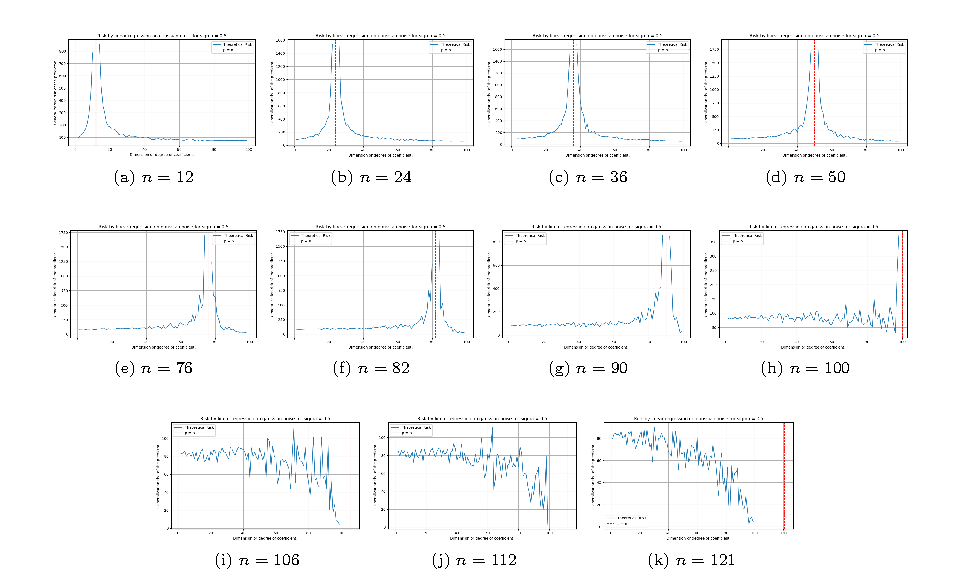
\includegraphics[width=0.8\textwidth]{pdf/theorem_1.pdf}
    \caption{Theorem~\ref{thm:double_descent_lr} behaviours on randomized setting. For this model, we have $d=100$, $\sigma = 0.5$, and variational $n$. Full test cases are for $p=[1,100]$, $n=\{12,24,36,50,76,82,90,100,106,112,121\}$ accordingly. The test function of the concept itself is the same linear model, but with different input only.}
    \label{fig:theorem_double_descent_fig}
\end{figure}

As we see from this particular experimental result, the theorem predicted a loose, left-peak absent, double descent curve estimation for a variety of test case with more and more samples in increment. There exist some fundamental conclusion that we have about the shift of the interpolation threshold upon to $p=n$, which is reflected in the piecewise prediction. However, this pattern breaks down for $n$ higher than specific constant, for this case, starting from $n\approx 100$ to beyond. From here, at least from testing scenario, the test indicates that predictions suggest a breakdown of the double descent estimation. Beyond this, a simple semi-chaotic convergences is observed, from $n=106,112, 121$. 

Interestingly, verifying this notion of easy enough to simplify it into what the statement holds under particular notion. Namely, as we find out, the above double-descent replicating formula can actually be realized by the parameter-wised error, comparing the parameter between the least-square solution and the actual concept. The formula for this is expressed by the exposed MSE on parameter function, for $\beta_{p,k}$ the coefficient value estimated for the $k$-th selected feature when the model is restricted for randomization of $p$ features, 
\begin{equation}
\mathrm{MSE}_{\mathrm{param}}=\left\lvert \hat w - w \right\rvert _{2}^{2}=
\sum_{j=1}^{d}
\left(
  \hat w_{j} - w_{j}
\right)^{2}
\end{equation}
where $\hat w_{j}$ is chosen such that it is equal $0$ for $j \notin S$, otherwise $\beta_{p,k}$ for \(S=\{i_1,\dots,i_p\}\) is the set of selected feature indices. Nevertheless, it is then found dubious why this is true, as for the original statement of \cite{lafon_understanding_2024} indicates correlation to the prediction error of the result, $x^{\top}\hat{w}$ instead. The result of evaluating $\mathrm{MSE}_{\mathrm{param}}$ is presented in Figure~\ref{fig:theorem_double_descent_fig2}.

\begin{figure}[htb]
    \centering
    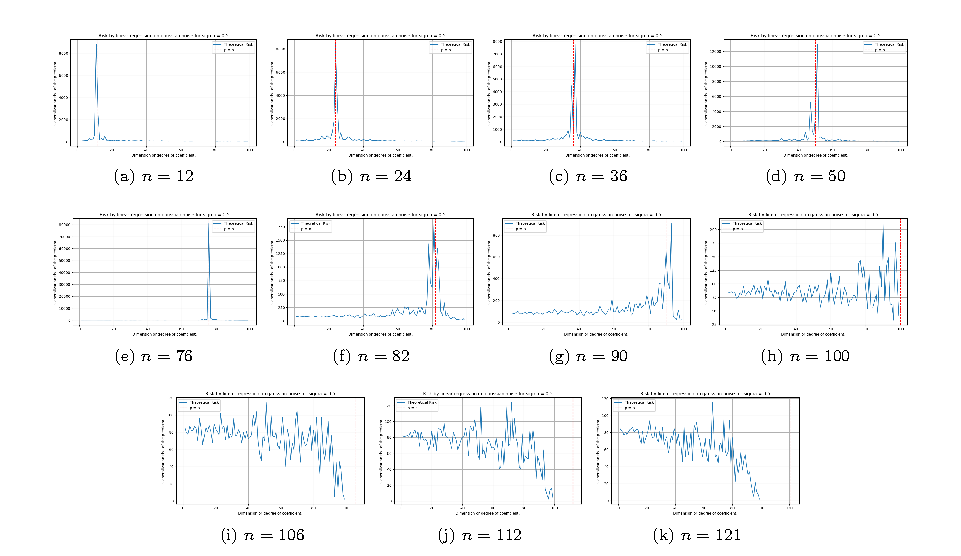
\includegraphics[width=0.8\textwidth]{pdf/theorem_2.pdf}
    \caption{Contrary to Theorem~\ref{thm:double_descent_lr}, this is the behaviours on randomized setting for standard parameter-wised mean square error measure (MSE-on-parameter). For this model, we have $d=100$, $\sigma = 0.5$, and variational $n$. Full test cases are for $p=[1,100]$, $n=\{12,24,36,50,76,82,90,100,106,112,121\}$ accordingly. The test function of the concept itself is the same linear model, but with different input only.}
    \label{fig:theorem_double_descent_fig2}
\end{figure}

If, however, we turn our attention to the statement itself, of which refers to the prediction error $\mathrm{MSE}_{\mathrm{pred}}$\footnote{The standard formulation in question is \begin{equation}
\mathrm{MSE}_{\mathrm{pred}}
=
\frac{1}{n}
\left\lVert
  y - X_{p}\,\hat\beta
\right\rVert_{2}^{2}
=
\frac{1}{n}
\sum_{i=1}^{n}
\left(
  y^{(i)} - x_{p}^{(i)\,T}\,\hat\beta
\right)^{2}
\end{equation}} on $h$ and $c$ accordingly, a strong case of this happens to be not following the pattern indicted by the theorem. Rather than being the interpolation point of return, $p=n$ is now the convergence point of the prediction error instead. Test result is shown in Figure~\ref{fig:theorem_double_descent_fig3}.

\begin{figure}[htb]
    \centering
    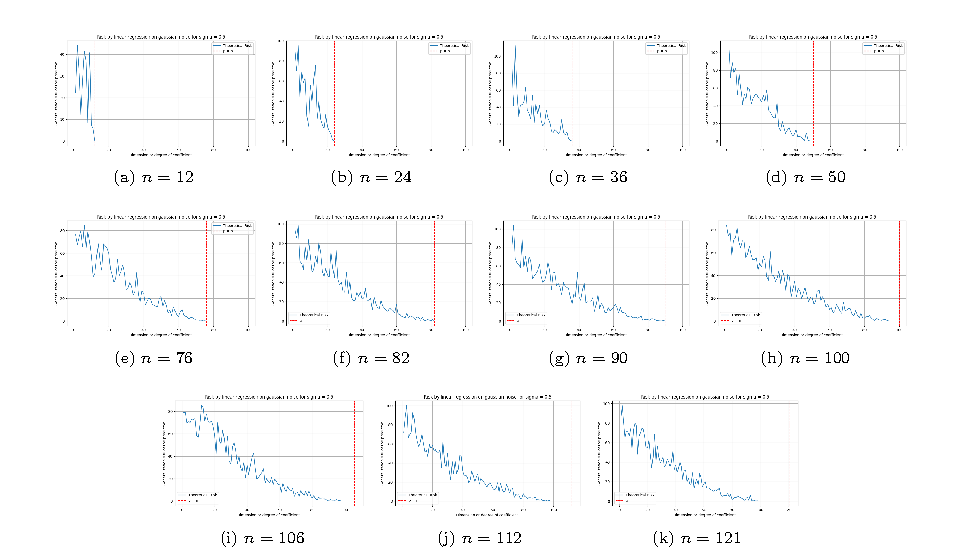
\includegraphics[width=0.8\textwidth]{pdf/theorem_3.pdf}
    \caption{Contrary to Theorem~\ref{thm:double_descent_lr} and both figure~\ref{fig:theorem_double_descent_fig2}, this is the behaviours on randomized setting for standard parameter-wised mean square error measure (MSE-on-prediction). Especially, we do not see double descent pattern in this setting, as it is. For this model, we have $d=100$, $\sigma = 0.5$, and variational $n$. Full test cases are for $p=[1,100]$, $n=\{12,24,36,50,76,82,90,100,106,112,121\}$ accordingly. The test function of the concept itself is the same linear model, but with different input only.}
    \label{fig:theorem_double_descent_fig3}
\end{figure}
\begin{figure}[htb]
  \centering
  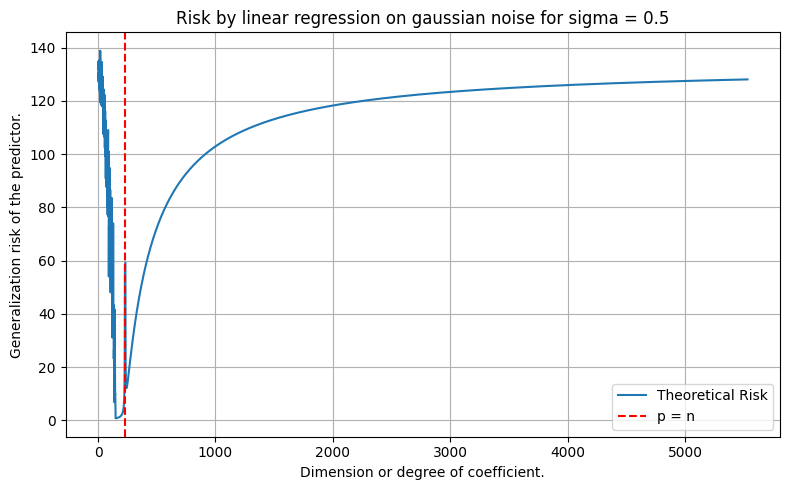
\includegraphics[width=0.6\textwidth]{media/dimensional_descent.png}
  \caption{Similar experiment according to setting and result of Theorem~\ref{eq:linear_gaussian_erm}, where $p$ is in the range [1,5523]. Here, we can see small double descent modelled exactly at the interpolation threshold, while the later region exhibit similar phenomenon as bias-variance tradeoff.}
  \label{fig:contrarian}
\end{figure}
Thence, the theorem gives us two things - the interpolation point, in this setting, refers to the parameter error for their double descent behaviour. However, on the prediction results' error measure, the interpolation point correlates to the point where the defined generalization risk in such case equals zero. These patterns hold up to certain point. However, the test case is only up to $d=p$. An unexplored test case for $p>d$ indicate the surprising fact according still, to the theorem: the generalization risk takes double descent as a region with disturbance in the middle, but bias-variance appears afterward. This is illustrated in Figure~\ref{fig:contrarian}, where the same theorem is applied but in the domain which is usually called as \textit{overparameterized region}. 

\subsubsection{Verification}

To verify the theorem itself, we test it with a standard setting without the theorem results. This is reflected in Figure~\ref{fig:theorem_double_descent_fig}. The result is somewhat consistent with the theorem and its latter parameter error and prediction error results, however, this time, it correlates exactly as the prediction error instead. Additionally, peculiarity occurs in the non-double descent region, with much less volatility than in the prediction of the theorem. 

\RestyleAlgo{ruled}
\SetKwComment{Comment}{}{}
\begin{algorithm}[htb]
    \caption{Linear regression with Gaussian white noise, full control.}
    \KwData{$n,p,d,\sigma,r$, fixed range $[a,b]$, $u\in [0,1]$}
    \KwResult{Threefold error measure - MSE on parameters $p,d$, MSE on prediction $Y',Y$, and theoretical risks measure by prescription.}
    \Begin
    {
    $\mathrm{Randomizer}(\cdot)\gets\mathrm{PCG64}(n\leq 100)$\Comment*[r]{Randomizing pseudo-random engine}
    $\sigma\gets 0.5$, $d\gets 150$\Comment*[r]{Common presetting for parameters}
    $nl\gets\{12,24,36,50,76,82,90,100,106,112,121,150,231,250,256,280\}$\Comment*[r]{Common full-list $n$ count of datapoints}
    $p\gets 150$\Comment*[r]{Underparameterization to equal}
    $\mathbf{p}\gets \mathrm{range}(1,p)$\; $[a,b]\gets [-100,100]$\;
    $w_{c}\sim \mathrm{PCG64}.\mathrm{Uniform}([1,d],150)$\; $b_{c}\sim \mathrm{PCG64}.\mathrm{Uniform}([1,10])$\;
    $w_{p}\sim \mathrm{PCG64}.\mathrm{Uniform}([1,p],p)$\; $b_{p}\sim \mathrm{PCG64}.\mathrm{Uniform}([1,10])$\;
    $X\sim\mathrm{PCG64}.\mathrm{Uniform}(\mathrm{range}\gets[a,b],\mathrm{size}\gets[n,d])$\Comment*[r]{$n$ samples of $d$ dimensions.}
    $\mathrm{concept}(\cdot,\cdot,\cdot)\gets (d,w_{c},b_{c})$\;
    $Y \gets \mathrm{concept}(X, w_{c},b_{c})$\;
    $\sigma_{\mathrm{scaled}} \gets \sigma \cdot \mathbb{E}\left[\lvert Y\rvert\right]$\;
    $Y \gets Y + \mathrm{PCG64}.…\mathrm{Normal}\left(\mu\gets 0,\;\sigma\gets \sigma_{\mathrm{scaled}},\;\mathrm{size}\gets\lvert Y\rvert\right)$ \Comment*[r]{Noisy featuring}

    \For{$n\in nl$}{
        $w_{p}^{*}\gets\mathrm{PCG64}.\mathrm{Permutation}(d,p)$\;
        \For{$i\gets 1$ \KwTo $\lvert w_{p}\rvert$}{
            \If{$i\neq w^{*}_{p}$}{
                $w_{p}[i]\gets 0$, fixed zero point. 
            }
        }
        $\mathrm{model}(\cdot,\cdot,\cdot)\gets (d,w_{p},b_{p})$\;
        $Y\gets \mathrm{model}(X,w_{p},b_{p})$\;
        $\mathrm{approx}\gets \mathrm{LeastSquare}(\mathrm{model},Y',X,Y)$, fixed $w_{p}$.
    }
    $\mathrm{MSE}_{\mathrm{param}}(\cdot,\cdot,\cdot)\gets \mathrm{MSE}(Y,\{\mathrm{approx}\},\mathrm{model})$\;
    $\mathrm{MSE}_{\mathrm{pred}}(\cdot,\cdot)=\mathrm{MSE}(Y,Y')$
    $\hat{R}_{\mathrm{Thm}}=\mathrm{TR}(w_{c},\sigma,p,d,n)$\;
    }
    \Return{$\mathrm{MSE}_{\mathrm{param}}$, $\mathrm{MSE}_{\mathrm{pred}}$,$\hat{R}_{\mathrm{Thm}}$}
    \label{algo:algo_reg_lin_1}
\end{algorithm}

We use the Algorithm~\ref{algo:algo_reg_lin_1} for verification, including three modes of error measure, which will then be calculated accordingly. For gradient descent, we refer to another experiment. For such algorithm, we notice that the operational space of the model is $\mathbb{R}^{n}\to \mathbb{R}$. The masking of parameters then is not well-received, since the output space is far more skewed - single dimension resultant with no scaling difference because the model in question is supposed to be linear. Regarding such, it makes sense to realize that the model itself can still attain relatively stable error, because its feature compounds on the scaling parameters

To test the stability of the model, we run for a stable section of the permutations done on $p$. The result is outlined in \ref{fig:theorem_double_descent_fig}. Interestingly, while the interpolation threshold theorized being $p=n$ does not hold, the pattern of double descent without head descent still fundamentally exists, albeit in a much more constrained region, as can see from $n=12$ to $n=150$. The pattern from then onward follows a reduced trend, without the chaotic behaviours seen. The result is shown in Figure~\ref{fig:theorem_double_descent_fig4}.

\begin{figure}[htb]
    \centering
    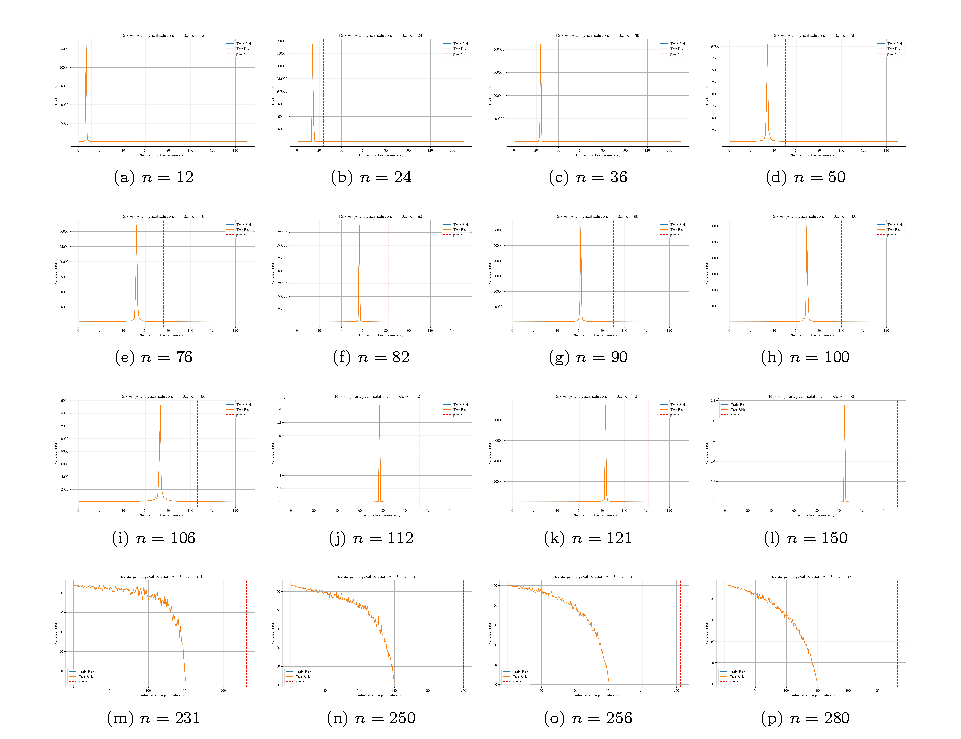
\includegraphics[width=0.8\textwidth]{pdf/theorem_4_verify.pdf}
    \caption{Risk curves for varying sample size $n$ (dimension $d=100$, noise $\sigma=0.5$). Double descent is determined in similar sequence, even though the interpolation theoretical $p=n$ is actually shifted over to the right from the actual interpolation observables, in parameterization. Afterward, correlation fails, and the theoretical $p$ is ineffective, similar to previous theorem-based test run. Sample set size range is $n\in\{12,24,36,50,76,82,90,100,106,112,121,150,231,250,256,280\}$. One additional remark is that the error landscape is relatively thin in either side, making it abnormal in comparison to actual bias-variance curvature.}
    \label{fig:theorem_double_descent_fig4}
\end{figure}

\subsubsection{Remark}

At least from this experiment, overall, results gathered using Theorem~\ref{thm:double_descent_lr} and variations of it suggests inconsistent results. The supposed interpolation threshold has different interpretation and indication in different scenario, including both parameter-wise error and prediction-only error measure. Furthermore, verification also shows inconsistency with the interpolation threshold, albeit given the fact that the margin of error from the highest peak to the interpolation point is consistent up to certain $n$. Breakdown of the result from theorem, as well as double descent behaviour starts with high $n$ counts, as well as interesting outlook of bias-variance reappearance for $p\sim 5000$, far more than what is tested in normal testing cases. Such result suggests further experiments to validate the observations, as well as statistical analysis of the entire system. 

Specifically, the interpretation of the result is not perfect. Under such setting, then for the concept of the same class, so $d=150$, any concept of $p>d$ would result in the metric taking zero value of the `truncated region' where $d$ is literally flat on the $d+1$ onward space. Hence, the error being added on top of such error measure is the component distance of $p$ to the flat sub $p-d$ space itself - which explains the curve going upward, as more and more risks are configured. Nevertheless, the amount of data provided, at least in terms of this model, does indeed have non-trivial effect on the model itself, and the least square solution of best fit which gives the potential minimal, hence the empirical best. Considering the results, we can see regions where the theorem `breaks' of its bias-variance pattern. Further experiment to verify such claim and reconfiguration is needed. Worryingly, in this particular case, there exists no saddle point that was theorized by bias-variance tradeoff, which must then be explained accordingly. Furthermore, we also notice the troublesome fact that this particular pattern works on \textit{same operational space} models, that is, linear models approximating linear models. This setting is fairly limited, and would not generalize well. However, we also do not know what kind of measure to take in such case. Conflicting notions and reports aid into the confusion of such topic more than can be normally observed, and the anomalous behaviours in some researches (for example, in \cite{shi2024homophilymodulatesdoubledescent}, we received that in GNN, there exists no trace of double descent) makes it even harder. As such, both the status of bias-variance being false, albeit in a given range only, and double descent in masking certain behaviours of the modelling process, have taken a mysterious stance in the modern machine learning community.

While discovering the double descent phenomena, it also exposes theoretical concepts that are not organized or formalized, portions of the theory and empirical observations that are within conflict of each others, issues with definitions, theorems, and interpretation of them. Those problems would then ultimately hinder further research in such direction, as well as broader theoretical requirement of the theory of machine learning, and specifically to a larger and more complex system of deep learning. 

\subsection{Support Vector Machine}

Support vector machine, first formally originated from \cite{Vapnik1999-VAPTNO}, is a model inherently, specifically defined for pattern recognition task, and binary classification via an \textit{optimal separating hyperplane}. There are two variants for SVM, namely, for linear and nonlinear hyperplane. 

The SV machine implements the following two precursor ideas: It maps the input vectors $x$, supposed of the setting, into a high-dimensional feature space $Z$ through some nonlinear mapping, chosen a priori. In this space, an optimal separating hyperplane is constructed. By statistical learning theory, Vapnik restricted the function class (as for infinite hypothesis it is impossible to learn) to the class of hyperplanes by 
\begin{equation}
    \langle \mathbf{w}\cdot \mathbf{x} \rangle + b = 0 ; \quad \mathbf{w}\in \mathbb{R}^{n} , b\in \mathbb{R}
\end{equation}
which $\mathbf{w}$ is the controlling weight, $\mathbf{x}$ is the input space to the space of all binary $\{-1,+1\}$ category. Hence, this basically divide the input space into two: one part containing vectors of the class $-1$ and the others being $+1$. If there exists such a thing, then it is said to be \textit{linearly separable}. To find the class of a particular vector $\mathbf{x}$, we use the following decision function 
\begin{equation}
    f(\mathbf{x}) = \mathrm{sgn}[\langle \mathbf{w}\cdot \mathbf{x}\rangle+ b]
\end{equation}
This is called the \textbf{hyperplane classifier} class. As can be understood simply from such, there exists many hyperplanes that can correctly classifies the classes. It has been then shown that the hyperplane that guarantees the best generalization problem performances is the one with the maximal margin of separation between two classes (\cite{Cristianini2000AnIT}). The above form of finding final classification can then be presented in dual form, which then depends only on dot products between vectors, as 
\begin{equation}
    f(\mathbf{x}) = \mathrm{sgn}\left(\sum^{\ell}_{i=1} y_{i}\alpha_{i} \langle \mathbf{x}\cdot \mathbf{x}_{i} \rangle+ b\right)
\end{equation} where $\alpha_{i}\in \mathbb{R}$ is a real-valued variable that can be viewed as a \textit{measure} of how much informational value $\mathbf{x}_{i}$ has (for $x_{i}$ the support vectors we get from training)\footnote{The \textit{support vector} of a particular hyperplane $\mathbf{y}$ is the collections of all points that lies closest to the hyperplane, which is specified as condition for maximization on both side of maximal margin vector machine.}

The second idea is of the \textit{kernel method}. This particular method, useful and well-known of the time SVM was created, gain a more prominent position among other techniques, including neural network. Specifically, this method is characterized by the mapping of the input vectors into a richer (usually high-dimensional) feature space where they satisfy \textit{linear separable} criteria. This prompted the possibility to solve nonlinear problem through such mapping, and indeed yields a nonlinear decision surface in the input space, which is linear in the feature space. A \textbf{kernel} (function) is then a function $k(\mathbf{x},\mathbf{y})$ that given two vectors in input space, return the dot product of their images in feature space such that $k(\mathbf{x},\mathbf{y})=\langle \phi(x), \phi(y) \rangle$ for the nonlinear mapping $\phi$. The general form of SVM is then 
\begin{equation}
    f(\mathbf{x}) = \mathrm{sgn} \left(\sum^{\ell}_{i=1} y_{i}\alpha_{i}k\langle \mathbf{x}\cdot \mathbf{x}_{i} \rangle\right)
\end{equation}
for any particular final categorization. One of the major problem for analysing SVM, is in the properties of it potentially having infinitely many parameters, depends on the size of the dataset. This makes the curve of both bias-variance and double descent not applicable in such regard - infinitely many parameter complexity, yet still finite complexity class. 

From such observation, it would seem imperative that the notion of complexity based solely on the parameter counts of certain model construction is ill-equipped for certain flavours of machine learning model, in this case support vector machine (in the same type is the Gaussian Mixture Model). No double descent has been observed by empirical reports record per the author's knowledge. 

\begin{setting}[Support vector machine]
    We formulate the support vector machine scenario as followed. Let the hypothesis be the class of all $d-1$-dimensional hyperplane opr affine subspace of $d$-dimensional space equipped with kernel, support vectors, and a binary decision rule $\sign{x}\to \{0,1\}$ accordingly. Let the concept $c\in \mathcal{C}$ be the class of all binary categorization that either linearly separable or not. Assume a generalized kernel, $h$ holds no knowledge of $c$ aside from binary separation criteria inherent in its design. Consider the set of observations $\mathbb{O}$ of $h$. Then, it will be controlled of $\mathbb{O}=(\mathbb{U},\mathbb{I})$ where $\mathbb{U}$ is the \textbf{input space} for $k$ points, and $\mathbb{I}\subseteq \{0,1\}^{k}$ is the inferred space of such points. Assume such observations are formed of the distribution $\mathcal{D}^{k}$ on all points. Consider a random $d$-dimensional noise (similar to 1-step random walk) $\mathcal{N}(\cdot)$ or normal distribution $\mathcal{N}(\sigma, \mu)$. The learning process then continues as binary classification for either minimization, and accordingly structural minimization. 
\end{setting}

The complexity in question that would have to be considered and calculated is the support vectors, or rather, the margin point. Though this effectively means that it does not take all data to form the margin, it still means that there then can exist infinite `counting complexity' with respect to the parameter counts. Thereby, we would need another measure of complexity than just as parameters specific to the hypothesis. In fact, the construction of the hypothesis must also consider this aspect itself as a class. 

We tested preliminary SVM with dimension of the feature $p$ in range $[1,80]$, linear kernel, data points increase of the sequence $\{5, 10, 20, 30, 40 , 50, 60, 70 , 80, 100, 120, 140, 150, 160, 170\}$, noise $\sigma = 0.1$, and with distributions almost all being standard normal distribution. Train-test variation is configured with partition scale $0.2$ with random shuffling. Preliminary experiment unfortunately does not give any indication of particularly double descent, and is rather very chaotic. Let us illustrate it. The first case, for $n=20$, normalized, $p=[1,30]$, $\sigma =0.5$, and standard no regularization gives the result in Figure~\ref{fig:test_svm_com_ideal}.

\begin{figure}[htb]
  \centering
  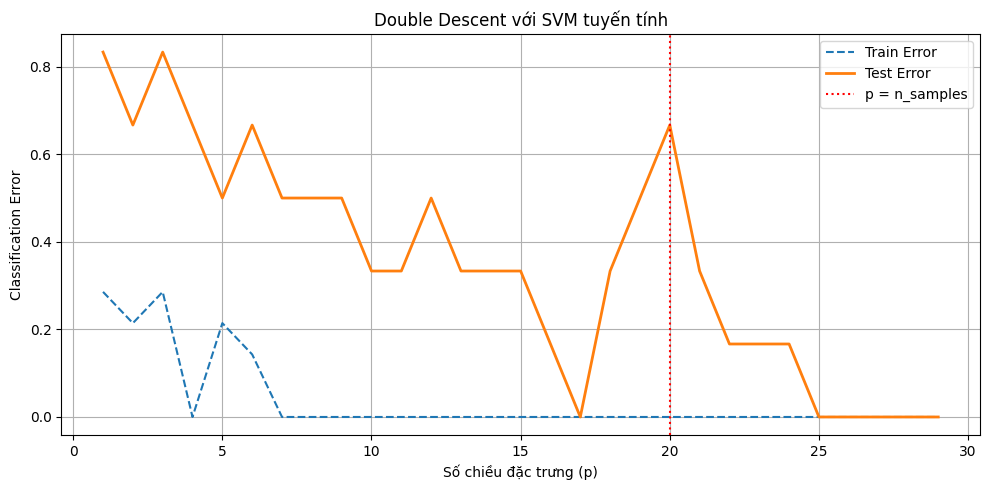
\includegraphics[width=0.5\textwidth]{test_case_ideal_svm.png}
  \caption{\textbf{Experiment on support vector machine on parameterized double descent identification}. The pattern appears marginally on the result graph, with a correct case of interpolation prediction for $p=n$.}
  \label{fig:test_svm_com_ideal}
\end{figure}
However, when we turn our attention to a wider experimental analysis, we gain the following results in Figure~\ref{fig:risk_all_grid_svm}, which is very chaotic. Further experiment is required to validate hypothesis about both, in certain cases, manifold hypothesis's contribution and double descent. 

\clearpage

\section{Experimental instruction}
This part is reserved for experimental testing procedures and so forth. Thereby, it will not be in the instruction set, or in the official paper. More like in a supplementary resource. As its name implies, 

\clearpage

\section{A novel theory proposal}

Motivated by earlier analysis and observations, it is apparent that the analysis is entangled, with various situations, interpretations, setting and assumptions together, and with a non-unified structure of models in question. The system in which the model is considered and analyzed is also ineffective when considering larger structures or more `realistic' consideration aside from very simplified, strong system itself. There are a lot of ambiguities around what is considered and what is not, even with probabilistic nature and the deterministic aspect. Terms like \textbf{latent spaces} and many do not capture the entire dynamic or meaning of the system. It is then we introduce our novel analytical framework, namely the \textbf{Unified Unitary Construct} framework. It is however, can be said otherwise that the learning theory is rather not so novel, but approaching the problem is a more distinct way of the already existing framework. 

\subsection{Principle}

We are motivated from earlier analysis, further experimental results, and arguably practical observations of empirical-based architectures that we find interesting. Oddly enough, the idea is encouraged of the observation that \textit{deep neural network} organising architecture might be more general than it is, particularly in the sense of mathematical modelling and structural implicit approximation, as well as factors like scalability, generality, and else. Furthermore, one of the purpose of this novel theory is also to redefine the entire learning space to, at least if not entirely original, might as well fall into the category of a reformulation of theoretical framework and not partaking the role of replacing it. 

As such, we need some principles to get started the analysis. What can those be that guarantee the success of a particular reformulation at first? For starter, we indict on the requirement of developing a general framework of neural network-like organisation for our models, both in the interpretation of the learning objective, and the structure of the hypothesis learner. Secondly, we have to define learning as a barebone process, of which then we will have to justify \textit{probabilistic nature} of it and the degree in which that is true. Thereby, we will then also have to reconsider the learning problem, under what scope of the problem and the classes of learning that is there to be achieved, the encoding space and what it is meant to, and the criteria of guaranteeing such learning to be probable. For now, those are enough, but the development that come afterward will justify it instead of the principle. 
Nevertheless, we can see the principle here - we want to redefine learning process in an organized manner, with minimal messiness from considering all factors together, and normalize the interpretation of \textit{unit-wise} architecture that neural network uses up to more. 

\subsection{Planning}

Then, what is the plan? The goal is to \textit{systematically introduce} the concept and the novel theory. Hence, we will separate it into discrete small step size parts. First, we need to conform the setting with a new template. This mean the following order is needed. 
\begin{enumerate}[leftmargin=1cm,itemsep=2pt,topsep=2pt]
  \item Introduce and define the formalism of an \textit{ambiance space} and an \textit{encoding space}. Those two will come in together to form the majority of $S$ as per system dynamic notation. 
  \item In the \textit{collection} $S$ should we extend it further, there always exists the object $h$, belonging to certain configuration class $\mathcal{H}$. We need to define this particular object, and its interaction to the collection itself. Which means, the ambiance space and encoding space. How do we bring up the \textit{representation concept} here altogether? 
  \item To start the mechanics, we need the \textit{mechanical space} $M$ to be defined. What can be it? What connects and form the structural description that $S$ make with the ambiance space, encoding, representation, subject dynamics, and else? 
  \item Now, come to the \textit{operational process}. For this, let's assume we have two different systems, in accordances, $S_{1}$ and $S_{2}$, each of which houses $h$, and $c$ respectively. How do they communicate? How, should it be done, can the operational space indict particular objective, or requirement, such that $h$ is evaluated, and $c$ is evaluated? What is hidden of $h$, and what is hidden of $c$? 
  \item Then, finally, bounds, theorems, analytical results, algorithmic consideration and conjectures that fit, into this description. 
\end{enumerate}
From the scope of it, it might seem not too practical to call as novel. But as far as we are considered, there should be something to take account on, and we need to do them in a careful manner, such is to say there has been none, of which partake in said direction. There is a reason why messy construction being the worst nightmare of any people using the house, and we are the one to fix it, or at least attempted so. 

\subsection{Ambiance and encoding space}

Before doing anything, let us define what is meant by ambiance space, and subsequently, encoding space. First, let us define the \textit{system space} first. 
\begin{definition}[System space]
  For any `procedural' structures, objects, realization \footnote{In the sense of explicit construction like coding, creating models that will have to be evaluated, instead of mathematical static statements and of operational means.}, we define the \textit{system space} as the space containing two types of facilities that support it, the \textit{ambiance space} for where objects are realized, and the \textit{encoding space} where their realization is encoded and supported of its operation. 
\end{definition}

From here, we can then proceed with defining and utilizing the ambiance space first, before guarantee the dual nature that encoding must follow. 

\clearpage

%Bibliography
\bibliography{references}  

\clearpage

\appendix

\section{Proofs of theorems and results}

\subsection{Geman's derivation in \cite{6797087}}

\begin{proof}
    We present the original derivation of bias-variance tradeoff and its analysis from \cite{6797087}. Geman's paper is, by his own word, concerned of \textit{parametric models}, i.e. hypothesis class without strong assumption of parameters defined, though the definition of bias-variance tradeoff afterward and its justification is made in the sense of parametric model. We partially clarify\footnote{Generally, there is no definite definition on what would be considered non-parametric. Though, an example might be drawn from the (vanilla) neural network and Gaussian Process Regression (GPR)} this with the following definition as customary. 

    \begin{definition}[Parameterization]
        A \textbf{parametric model} is one that can be parameterized by a finite number of parameters. In general, for a hypothesis class $\mathcal{H}$of all parametric hypothesis is then expressed as:
        \begin{equation}
            \mathcal{H} = \{f(x;\theta): \theta \in \Theta \subset \mathbb{R}^{d}\}
        \end{equation} where $\Theta$ is called the \textit{parameter space}. A \textbf{nonparametric model} is one which cannot be parameterized by a fix number of parameters.   
    \end{definition}
    Suppose of a training dataset $\mathcal{D}$ of $N$ 2-tuples $(\mathbf{x}_{i},y_{i})$, that is: \begin{equation}
        \mathcal{D} = \{(\mathbf{x}_{1},y_{1}),\dots,(\mathbf{x}_{N},y_{N})\} \quad \lvert \mathcal{D} \rvert = N, \mathbf{x}\in \mathbb{R}^{d}, y \in \mathbb{R}
    \end{equation}
    The regression problem is to construct a function $f(\mathbf{x})\to y$ based on $\mathcal{D}$, which is denoted $f(\mathbf{x};\mathcal{D})$ to show this dependency. Then, 
    \begin{equation}
        \begin{split}
            \mathbb{E}\left[ (y-f(\mathbf{x};\mathcal{D}))^{2}\mid \mathbf{x},\mathcal{D}\right] & = \mathbb{E}\Big[\big( (y-\mathbb{E}[y\mid \mathbf{x}]+ (\mathbb{E}[y\mid \mathbf{x}]-f(\mathbf{x};\mathcal{D}))) \big)^{2}\mid \mathbf{x},\mathcal{D}\Big]\\
            & = \begin{multlined}
                \mathbb{E} \Big[ (y- \mathbb{E}[y\mid \mathbf{x}])^{2}\mid \mathbf{x},\mathcal{D} \Big] + \Big(\mathbb{E}[y\mid \mathbf{x}-f(\mathbf{x};\mathcal{D})]\Big)^{2} \\ + 2\mathbb{E} \big[(y-\mathbb{E}[y\mid \mathbf{x}])\mid \mathbf{x},\mathcal{D}\big]\cdot \big(\mathbb{E}[y\mid \mathbf{x}]-f(\mathbf{x;\mathcal{D}})\big)^{2} 
            \end{multlined} \\
            & = \mathbb{E} \Big[(y-\mathbb{E}[y\mid \mathbf{x}])\mid \mathbf{x},\mathcal{D}\Big] + \big(\mathbb{E}[y\mid \mathbf{x}]-f(\mathbf{x};\mathcal{D})\big)^{2}\\
            & \geq \mathbb{E} \big[(y-\mathbb{E}[y\mid \mathbf{x}])^{2}\mid \mathbf{x},\mathcal{D}\big]
        \end{split}
    \end{equation}
    Hence, we decompose it to: 
    \begin{equation}
        \mathbb{E} \left[((y-f(\mathbf{x};\mathcal{D})))^{2}\mid \mathbf{x}, \mathcal{D}\right] = \mathbb{E}\left[(y-\mathbb{E}[y\mid \mathbf{x}])^{2}\mid \mathbf{x},\mathcal{D}\right] + (f(\mathbf{x};\mathcal{D})-\mathbb{E}[y\mid \mathbf{x}])^{2}
    \end{equation}
    Where $\mathbb{E}\left[(y-\mathbb{E}[y\mid \mathbf{x}])^{2}\mid \mathbf{x},\mathcal{D}\right]$ is regarded to be a relative constant of variance on $y$ given $\mathbf{x}$. Taking the expectation on $\mathcal{D}$, we gain: 
    \begin{equation}
        \begin{split}
            \mathbb{E}_{\mathcal{D}} \Big\{ \mathbb{E} \left[((y-f(\mathbf{x};\mathcal{D})))^{2}\mid \mathbf{x}, \mathcal{D}\right]\Big\} & = \mathbb{E}_{\mathcal{D}} \Big\{\mathbb{E}\left[(y-\mathbb{E}[y\mid \mathbf{x}])^{2}\mid \mathbf{x},\mathcal{D}\right] + (f(\mathbf{x};\mathcal{D})-\mathbb{E}[y\mid \mathbf{x}])^{2}\Big\}\\
            & = \begin{multlined}
                \mathbb{E}_{\mathcal{D}} \Big\{ \mathbb{E}\left[(y-\mathbb{E}[y\mid \mathbf{x}])^{2}\mid \mathbf{x},\mathcal{D}\right]\Big\} \: + \\ \mathbb{E}_{\mathcal{D}} \Big\{ (f(\mathbf{x};\mathcal{D})-\mathbb{E}[y\mid \mathbf{x}])^{2}\Big\}
            \end{multlined}
        \end{split}
    \end{equation}
    The second term is of importance, and is further decomposed to: 
    \begin{equation}
        \begin{split}
            & \mathbb{E}_{\mathcal{D}} \Big\{ (f(\mathbf{x};\mathcal{D})-\mathbb{E}[y\mid \mathbf{x}])^{2}\Big\} \\ 
            & = \mathbb{E}_{\mathcal{D}} \Big\{ (f(\mathbf{x};\mathcal{D})- \mathbb{E}_{\mathcal{D}}[f(\mathbf{x};\mathcal{D})] + \mathbb{E}_{\mathcal{D}}[f(\mathbf{x};\mathcal{D})] -\mathbb{E}[y\mid \mathbf{x}])^{2}\Big\} \\
            & = \begin{multlined}
                \mathbb{E}_{\mathcal{D}} \Big[(f(\mathbf{x};\mathcal{D})-\mathbb{E}_{\mathcal{D}}[f(\mathbf{x};\mathcal{D})])^{2}\Big] + \mathbb{E}_{\mathcal{D}} \Big[ (\mathbb{E}_{\mathcal{D}} [f(\mathbf{x};\mathcal{D})] - \mathbb{E}[y\mid \mathbf{x}])^{2} \Big] + \\2\mathbb{E}_{\mathcal{D}}\Big[f(\mathbf{x};\mathcal{D})-\mathbb{E}_{\mathcal{D}}[f(\mathbf{x};\mathcal{D})]\Big]\cdot (\mathbb{E}_{\mathcal{D}}[f(\mathbf{x};\mathcal{D})]-\mathbb{E}[y\mid \mathbf{x}])
            \end{multlined} \\
            & = \underbrace{\left\{ \mathbb{E}_{\mathcal{D}}[f(x;\mathcal{D})] - \mathbb{E}[y\mid x] \right\}}_{\text{bias term}} + \underbrace{\mathbb{E}_{\mathcal{D}} \left\{(f(x;\mathcal{D})- \mathbb{E}_{\mathcal{D}}[f(x;\mathcal{D})])^{2}\right\}}_{\text{variance term}}
        \end{split}
    \end{equation}
    which yields the desired bias-variance tradeoff. 
\end{proof}

\subsection{Theorem~\ref{thm:theorem_inconsistent}}

We make use of the following corollary. 

\begin{col}
    Fix $\epsilon > 0$. Then, for any hypothesis $h: X \to \{0,1\}$, the following inequalities hold: 
    \begin{equation}
        \underset{S\sim \mathcal{D}^m}{\mathbb{P}} \left[\hat{R}_S (h) - R(h) \geq \epsilon\right] \leq \exp{(-2m\epsilon^2)}
    \end{equation}
    \begin{equation}
        \underset{S\sim \mathcal{D}^m}{\mathbb{P}} \left[\hat{R}_S (h) - R(h) \leq -\epsilon\right] \leq -\exp{(-2m\epsilon^2)}
    \end{equation}
    By the union bound, this implies the following two-sided inequality: 
    \begin{equation}
        \underset{S\sim \mathcal{D}^m}{\mathbb{P}} \left[|\hat{R}_S (h) - R(h)| \leq \epsilon\right] \leq 2\exp{(-2m\epsilon^2)}
    \end{equation}
\end{col}

\begin{proof}
    This can be proved using Hoeffding inequality. Recall that the inequality is stated for $Z_{1},\dots,Z_{n}$ independent random variable, for range $z_{i}\in [a_{i},b_{i}]$ with probability one, $S_{n}=\sum_{i=1}^{n}Z_{i}$ then for all $t>0$:
    \begin{equation*}
        \mathbb{P}(S_{n} - \mathbb{E}(S_n)\leq -t) \leq \exp{\left(\frac{-2t^2}{\sum (b_{i} - a_{i})^{2}}\right)}
    \end{equation*}
    and 
    \begin{equation*}
        \mathbb{P}(S_{n} - \mathbb{E}(S_n)\geq t) \leq \exp{\left(\frac{-2t^2}{\sum (b_{i} - a_{i})^{2}}\right)}
    \end{equation*}
    We can derive this for our case of the two empirical and generalization risk. Remember from \ref{thm:minimalNeu} that we have $R(h)=\mathbb{E}[\hat{R}_{S}(h)]$, we can transform the phrase to be: \begin{equation*}
        \underset{S\sim \mathcal{D}^{m}}{\mathbb{P}} \Big[ \hat{R}_{S}(h) - R(h) \geq \epsilon \Big] = \underset{S\sim \mathcal{D}^{m}}{\mathbb{P}} \Big[ \hat{R}_{S}(h) - \mathbb{E}[\hat{R}_{S}(h)] \geq \epsilon \Big]
    \end{equation*}
    with respect to $\mathcal{D}^{m}$. The form of $\hat{R}_{S}(h)$ has an additional $1/m$, hence, for simplification, we will take the form \begin{equation*}
        \underset{S\sim \mathcal{D}^{m}}{\mathbb{P}} \Big[ \hat{R}_{S}(h)/m - \mathbb{E}[\hat{R}_{S}(h)]/m \geq \epsilon m \Big]
    \end{equation*}
    By Hoeffding inequality, we have: 
    \begin{equation}
        \underset{S\sim \mathcal{D}^{m}}{\mathbb{P}} \Big[ \hat{R}_{S}(h)/m - \mathbb{E}[\hat{R}_{S}(h)]/m \geq \epsilon m \Big] \leq \exp{\left(\frac{-2m^{2}\epsilon^{2}}{\sum (b_{i} - a_{i})^{2}}\right)} 
    \end{equation}
    which is 
    \begin{equation*}
        \underset{S\sim \mathcal{D}^{m}}{\mathbb{P}} \Big[ \hat{R}_{S}(h)/m - \mathbb{E}[\hat{R}_{S}(h)]/m \geq \epsilon m \Big] \leq \exp{\left(\frac{-2m\epsilon^{2}}{(b-a)^{2}}\right)}
    \end{equation*}
    Here, our $\sum (b_{i} - a_{i})^{2}$ was replaced by a more general bound which contains only the sufficient amount of $m$ samples. This is because the sum follows from $m$ samples, which are taken as random variable of choice, then, for $a\leq Z_i \leq b$ \begin{equation*}
        \frac{m^{2}}{\sum (b_{i} - a_{i})^{2}} = \frac{m^{2}}{m(b-a)^{2}} = \frac{m}{(b-a)^{2}}
    \end{equation*}
    Since our hypothesis is mapping to $\{0,1\}$, hence our result space is discretely bounded in the normal range, the inequality reduces to 
    \begin{equation}
        \underset{S\sim \mathcal{D}^{m}}{\mathbb{P}} \Big[ \hat{R}_{S}(h)/m - \mathbb{E}[\hat{R}_{S}(h)]/m \geq \epsilon m \Big] \leq \exp{\left(-2m\epsilon^{2}\right)}
    \end{equation}
    Rearranging the left-hand-side to the original yields the inequality. Doing the same for the second case, and using the union bound, we get the two-sided inequality for $\lvert \hat{R}_{S}(h) - R(h)\rvert$. 
\end{proof}

Setting the right-hand side of (5) to be equal to $\delta$ and solving this for $\epsilon$ yields immediately the following bound for a single hypothesis. 

\begin{col}[Generalization bound - single hypothesis]
    Fix a hypothesis $h: \mathcal{X}\to \{0,1\}$. Then, for any $\delta > 0$, the following inequality holds with probability at least $1-\delta$: 
    \begin{equation}
        R(h) \leq \hat{R}_S(h) + \sqrt{\frac{\log{2/\delta}}{2m}}
    \end{equation}
\end{col}

Generalizing this give the desired theorem.

\section{Codes of initializer model structure in polynomial testing}
\begin{algorithm}[H]
\caption{\textsf{Polymodel.\_\_init\_\_}(degree, dependent=False, rng=None, seed=None)}
\SetKwInOut{Input}{Input}
\SetKwInOut{Output}{Output}
\SetKwComment{tcc}{\# }{}

\Input{degree $n \in \mathbb{N}_{\ge 1}$; dependency flag; optional RNG or seed}
\Output{Initialized object with empty weights and bias}

self.degree $\leftarrow$ int(degree)\;
self.dependency $\leftarrow$ bool(dependent)\;

\If{rng is not None}{
  self.internal\_random $\leftarrow$ rng \tcp*{use provided generator}
}
\ElseIf{seed is not None}{
  self.internal\_random $\leftarrow$ np.random.default\_rng(seed)
}
\Else{
  self.internal\_random $\leftarrow$ np.random.default\_rng()
}

self.weight $\leftarrow$ None \tcp*{to be set later}
self.bias $\leftarrow$ 0.0\;

\end{algorithm}


% ---------------------------
% Helper: validate mean & cov
% ---------------------------
\begin{algorithm}[H]
\caption{\_validate\_prepare\_mean\_cov(mean\_m, cov\_m)}
\SetKwInOut{Input}{Input}
\SetKwInOut{Output}{Output}

\Input{mean vector, covariance (1-D or 2-D), or None}
\Output{Validated mean array and covariance matrix}

\If{mean\_m is None and cov\_m is None}{
  \Return $\mathbf{0}_n, I_n$
}
\If{(mean\_m is None) XOR (cov\_m is None)}{
  raise ValueError("Either both or neither must be provided")
}

mean\_arr $\leftarrow$ asarray(mean\_m).reshape(-1)\;
cov\_arr $\leftarrow$ asarray(cov\_m)\;

\If{cov\_arr.ndim == 1}{
  cov\_arr $\leftarrow$ diag(cov\_arr)
}
\ElseIf{cov\_arr.ndim == 2}{
  \If{shape(cov\_arr) $\ne (n,n)$}{ raise ValueError("shape mismatch") }
}
\Else{
  raise ValueError("cov must be 1-D or 2-D")
}

\Return mean\_arr, cov\_arr\;

\end{algorithm}


% ---------------------------
% Initialize method
% ---------------------------
\begin{algorithm}[H]
\caption{\textsf{Polymodel.initialize}(mean\_m=None, cov\_m=None, mean\_b=0.0, cov\_b=1.0)}
\SetKwInOut{Input}{Input}
\SetKwInOut{Output}{Output}

\Input{optional mean/cov for weights; mean and stddev for bias}
\Output{Weights and bias initialized}

\If{cov\_b < 0}{ raise ValueError("cov\_b must be non-negative") }

\If{self.dependency is True}{
  mean\_arr, cov\_arr $\leftarrow$ \_validate\_prepare\_mean\_cov(mean\_m, cov\_m)\;
  \If{cov\_arr is not PSD}{
    cov\_arr $\leftarrow$ cov\_arr + $\varepsilon I_n$
  }
  self.weight $\leftarrow$ multivariate\_normal(mean\_arr, cov\_arr)\;
  self.bias $\leftarrow$ normal(mean\_b, cov\_b)\;
}
\Else{
  self.weight $\leftarrow$ normal(mean\_b, cov\_b, size=self.degree)\;
  self.bias $\leftarrow$ normal(mean\_b, cov\_b)\;
}

\end{algorithm}


% ---------------------------
% Evaluate polynomial
% ---------------------------
\begin{algorithm}[H]
\caption{\textsf{Polymodel.eval\_poly}(X)}
\SetKwInOut{Input}{Input}
\SetKwInOut{Output}{Output}

\Input{Scalar or array $X$}
\Output{Evaluated polynomial values $Y$}

\If{self.weight is None}{ raise AssertionError("Weights not initialized") }

$w \leftarrow$ asarray(self.weight)\;
$x\_arr \leftarrow$ asarray(X)\;
allocate $Y$ like $x\_arr$\;

\For{$i \leftarrow 1$ \KwTo length($x\_arr$)}{
  $y \leftarrow 0$\;
  \For{$k \leftarrow 0$ \KwTo self.degree-1}{
    $y \leftarrow y + w_k \cdot (x_i)^k$\;
  }
  $Y_i \leftarrow y +$ self.bias\;
}

\Return $Y$\;

\end{algorithm}


% ---------------------------
% Run method
% ---------------------------
\begin{algorithm}[H]
\caption{\textsf{Polymodel.run}(x\_range=(low,up), density, ...)}
\SetKwInOut{Input}{Input}
\SetKwInOut{Output}{Output}

\Input{range $(low,up)$; density; initialization params; optional save path}
\Output{Grid points $OX$, values $OY$, weights, bias}

\If{density < 2}{ raise ValueError("density must be >= 2") }

self.initialize(...)\;

$OX \leftarrow$ linspace(low, up, density)\;
$OY \leftarrow$ self.eval\_poly(OX)\;

plot($OX, OY$)\;

\If{save\_path is not None}{
  save figure (optionally timestamped)\;
}
\Else{
  show()\;
}

\Return $OX, OY, \,$ weights, bias\;

\end{algorithm}

\section{Details for supervised learning setting}

In a typical machine learning setting, we obtain assume the following figure~\ref{fig:PhaseDiagram}. This includes the ground, input space (the setting of which the observations are observed), the concept $c\in\mathcal{C}$, the hypothesis $c\in \mathcal{H}$, and a supervisor $\nabla$ that `correct' the behaviours of the hypothesis to match with $c$. This is called a supervised learning setting, in which the learning part is governed by the supervisor and the observations from the concept.

\begin{figure}[!ht]
    \centering
    \captionsetup{font=small}
    \resizebox{0.7\textwidth}{!}{%
    \begin{circuitikz}
    \tikzstyle{every node}=[font=\normalsize]
    \draw  (6.25,20.5) rectangle  node {\normalsize $\mathbf{X}$} (7.5,15.5);
    \draw [->, >=Stealth, dashed] (7.5,19.25) -- (10,19.25)node[pos=0.5, fill=white]{$x\in\mathbf{X}$};
    \draw  (10,17.25) rectangle  node {\normalsize $h\in\mathcal{H}$} (13.75,16.25);
    \draw  (10,19.75) rectangle  node {\normalsize $c\in\mathcal{C}$} (13.75,18.75);
    \draw  (16.25,20.5) rectangle  node {\normalsize $\nabla(\cdot)$} (17.5,15.5);
    \draw [->, >=Stealth] (13.75,19.25) -- (16.25,19.25)node[pos=0.5, fill=white]{$c(X)$};
    \draw [->, >=Stealth] (13.75,16.75) -- (16.25,16.75)node[pos=0.5, fill=white]{$h(X)$};
    \draw [->, >=Stealth, dashed] (16.25,16.75) .. controls (14.75,15.25) and (12.25,15.25) .. (12,16.25)node[pos=0.5, fill=white]{$\mathsf{Update}$};
    \draw [->, >=Stealth, dashed] (7.5,16.75) -- (10,16.75)node[pos=0.5, fill=white]{$x$$\in$$\mathbf{X}$};
    %\draw [dashed] (5.5,21) rectangle  (9,15) node[below=2pt, pos=0.5] {\normalsize $I$};
    %\draw [dashed] (9.5,21) rectangle  (14.25,15) node[below=2pt, pos=0.5] {\normalsize $II$};
    %\draw [dashed] (14.75,21) rectangle  (18.5,15) node[below=2pt, pos=0.5] {\normalsize $III$};
    \draw [dashed] (5.5,21) rectangle (9,15);
    \node at ($(5.5,15)!0.5!(9,15) + (0,-7pt)$) {\normalsize $\mathrm{I}$};
    
    \draw [dashed] (9.5,21) rectangle (14.25,15);
    \node at ($(9.5,15)!0.5!(14.25,15) + (0,-7pt)$) {\normalsize $\mathrm{II}$};
    
    \draw [dashed] (14.75,21) rectangle (18.5,15);
    \node at ($(14.75,15)!0.5!(18.5,15) + (0,-7pt)$) {\normalsize $\mathrm{III}$};
    \end{circuitikz}
    }%
    \caption{An illustration of the (supervised) statistical process. Phase III contains two parts: First is the evaluation $\nabla(h,c)$ according to the data $\mathcal{D}$, and second is the $\mathsf{Update}$ process to re-align $c$ to the actual target.}
    \label{fig:PhaseDiagram}
\end{figure}
\subsection*{Phase 1.}
Begin with the construction and initialization of the feature space $\mathcal{X}^{\infty}$. By the assumption of a probabilistic process, $\mathcal{X}_{m}$ or simply $\mathcal{X}$ representing the dataset is assumed to be sampled, or appeared from the distribution $\mathcal{D}(p,\cdot)$ for $p$ an arbitrary probabilistic system. 

The \textit{ground space}, or in literature generally called \textbf{feature space}, is created. This results in the first component of the tuple $D$, being $\mathcal{X}\subseteq \mathbb{R}^{m\times k}$, where $\lvert \mathcal{X} \rvert=m$, but $size(x)=k$, for $x\in\mathcal{X}$. We assume there exists the random variable $x$ of a given distribution $\mathcal{D}$, such that the set $\mathcal{X}\sim \mathcal{D}$ of all observation is given by an underlying distribution. A well-known assumption in this case is that $x\in\mathcal{X}$ has no dependent components. That is, for example, there does not exist any function $\psi_{x}: \{ x_{i} \}\to \{ x_{j} \}$, for $i\neq j$. (Thought, this only helps in Bayesian priori analysis). Furthermore, by specifying that $\mathcal{X}$ belongs to a specific distribution, we argue of the assumption that $x\in\mathcal{X}$ is \textit{independently and identically distributed} (i.i.d.), that is, for a given random sampling interpretation $S\subset\mathcal{X}\sim \mathcal{D}$, all data is sampled with the events space governed by the distribution $\mathcal{D}$ for every instance, and the existence of $x_{i}$ to $x_{j}$ for $i\neq j$ is none. 

The \textbf{role} of the distribution configuration is important. If $\mathcal{D}$ is uniform, that is, $D\sim \mathcal{U}(a,b)$, then we can disregard the aspect of $\mathcal{X}$ with random variables. For $[a,b]$ to be $(-\infty,+\infty)$, the problem changed to a \textit{regression problem}. If $\mathcal{D}$ is some other distribution function, then the problem of \textit{representative data} and \textit{population size} becomes apparent, which requires statistical analysis to be taken into consideration. 
\subsection*{Phase 2.}
For the constructed feature space $\mathcal{X}$, let $EX(c,\mathcal{D})$ be a procedure (or \textit{oracle}) acting on $\mathcal{C}$ and $\mathcal{X}$ to output $\langle x,c(x)\rangle$. The hypothesis then contains a similar procedure $EX_{\mathcal{H}}(h,\mathcal{D})$, such that to output $\langle x,h(x)\rangle$. We call this the \textit{inference phase}. 
    
The feature space $\mathcal{X}$ is provided to $h$. We assume $c$ is processed of the same process, resulted in $\mathcal{Y}_{c}$. Then, $h(\mathcal{X})$ outputs the set of hypothesis' target $\mathcal{Y}_{h}$. Thereby, we are approximating the \textit{process} $c$ itself. We can approach this in two main ways\footnote{Note that, in some aspect, this is similar to the usage of mathematical simulation of certain dynamical system, or \textit{any} system that has certain patterns or relations observable.}: either \textit{deterministic} or \textit{probabilistic}\footnote{The model itself can be entirely deterministic, while the learning process is not. in fact, one of the very first assumption and axiomatic view of the learning problem is that learning occurs in a \textit{probabilistic setting}.}. We define such as followed. 
For the constructed feature space $\mathcal{X}$, let $EX(c,\mathcal{D})$ be a procedure (or \textit{orcale}) acting on $\mathcal{C}$ and $\mathcal{X}$ to output $\langle x,c(x)\rangle$. The hypothesis then contains a similar procedure $EX_{\mathcal{H}}(h,\mathcal{D})$, such that to output $\langle x,h(x)\rangle$. We call this the \textit{inference phase}. 
    

\begin{definition}[Deterministic - \textit{discriminative modelling}]
    A \textbf{deterministic model} $h_{d}$ assumes its internal space as followed. For any $h\in\mathcal{H}_{d}$ of deterministic model, $h$ is characterized by the mapping $h_{d}:\mathcal{X}\to \mathcal{Y}_{h}$, such that $h\in C^{n}$ of $n$-differential space. 
\end{definition}

Similarly, if the interpretation of the model is \textit{probabilistic}, we have the following definition of probabilistic-based model. 
\begin{definition}[Probabilistic - \textit{generative modelling}]
    A \textbf{probabilistic model} $h_{p}$ assumes its internal space as followed. For any $h\in\mathcal{H}_{p}$ of all probabilistic hypothesis, $h$ is characterized by the probability distribution $\Gamma(p_{X}(X))$, where $\Gamma$ is the discrete decision process outside the probabilistic interpretation. \footnote{The discrete decision process $\Gamma$ is very simple to argue. For example, given a Naive Bayes model with $p(C_{k}\mid D[i])$ of the dataset, the probability distribution is regarded as the argument $$Y^{*}=\underset{c_{k}\in C}{\mathrm{arg\:max}}\:P_{\theta}(c_{k}\mid x)=\underset{c_{k}\in C}{\mathrm{arg\:max}}P_{\theta}(x\mid c_{k})\cdot P(c_{k})$$}
\end{definition}
Notice that the process and the learning setting is probabilistic, however, the interpretation of the hypothesis $h$ can be either deterministic or probabilistic, or anything else. This puts the flexibility into the setting of the model, and permits us to consider various representation of the model structure. Furthermore, the hypothesis for the learning process is evaluated relative to the same probabilistic setting, in which the training takes place, and we allow hypotheses that are only approximation of the target concept \cite{10.5555/2930837,10.5555/200548}. 

The similarity between both of the two general types is that the model is characterized by their \textbf{parameters}, both \textbf{model-specific parameters} and \textbf{hyperparameters}. 
\subsection*{Phase 3.}
There exists an evaluator (or \textit{supervisor}) $\nabla (h,c)$ that evaluates specific \textit{loss framework} $\ell\{h(x),c(x)\}$ based on available information, and a \textit{update modifier} $U(\ell,\mathcal{A})$ of certain objective to algorithm $\mathcal{A}$. 
    
    In this step of the procedural setting, the \textit{supervisor} includes a loss function, $\ell$, which takes discrete arguments, and `binarily' evaluate the discrete result between $h$ and $c$. This loss function is supposed to have a global minimum, or at least a certain region of minimal approximation. We have the following definition. 

    \begin{definition}[Loss function]
        A loss function is a non-negative function $\ell :\mathcal{Y}\times\mathcal{Y}\to [0,+\infty)$. 
    \end{definition}
    
    In general, the following is supposed of the loss function: 
    \begin{conjecture}[Loss function convexity]
    For any supervisor $\nabla$ of a learner framework $\mathcal{L}(\mathcal{H},\mathcal{A})$, the loss function $\ell$ is assumed to be a $p$-converging function, or as a convex function. That is, for $\ell: \mathbb{R}^{n}\to \mathbb{R}$, then $\ell$ is convex on its domain, or is locally convex on $[a,b]\subset \mathbb{R}^{n}$, if, for $x,y\in\mathbb{R}^{n}$ of such interval, and for $\lambda \in [0,1]$, it satisfies \begin{equation}
        f(\lambda x + (1-\lambda)y) \leq \lambda f(x) + (1-\lambda) f(y)
    \end{equation}
    \end{conjecture}
Under a single structure, that is, for example, a class of mapping $\mathbb{R}^{n}\to\mathbb{R}$, there can exist many loss functions to be considered. Take for example the setting of regression analysis. Then, $\ell$ can be either the absolute error, $\lvert h(x)-c(x)\rvert$, or the $L^{2}$ norm, $\lvert\lvert h(x), c(x)\rvert\rvert_{2}$. Different loss function provides different path and landscape, though they still share somewhat similar interpolation patterns, or either some might be subjected to, under the consideration of a loss landscape, local minima than others. Furthermore, the form and representation of loss functions is not discrete - but rather based of its interpretation and the supposition of the underlying notion required for the loss function to operate in. For example, if the setting is \textit{generative}, the loss function would take the form of a \textit{divergence measure} between two probability distribution. Notice however, that the action potential provided by the model in their operation dissapears, or rather, is not considered, when using the loss function. 

Using such loss function, for the case of no noises or interference uncertainty, if the goal is to minimize the empirical risk on such dataset, then we call this the method of \textit{empirical risk minimization}, or ERM. This is born out of the consideration that in practice, the oracle $EX(c,\mathcal{D})$, and the actual generalization error $R(h)$ is not obtainable. 

\section{Idea for representation complexity}
A normal configuration of a mathematical modelling system, in which the language of mathematic is applied, often consists of three components: The system $S$ in which all the objects, the landscape, the resources, the parts that is considered lives in; The question, or the \textbf{objective} that is of interest, this is also called the setting, or the scenario in which the system is placed in, of a specific notion; and the statements $M$ of which assumptions, statements, condition, restrictions are put on for the system, though not necessary so for the objective. Then, for every model and the construct that we want to make, we have to then specify those first, in the most rigorous manner possible, to disparage the ambiguity. This starts by, as the name of the section called, specifying and constructing the system $S$. 

Before we continue, it is to note that these are some of the more \textbf{informal treatment} of the research direction. Later on, we will have to find something, or some mathematics to tackle the problem laid down here. 

In a typical system $S$ of machine learning, we assume there exists the following objects: 

\begin{itemize}[topsep=1pt,itemsep=0.5pt]
    \item The \textbf{concept object}, which is implicitly the object of study. This object has its own mathematical construct. 
    \item The \textbf{hypothesis object}, which implicitly is the object in which objective is to study the concept object. Similarly, it has its own mathematical construct. 
    \item The \textbf{evolutionary object}, which it aims to correct the hypothesis object to align with the concept object. 
\end{itemize}
Those two first objects have their own mathematical construct, and live in a space in which we call the ground space, of which all their operation and behaviours will be observed. Here, we have the consideration of their \textit{transparency}, that is, the amount of information we know about the object. Or rather, it is called the relative \textit{priori knowledge} about each of them. Using this, we have \textbf{absolute black-box} - where the object is believed to only be an input-output process, without any priori about what is the underlying structure, ever. On the other hand, we have \textbf{total transparency}, in which the internal mechanics of the system is totally clear with respect to the object participated in the dynamic of the object. Before that, let's look at the structures of the two first important object. 
\subsection{Structures of object}


Each object in this system would then have to have a very important component: its \textbf{representation}. This is trivial of interest, because as we said, mathematical modelling convert something into the mathematical formalism and language. In the case of learning a mathematical object by itself, there are also multiple interpretations, definitions, and representation of different objects in different cases, however, most of the time, we will observe a lot of object with very explicit representation of a class of itself. This relies on, for the reason to specify representation, the notion of \textbf{operable object} by itself. An object is \textit{operable} if its internal structure and its nested substructures is arranged, organized, and represented such that there exists operators on which is specified as the action of the object. For example, a function is operable since its substructure includes sub-objects that are the blobs of parameters and the free-variable parameter $b$ (as people always call it such), of which the operations and relations between them constructs to be an operable object by virtue of its observable being produced. For a graph, however, it is inherently static - its structure does not provide us with any actionable quality or operation. Only by either a walk or a trail (which essentially the same thing). To provide or extract the object's structure in an effective sense, which can be said of to not just copy the entire graph, we need to have actions and operations that defines on the graph, to extract meaningful data from it. This is perhaps relevant of the neighbourhood aggregation in a GNN (graph neural network), as it too, needs to extract data by using neighbourhood properties. The graph itself is not equipped of any operable structure. So there is it. 

The next component about an object in our consideration, is the utilization of the representation scheme to then make the class of all descriptions by itself. For example, a representation scheme consists of multiple neuron components - the parameters of each neuron, the path given, et cetera, will only be effective and useful if it is constructed in a structure by itself, that is, in a neural network architecture where neurons are composed of some of those parameters or resources given, with their value based on the field specified in the notation of a numerically-realized representation scheme. This will mostly be the more important notion of the description of the object, since it is where certain criteria, conditions, restrictions and overall description of the object is specified, using the restricted language of the representation scheme. We will see how this is done. 

\clearpage
\section{Bias-variance intuition - No-free-lunch (\cite{10.5555/2371238})}

Even though bias-variance tradeoff is considered to be the standard rule of thumb in encounters of the dichotomy between \textit{complexity} and \textit{performance}, its form and analytical expression is not uniform throughout different literature of interest. Specifically, it is sometime considered to be equal to the estimation-approximation tradeoff, though in some case it is not. Hence, for an approach for the formal treatment, our consideration should start with the question of the existence of a universal approximator. The goal of the standard learning problem, aside from microscopic and specific details, deals with the construction of the solution to the problem of approximating a given observation set, providing that there exists a hidden relation or concept $c$ that governs the observation itself. Then, the question is to ask if there exists a universal approximator that can approximate any concept $c$ of the entire concept space $\mathcal{C}$, given sufficient time, complexity, and expression. 

\begin{conjecture}[General insight]
    Bias-variance can be identified, under several contexts, to mean the following: \begin{itemize}
        \item For any model $h$ and measure of its complexity $\mathcal{M}(h)\:\mathcal{H}\to \mathbb{F}^{k}$, There exists a point $\psi$ such that when
    \end{itemize}
\end{conjecture}

This is expressed by the No-Free-Lunch theorem. We would then see why this leads to the tradeoff we are familiar. We state the No-Free-Lunch theorem as followed.

\begin{theorem}[No-Free-Lunch]
    Let $A$ be any learning algorithm for the task of binary classification with respect to the $0-1$ loss over a domain $\mathcal{X}$. Let $m$ be any number smaller than $|\mathcal{X}|/2$, representing the training set size. Thn, there exists a distribution $\mathcal{D}$ over $\mathcal{X}\times \{0,1\}$, such that: 
    \begin{enumerate}
        \item There exists a function $f:\mathcal{X}\to \{0,1\}$ with $L_{\mathcal{D}}(f)= 0$. 
        \item With probability of at least $1/7$ over the choice of $S\sim \mathcal{D}^{m}$ we have that $R_{\mathcal{D}}(A(S))\geq 1/8$. 
    \end{enumerate}
\end{theorem}

This theorem states that there exists no universal learner, for every learner there exists a task on which it fails, even though success can be achieved by another learner. In certain way or another, this theorem is in the profession of \textit{impossibility theorem}, where one choose to forbid the model at present theory from being universal, that is, capable of doing everything. In particular, any algorithm that choooses its output from hypothesis in $\mathcal{H}$ will fail on some learning tasks. 

\begin{col}
    Let $\mathcal{X}$ be an infinite domain, and let $\mathcal{H}$ be all functions from $\mathcal{X}\to \mathcal{Y}$. Then $\mathcal{H}$ is not PAC learnable. 
\end{col}

\begin{proof}[Draft proof for binary case]
    We first prove this for some class of binary classification functions $f: \mathcal{X}\to \{0,1\}$. Assume $\mathcal{H}$ is learnable. Choose for $\epsilon < 1/8, \delta < 1/7$. There, $\mathcal{H}$ is fixed. Then, by PAC learning, for some number $m=m(\epsilon, \delta)$, there must be some algorithm $\mathcal{A}$ and an integer $m = m(\epsilon, \delta)$, such that for any data-generating distribution over $\mathcal{X} \times \{0,1\}$, if for some function $f: \mathcal{X} \to \{0,1\}$, $R(f) = 0$, then with probability greater than $1 - \delta$ when $A$ is applied to samples $S$ of size $m$, generated i.i.d. by $\mathcal{D}$, $R(A(S)) \leq \epsilon$. However, applying the No-Free-Lunch theorem, since $|\mathcal{X}| > 2m$, for every learning algorithm (and in particular for the algorithm $A$), there exists a distribution $\mathcal{D}$ such that with probability greater than $1/7 > \delta$, $R(A(S)) > 1/8 > \epsilon$, which leads to the desired contradiction.
\end{proof}

\clearpage
\section*{Comment on statistical consideration}
The main point of machine learning and, its treatment of statistical learning is dubious. At least it is what I am supposed to know. However, summarizing such notion can be conducted, using a variety of formalism. 

Machine learning sought to automate the \textit{modelling process}. In history, such work is conducted for example, by rationalizing with observations and experiments conducted in physical sciences, or by observing quantitative changes of abstract science like mathematics. Then, from observations, models are presented to predict, explain, and rationalize about the underlying principle of such observations. For example, Aristotle's model of mechanics versus Newton's model of classical mechanics is \textit{not so much difference} in a variety of sense - especially observational. Aristotle's model does not have friction, while Newton has, though observationally, if one pushes a rock and then stop, the rock stop. \textit{Observations can be deceiving}, and so do interpretation and models. 

Here, we assume nothing of the concept underlying our observations. Let's see what we have. 

Suppose that I have a set of observations $\mathcal{D}=(\mathcal{X},\mathcal{Y})$, with $n$ observations conducted. The usual form of this is a 2-tuple, indicating a kind of causal relationship. Hence, we assume that \textit{there exists an underlying structure} for the observations we received. Or, rather: 
\begin{conjecture}
    All observations $\mathcal{D}$ represents certain class of structure underlying itself. $\mathcal{D}$ can be \textbf{fully representative} of the structure or not. 
\end{conjecture}
We merely state that the observations belongs to a concept underneath. Further advancing onto this notion, we note that perhaps, there exists a sub-concept, denoted $c'$, that is optimal of those observations. Hence, loosely speaking, $c'\subset c\subset \mathcal{C}$, where we denote $\mathcal{C}$ the class of all concepts. Just as Aristotle's model being objectively wrong, yet subjectively correct given correct circumstances, we might want to examine how things behaves. 

Denoting the domain of observations as $\dim_{\mathcal{D}}{(c')}$, where the subscript denote that this domain measure belongs to the concept $c'$, given $\mathcal{D}$ of the observable space. We also assume that $\mathcal{C}$, or the large subset $\mathcal{C}^{+}$ of such class is measurable. Similarly, we denote $\dim{(c)}$ for the domain (dimension) of measure for the true structure $c$. Then, if \begin{equation}
    \dim_{\mathcal{D}}{(c')} < \dim{(c)}
\end{equation}
Then for all $\mathcal{D}$, there exists an upper bound that bounds any attempt to learn from $c',\mathcal{D}$ to be able to be applicable to $c$. We will define learning later. If instead 
\begin{equation}
    \dim_{\mathcal{D}}{(c')} = \dim{(c)}
\end{equation}
Then the factor that affects the transfering process from $c'\to c$ is the size of $\mathcal{D}$ only. Heuristically, and intuitively it is true since if we have a guarantee that $c$ and $c'$ is in the same domain: that is, there are no potential \textit{missing information} during observations, then the only quantity that affects how a given process is proceeded on $c'$ with targets on $c$, is only $\lvert\mathcal{D}\rvert$ itself. 
However, if 
\begin{equation}
    \dim_{\mathcal{D}}{(c')} > \dim{(c)}
\end{equation}
then the problem becomes more difficult. The observations receive \textit{extra information} which might either be helpful, or not. It might change if the dataset can be evaluated subjectively so, as either good or bad. Why so? We need to establish the observation receiving end, and the concept underneath of how they are considered. 

Statistically, an \textit{observation} is a case study. That is, for a quantity of interest, the space of which objects of interest have a space of possible \textit{outcomes}. This is called a \textbf{dynamic system}\footnote{This term might be confused with the physics-original word of a \textbf{dynamical system}, though two interpretations are close together in meanings.} in which observation can be observed. 

This dynamic system is often \textbf{isolated}, that is, all factors are understood, all objects of affectants are presented, and there exists minimal interferences (ideally, none). Subjected under such condition, observations are made of certain concepts. Within such, we obtain $\mathcal{D}$. Now, supposed that the first case happens. Then in this case the observations are from an isolated system, but is not enough in the sense that such experiment disregard everything else. That is, if we are to assume that each dimension is additive, and the relation is in a form of strict function, then the following is true
\begin{equation}
    c: (c_1, c_2,\dots,c_n) \to \mathcal{Y}^{c}, \quad c': (c_1,c_2,\dots,c_{k},0,\dots0)\to \mathcal{Y}^{c'}
\end{equation}
Where all factors are not observed, though the underlying principle remains true. If there exists a hypothesis, assuming it is aware of the dimension of the observations, but not aware of the actual dimension itself, then the model will fails to apply to $c$, only to a subset $c'$ observed. The second case, where, we have
\begin{equation}
    c \cong c': (c_1, c_2,\dots,c_n) \to \mathcal{Y} \quad \forall c,c'\subset \mathcal{C}
\end{equation}
Means we \textbf{fully captured} the observation space to be \textit{representative} of all information regard the isolated ideal system of the observations. The final case, however, where extra information is presented, the sample observations can be called instead, \textit{noisy}, and again, any observation that is conducted will not be again, truly what is considered the actual concept, but rather, either some wrong factors that is by certain mean, unrelated to the event - for example, an isolated system with events related to certain chemical reaction, while factoring in of the information about how a cow's skinning routine goes - or, a passive, non-independent factor outside the system, which means breaking the isolation.\footnote{Those people who believe in the colloquial `butterfly effect' might kill me, while those in the profession of chaos theory might want to argue back at this rather not so convincing point.}

Under such notion, there then exists the task of defining isolated system and what contributes to the system directly, which constitute the notion of \textit{representativeness}. Normally speaking, an isolated system is a system where there exists no factor aside from the description of such system that can influence the state of the system itself. That is, suppose that $A$ is a system, which is described by $\theta[\cdot]$ of various quantified qualities. Then, every evolution can be calculated, or considered, to be affected by $\theta$ alone. There exists, subjectively, no isolated system for the first case. Though, if one try to consider such, then the unobserved factors will be the noise of such \textit{inverse isolation} itself. Hence, there exists two notions for noisy effects. 

Taking the dynamic system $c$ at its ideal, we separate factors into two types - either \textbf{main}, or \textbf{affectants}. What does this mean is as followed. Every isolated system comprises by the objects and relations embedded within such system. Then, the total information and quantitative descriptions in one way or another is \textit{conserved}, by the law of conservation applied under isolation. Then, \textbf{main factors} are those descriptions that are conserved. On the other hand, if the isolated system is exposed in a way that allows for the `surrounding environments' to influence parts of the system itself, then those are the \textbf{affectants} - they are \textit{indirect actors} of the system, influencing the main factors of the inner side. 

If the first case of $\dim_{\mathcal{D}}{(c')} < \dim{(c)}$ is true, then the indirect actors introduces \textit{uncertainties} to the system. If, otherwise for $\dim_{\mathcal{D}}{(c')} = \dim{(c)}$, then the system is totally deterministic. Unless, however, $\dim_{\mathcal{D}}{(c')} > \dim{(c)}$, the system takes in again, noisy uncertainty. We might then want to call this \textit{inner uncertainty} or \textit{outer uncertainty}. Sample with uncertainty will make it hards for any given actions proceeded on such to be entirely effective on the ground concept $c$ - similarly with the outer uncertainty case, since it introduces hidden or unrealized factors outside what is being considered, and if some have major contributions to any main factors, the data observed might be tailed far away from the target concept. 

Though, in reality, those points that we discussed might not always be apparent. In fact, the following proposition might always be true. 

\end{document}
